\documentclass[12pt,a4paperpaper,]{report}
\usepackage{lmodern}
\usepackage{amssymb,amsmath}
\usepackage{ifxetex,ifluatex}
\usepackage{fixltx2e} % provides \textsubscript
\ifnum 0\ifxetex 1\fi\ifluatex 1\fi=0 % if pdftex
  \usepackage[T1]{fontenc}
  \usepackage[utf8]{inputenc}
\else % if luatex or xelatex
  \ifxetex
    \usepackage{mathspec}
  \else
    \usepackage{fontspec}
  \fi
  \defaultfontfeatures{Ligatures=TeX,Scale=MatchLowercase}
\fi
% use upquote if available, for straight quotes in verbatim environments
\IfFileExists{upquote.sty}{\usepackage{upquote}}{}
% use microtype if available
\IfFileExists{microtype.sty}{%
\usepackage[]{microtype}
\UseMicrotypeSet[protrusion]{basicmath} % disable protrusion for tt fonts
}{}
\PassOptionsToPackage{hyphens}{url} % url is loaded by hyperref
\usepackage[unicode=true]{hyperref}
\hypersetup{
            pdfborder={0 0 0},
            breaklinks=true}
\urlstyle{same}  % don't use monospace font for urls
\usepackage{color}
\usepackage{fancyvrb}
\newcommand{\VerbBar}{|}
\newcommand{\VERB}{\Verb[commandchars=\\\{\}]}
\DefineVerbatimEnvironment{Highlighting}{Verbatim}{commandchars=\\\{\}}
% Add ',fontsize=\small' for more characters per line
\newenvironment{Shaded}{}{}
\newcommand{\KeywordTok}[1]{\textcolor[rgb]{0.00,0.44,0.13}{\textbf{#1}}}
\newcommand{\DataTypeTok}[1]{\textcolor[rgb]{0.56,0.13,0.00}{#1}}
\newcommand{\DecValTok}[1]{\textcolor[rgb]{0.25,0.63,0.44}{#1}}
\newcommand{\BaseNTok}[1]{\textcolor[rgb]{0.25,0.63,0.44}{#1}}
\newcommand{\FloatTok}[1]{\textcolor[rgb]{0.25,0.63,0.44}{#1}}
\newcommand{\ConstantTok}[1]{\textcolor[rgb]{0.53,0.00,0.00}{#1}}
\newcommand{\CharTok}[1]{\textcolor[rgb]{0.25,0.44,0.63}{#1}}
\newcommand{\SpecialCharTok}[1]{\textcolor[rgb]{0.25,0.44,0.63}{#1}}
\newcommand{\StringTok}[1]{\textcolor[rgb]{0.25,0.44,0.63}{#1}}
\newcommand{\VerbatimStringTok}[1]{\textcolor[rgb]{0.25,0.44,0.63}{#1}}
\newcommand{\SpecialStringTok}[1]{\textcolor[rgb]{0.73,0.40,0.53}{#1}}
\newcommand{\ImportTok}[1]{#1}
\newcommand{\CommentTok}[1]{\textcolor[rgb]{0.38,0.63,0.69}{\textit{#1}}}
\newcommand{\DocumentationTok}[1]{\textcolor[rgb]{0.73,0.13,0.13}{\textit{#1}}}
\newcommand{\AnnotationTok}[1]{\textcolor[rgb]{0.38,0.63,0.69}{\textbf{\textit{#1}}}}
\newcommand{\CommentVarTok}[1]{\textcolor[rgb]{0.38,0.63,0.69}{\textbf{\textit{#1}}}}
\newcommand{\OtherTok}[1]{\textcolor[rgb]{0.00,0.44,0.13}{#1}}
\newcommand{\FunctionTok}[1]{\textcolor[rgb]{0.02,0.16,0.49}{#1}}
\newcommand{\VariableTok}[1]{\textcolor[rgb]{0.10,0.09,0.49}{#1}}
\newcommand{\ControlFlowTok}[1]{\textcolor[rgb]{0.00,0.44,0.13}{\textbf{#1}}}
\newcommand{\OperatorTok}[1]{\textcolor[rgb]{0.40,0.40,0.40}{#1}}
\newcommand{\BuiltInTok}[1]{#1}
\newcommand{\ExtensionTok}[1]{#1}
\newcommand{\PreprocessorTok}[1]{\textcolor[rgb]{0.74,0.48,0.00}{#1}}
\newcommand{\AttributeTok}[1]{\textcolor[rgb]{0.49,0.56,0.16}{#1}}
\newcommand{\RegionMarkerTok}[1]{#1}
\newcommand{\InformationTok}[1]{\textcolor[rgb]{0.38,0.63,0.69}{\textbf{\textit{#1}}}}
\newcommand{\WarningTok}[1]{\textcolor[rgb]{0.38,0.63,0.69}{\textbf{\textit{#1}}}}
\newcommand{\AlertTok}[1]{\textcolor[rgb]{1.00,0.00,0.00}{\textbf{#1}}}
\newcommand{\ErrorTok}[1]{\textcolor[rgb]{1.00,0.00,0.00}{\textbf{#1}}}
\newcommand{\NormalTok}[1]{#1}
\usepackage{longtable,booktabs}
% Fix footnotes in tables (requires footnote package)
\IfFileExists{footnote.sty}{\usepackage{footnote}\makesavenoteenv{long table}}{}
\usepackage{graphicx,grffile}
\makeatletter
\def\maxwidth{\ifdim\Gin@nat@width>\linewidth\linewidth\else\Gin@nat@width\fi}
\def\maxheight{\ifdim\Gin@nat@height>\textheight\textheight\else\Gin@nat@height\fi}
\makeatother
% Scale images if necessary, so that they will not overflow the page
% margins by default, and it is still possible to overwrite the defaults
% using explicit options in \includegraphics[width, height, ...]{}
\setkeys{Gin}{width=\maxwidth,height=\maxheight,keepaspectratio}
\IfFileExists{parskip.sty}{%
\usepackage{parskip}
}{% else
\setlength{\parindent}{0pt}
\setlength{\parskip}{6pt plus 2pt minus 1pt}
}
\setlength{\emergencystretch}{3em}  % prevent overfull lines
\providecommand{\tightlist}{%
  \setlength{\itemsep}{0pt}\setlength{\parskip}{0pt}}
\setcounter{secnumdepth}{5}
% Redefines (sub)paragraphs to behave more like sections
\ifx\paragraph\undefined\else
\let\oldparagraph\paragraph
\renewcommand{\paragraph}[1]{\oldparagraph{#1}\mbox{}}
\fi
\ifx\subparagraph\undefined\else
\let\oldsubparagraph\subparagraph
\renewcommand{\subparagraph}[1]{\oldsubparagraph{#1}\mbox{}}
\fi

% set default figure placement to htbp
\makeatletter
\def\fps@figure{htbp}
\makeatother



% Table of contents formatting
\renewcommand{\contentsname}{Table of Contents}
\setcounter{tocdepth}{3}

% Headers and page numbering
\usepackage{fancyhdr}
\pagestyle{plain}

% Following package is used to add background image to front page
\usepackage{wallpaper}

% Table package
\usepackage{ctable}% http://ctan.org/pkg/ctable

% Deal with 'LaTeX Error: Too many unprocessed floats.'
\usepackage{morefloats}
% or use \extrafloats{100}
% add some \clearpage

% % Chapter header
% \usepackage{titlesec, blindtext, color}
% \definecolor{gray75}{gray}{0.75}
% \newcommand{\hsp}{\hspace{20pt}}
% \titleformat{\chapter}[hang]{\Huge\bfseries}{\thechapter\hsp\textcolor{gray75}{|}\hsp}{0pt}{\Huge\bfseries}

% % Fonts and typesetting
% \setmainfont[Scale=1.1]{Helvetica}
% \setsansfont[Scale=1.1]{Verdana}

% FONTS
\usepackage{xunicode}
\usepackage{xltxtra}
\defaultfontfeatures{Mapping=tex-text} % converts LaTeX specials (``quotes'' --- dashes etc.) to unicode
% \setromanfont[Scale=1.01,Ligatures={Common},Numbers={OldStyle}]{Palatino}
% \setromanfont[Scale=1.01,Ligatures={Common},Numbers={OldStyle}]{Adobe Caslon Pro}
%Following line controls size of code chunks
% \setmonofont[Scale=0.9]{Monaco}
%Following line controls size of figure legends
% \setsansfont[Scale=1.2]{Optima Regular}

%Attempt to set math size
%First size must match the text size in the document or command will not work
%\DeclareMathSizes{display size}{text size}{script size}{scriptscript size}.
\DeclareMathSizes{12}{13}{7}{7}

% ---- CUSTOM AMPERSAND
% \newcommand{\amper}{{\fontspec[Scale=.95]{Adobe Caslon Pro}\selectfont\itshape\&}}

% HEADINGS
\usepackage{sectsty}
\usepackage[normalem]{ulem}
\sectionfont{\rmfamily\mdseries\Large}
\subsectionfont{\rmfamily\mdseries\scshape\large}
\subsubsectionfont{\rmfamily\bfseries\upshape\large}
% \sectionfont{\rmfamily\mdseries\Large}
% \subsectionfont{\rmfamily\mdseries\scshape\normalsize}
% \subsubsectionfont{\rmfamily\bfseries\upshape\normalsize}

% Set figure legends and captions to be smaller sized sans serif font
\usepackage[font={footnotesize,sf}]{caption}

\usepackage{siunitx}

% Adjust spacing between lines to 1.5
\usepackage{setspace}
\onehalfspacing
% \doublespacing
\raggedbottom

% Set margins
\usepackage[top=1.5in,bottom=1.5in,left=1.5in,right=1.4in]{geometry}
% \setlength\parindent{0.4in} % indent at start of paragraphs (set to 0.3?)
\setlength{\parskip}{9pt}

% Add space between pararaphs
% http://texblog.org/2012/11/07/correctly-typesetting-paragraphs-in-latex/
% \usepackage{parskip}
% \setlength{\parskip}{\baselineskip}

% Set colour of links to black so that they don't show up when printed
\usepackage{hyperref}
\hypersetup{colorlinks=false, linkcolor=black}

% Tables
\usepackage{booktabs}
\usepackage{threeparttable}
\usepackage{array}
\newcolumntype{x}[1]{%
>{\centering\arraybackslash}m{#1}}%

% Allow for long captions and float captions on opposite page of figures
% \usepackage[rightFloats, CaptionBefore]{fltpage}

% Don't let floats cross subsections
% \usepackage[section,subsection]{extraplaceins}

\date{}

\begin{document}

\begin{titlepage}
    \begin{center}

    % Delete the following line
    % to remove the UCL header logo
    % \ThisULCornerWallPaper{1.0}{style/univ_logo.eps}
        
        \vspace*{2.5cm}
        
        \huge
        Sistema centralizado de autenticación para entorno empresarial
        
        \vspace{1.5cm}
        
        \Large
        Daniel Ignacio Salazar Recio

        \vspace{1.5cm}

        \normalsize
        Proyecto presentado para la titulación de \\
        Ingeniería Informática
        
        \vfill
        
        \normalsize
        Supervisado por:\\
        Manuel Palomo Duarte        

        \vspace{0.8cm}

        % Uncomment the following line
        % to add a centered university logo
        
\includegraphics[width=0.4\textwidth]{style/logo_uca.png}
        
        \normalsize
        Universidad de Cádiz\\
        Septiembre de 2017

        % Except where otherwise noted, content in this thesis is licensed under a Creative Commons Attribution 4.0 License (http://creativecommons.org/licenses/by/4.0), which permits unrestricted use, distribution, and reproduction in any medium, provided the original work is properly cited. Copyright 2015,Tom Pollard.

    \end{center}
\end{titlepage}

\vspace*{\fill} \noindent
\textit{
Yo, Daniel Ignacio Salazar Recio confirmo que el trabajo presentado en este proyecto está hecho por mí. Cuando la información viene derivada de otras fuentes, confirmo que se indice explícitamente en la memoria.
} \vspace*{\fill} \pagenumbering{gobble}

\chapter*{Resumen}\label{resumen}
\addcontentsline{toc}{chapter}{Resumen}

Lorem ipsum dolor sit amet, consectetur adipiscing elit. Nam et turpis
gravida, lacinia ante sit amet, sollicitudin erat. Aliquam efficitur
vehicula leo sed condimentum. Phasellus lobortis eros vitae rutrum
egestas. Vestibulum ante ipsum primis in faucibus orci luctus et
ultrices posuere cubilia Curae; Donec at urna imperdiet, vulputate orci
eu, sollicitudin leo. Donec nec dui sagittis, malesuada erat eget,
vulputate tellus. Nam ullamcorper efficitur iaculis. Mauris eu vehicula
nibh. In lectus turpis, tempor at felis a, egestas fermentum massa.

\pagenumbering{roman} \setcounter{page}{1}

\chapter*{Agradecimientos}\label{agradecimientos}
\addcontentsline{toc}{chapter}{Agradecimientos}

Me gustaria dar las gracias a mi familia por haberme apoyado durante el
desarrollo del proyecto en especial mis padres y mi hermano, así como a
los compañeros de la carrera que me han ayudado con consejos y ánimos.
También dar las gracias a mi tutor de proyecto Manuel Palomo por los
consejos y supervisión.

\newpage

\pagenumbering{gobble}

\tableofcontents

\newpage

\pagenumbering{roman} \setcounter{page}{3}

\newpage

\chapter*{Lista de tablas}\label{lista-de-tablas}
\addcontentsline{toc}{chapter}{Lista de tablas}

\chapter*{Definiciones y acrónimos}\label{definiciones-y-acruxf3nimos}
\addcontentsline{toc}{chapter}{Definiciones y acrónimos}

\begin{tabbing}
\textbf{API}~~~~~~~~~~~~ \= \textbf{A}pplication \textbf{P}rogramming \textbf{I}nterface \\  
\textbf{JSON} \> \textbf{J}ava\textbf{S}cript \textbf{O}bject \textbf{N}otation \\  
\textbf{Python} \> Lenguaje interpretado del lado del servidor. \\
\textbf{HTML} \> \textbf{H}yper\textbf{T}ext \textbf{M}arkup \textbf{L}anguage \\ 
\end{tabbing}

\newpage

\setcounter{page}{1} \renewcommand{\thepage}{\arabic{page}}

\chapter{Introducción}\label{introducciuxf3n}

Con este Proyecto de Fin de Carrera se pretende la consecución de dos
objetivos fundamentales: poner en práctica los conocimientos adquiridos
en la titulación de Ingeniería en Informática y desarrollar una
aplicación que de solución a un problema real de un entorno empresarial.

\section{Objetivos y alcance}\label{objetivos-y-alcance}

El proyecto consiste en la creación de un software que centralice y
homogeinice la autenticación en un entorno empresarial. Una problemática
habitual de una empresa que utilice múltiples productos es la diferencia
entre los diferentes sistemas de autenticación de cada una de las
aplicaciones, de forma que complica la gestión de estos usuarios debido
a lo heterogéneo de los diferentes sistemas. Con este proyecto se
propone un sistema que utiliza OAuth 2.0, de forma que sea sencillo de
integrar con otras aplicaciones y facilitar también la gestión de
permisos de cada una de las aplicaciones, centra- lizándolo en un único
programa de gestión.

\section{Estructura del documento}\label{estructura-del-documento}

El documento se compone de los siguientes capítulos:

\begin{itemize}
\tightlist
\item
  Introducción: descripción del proyecto, objectivos y alcance del mismo
  y estructura básica del documento.
\item
  Planificación: descripción del desarrollo de la planificación temporal
  y plazos de realización. Descripción general: descripción detallada
  sobre el proyecto, especificando tecnologías y herra- mientas usadas
  para su desarrollo.
\item
  Análisis: fase de análisis del sistema, empleando la metodología
  seleccionada. Definición de re- quisitos funcionales del sistema,
  modelo conceptual y modelo de comportamiento.
\item
  Diseño: diferentes fases del diseño técnico, arquitectura del sistema,
  diseño de la base de datos y diagramas de clase aplicadas al diseño.
\item
  Implementación: aspectos más relevantes de la fase de implementación
  del sistema y explicación de los problemas encontrados durante el
  desarrollo.
\item
  Pruebas y validaciones: plan de pruebas y automatización utilizado
  para el proyecto. Conclusiones: valoración y conclusiones personales
  obtenidas tras la realización del proyecto. Apéndices: ** Manual de
  instalación: manual para instalar correctamente la aplicación. **
  Manual de usuario: manual para ayudar al usuario en el uso de la
  aplicación.
\item
  Bibliografía: libros y referencias consultadas durante la realización
  del proyecto.
\item
  Licencia GPL 3: texto completo sobre la licencia GPL 3, por la cual se
  rige el proyecto.
\end{itemize}

\chapter{Planificación}\label{planificaciuxf3n}

La planificación se divide en varias fases, a continuación se explicará
en detalle cada una de ellas.

\section{Fase inicial}\label{fase-inicial}

La primera fase consistió en el planteamiento de la idea del proyecto,
que en principio era desarrollar una aplicación que diera solución a un
problema real del mundo empresarial. Tras la experiencia laboral
adquirida en los últimos años decido realizar este proyecto conociendo
los múltiples requisitos que pueden entrar en juego.

\section{Fase de análisis}\label{fase-de-anuxe1lisis}

Se realizan diversas reuniones con empleados de una empresa para captar
requisitos de manera informal. Tras estas reuniones se repasan estos
requisitos y se escriben de manera formal, en forma de historias de
usuario con tests de aceptación. En cada reunión posterior se plantean
dudas y se van refinando esos requisitos. Finalmente se elabora un
documento de requisitos que queda validado por los stakeholders del
proyecto, en este caso los futuros usuarios de esta empresa.

\section{Fase de aprendizaje}\label{fase-de-aprendizaje}

Para la realización del proyecto usaron tecnologías de las que se tenían
conocimiento. La fase de apren- dizaje consistió principalmente en
entender la problemática de la empresa en detalle, entendiendo que tenía
que ser una solución que se aplicara de forma genérica.

\section{Fase de diseño}\label{fase-de-diseuxf1o}

Fase en la que se realiza el diseño técnico de la arquitectura de la
aplicación. Hay que entender como funcionará la aplicación a alto nivel,
estructurarla de forma que sea escalable y que pueda atender peti-
ciones de múltiples usuarios.

También entra en esta fase el diseño de la estructura interna de la
aplicación, patrones de diseño utiliza- dos, etc.

\section{Implementación}\label{implementaciuxf3n}

Fase más extensa del desarrollo del proyecto. Consiste en implementar
los requisitos especificados en la fase de análisis siguiendo para ello
el diseño realizado en la fase anterior, procurando que la aplicación
final satisfaga las necesidades y cumpla también los requisitos no
funcionales.

\section{Pruebas}\label{pruebas}

Etapa importante en la que se comprueba una por una las funcionalidades
del sistema verificando que no hay errores y que todo funciona como
debe. Se realiza un plan de pruebas que pueda ser automatizado.

\section{Redacción de la memoria}\label{redacciuxf3n-de-la-memoria}

Esta fase se ha ido solapando con las demás ya que se ha realizado
conjuntamente a las otras a medida que se iba desarrollando el proyecto.

\section{Diagrama de Gantt}\label{diagrama-de-gantt}

A continuación se muestra el diagrama de Gantt1 realizado con Excel, en
el que se puede comprobar los plazos utilizados para las fases del
desarrollo del proyecto.

\begin{figure}
\centering
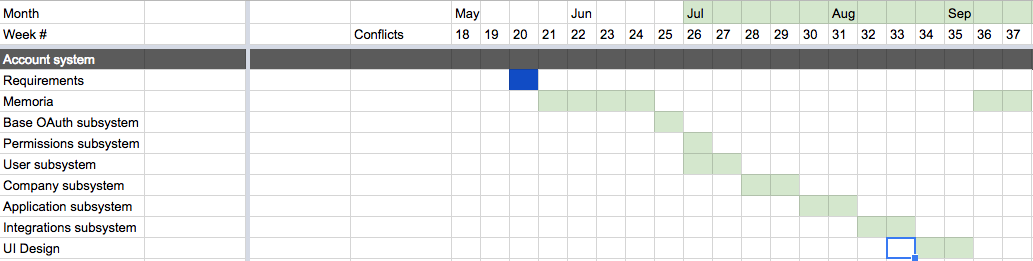
\includegraphics{source/figures/gantt.png}
\caption{Diagrama de Gantt \label{gantt}}
\end{figure}

\chapter{Descripción general del
proyecto}\label{descripciuxf3n-general-del-proyecto}

Este proyecto tiene la condición de Software Libre, por lo que en caso
de necesitar ser ampliado, cualquier persona podria hacerlo. El proyecto
es una aplicación nueva, no es continuación de otro proyecto

\section{Descripción}\label{descripciuxf3n}

El proyecto consiste en una aplicación web, con una API pública, con
distintos perfiles de usuario, en la que se llevará a cabo la
configuración de las aplicaciones que tienen acceso al sistema.

\section{Perfiles de usuario}\label{perfiles-de-usuario}

A continuación se expondrán los diferentes perfiles detallando a que
funcionalidad tendrá acceso cada uno.

\subsection{Perfil Administrador}\label{perfil-administrador}

El administrador tendrá acceso a toda la gestión de usuarios, de
productos y permisos. Por tanto el administrador podra crear nuevos
usuarios con los perfiles que considere necesarios, nuevas aplicaciones
y otorgar acceso a usuarios sobre aplicaciones.

\subsection{Perfil Gestor de
aplicaciones}\label{perfil-gestor-de-aplicaciones}

Este perfil solo tendrá acceso a gestionar las aplicaciones existentes
en el sistema, podrá también otorgar permisos sobre aplicaciones
existentes a usuarios.

\subsection{Perfil Usuario}\label{perfil-usuario}

Únicamente tendrá acceso a las aplicaciones visibles para este usuario.

\section{Interfaz de Usuario}\label{interfaz-de-usuario}

La interfaz será simple y funcional, ya que solo se utilizará a nivel
interno en cada empresa. Visualizada en un navegador web, con un menú
principal en el que se tendrá acceso a las diferentes funcionalidades,
estando ocultas las que no pertenezcan al perfil del usuario.

\section{Software}\label{software}

Al ser una aplicación web, ésta será multiplataforma, pudiendo funcionar
sobre cualquier navegador actual, ya que cumple los estándares de la
W3C.

Como lenguaje de servidor la aplicación utiliza Python, se toma la
decisión de utilizarlo por la amplia documentación que hay disponible,
por el conocimiento del desarrollador, además de la multitud de
librerías que existen para simplificar su utilización. Además se ha
utilizado el framework MVC Django, que simplifica muchas tareas que de
implementarlas únicamente con Python sin la ayuda de ninguna librería se
harían muy tediosas.

Para las vistas se ha utilizado HTML, CSS y JavaScript, además de
Bootstrap para simplificar el diseño de la aplicación, que es algo que
escapa al alcance de este proyecto.

En la parte de los datos se ha usado MySQL como SGBD, utilizando Django
ORM para abstraer el uso de la base de datos dentro de la aplicación.

\chapter{Análisis}\label{anuxe1lisis}

\section{Metodología de desarrollo}\label{metodologuxeda-de-desarrollo}

Para la realización del proyecto y su documentación se ha utilizado el
Rational Unified Process (RUP), junto con el Lenguaje Unificado de
Modelado (UML). Se ha elegido este sistema ya que es la metodología
estándar más utilizada, además de ser un grupo de metodologías que se
adaptan muy bien a las necesidades de un producto.

\section{Especificación de requisitos del
sistema}\label{especificaciuxf3n-de-requisitos-del-sistema}

A continuación se enumeran los requisitos funcionales que se consideran
fundamentales para el sistema. Éstos serán detallados utilizando casos
de uso, describiendo tanto su escenario principal como sus posibles
flujos alternativos. Además se detallará cada caso de uso con su
diagrama de secuencia correspondiente.

\subsection{Gestión de instalación}\label{gestiuxf3n-de-instalaciuxf3n}

Una vez finalizada la instalación de la aplicación el administrador de
la empresa debe terminar la configuración del sistema.

\begin{figure}
\centering
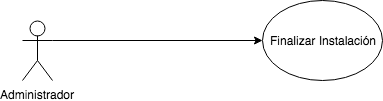
\includegraphics[width=0.50000\textwidth]{source/figures/gestion-instalacion.png}
\caption{Diagrama de casos de uso de Gestión de instalación
\label{gestion_instalacion}}
\end{figure}

\subsubsection{Caso de uso: Finalizar
instalación}\label{caso-de-uso-finalizar-instalaciuxf3n}

\begin{itemize}
\tightlist
\item
  \textbf{Descripción}: Caso de uso para la primera vez que se accede al
  sistema.
\item
  \textbf{Actores}: Administrador de la empresa.
\item
  \textbf{Precondiciones}: La aplicación ha sido instalada.
\item
  \textbf{Postcondiciones}: La aplicación queda configurada para su uso.
\item
  \textbf{Escenario principal}:

  \begin{itemize}
  \tightlist
  \item
    El sistema muestra un formulario al usuario para que introduzca los
    datos.
  \item
    El administrador introduce el nombre de la empresa, su email y su
    contraseña, que será la contraseña del administrador del sistema.
  \item
    El sistema valida los datos y muestra al usuario un formulario para
    introducir usuarios junto con su rol de acceso.
  \item
    El administrador repite el paso anterior hasta que termine de
    introducir usuarios
  \item
    El sistema manda un mail a todos los usuarios introducidos para
    terminar su configuración
  \item
    El sistema queda configurado.
  \end{itemize}
\item
  \textbf{Escenarios alternativos}:

  \begin{itemize}
  \tightlist
  \item
    Alguno de los datos introducidos es inválido.

    \begin{itemize}
    \tightlist
    \item
      El sistema indica el error y el caso de uso vuelve al paso
      anterior.
    \end{itemize}
  \item
    El administrador decide dejar el proceso de introducción de usuarios
    para más tarde.

    \begin{itemize}
    \tightlist
    \item
      El caso de uso termina.
    \end{itemize}
  \item
    El administrador introduce un email que ya ha introducido
    previamente.

    \begin{itemize}
    \tightlist
    \item
      El sistema indica el error y el caso de uso vuelve al paso
      anterior.
    \end{itemize}
  \end{itemize}
\end{itemize}

\subsection{Gestión de usuarios}\label{gestiuxf3n-de-usuarios}

\begin{figure}
\centering
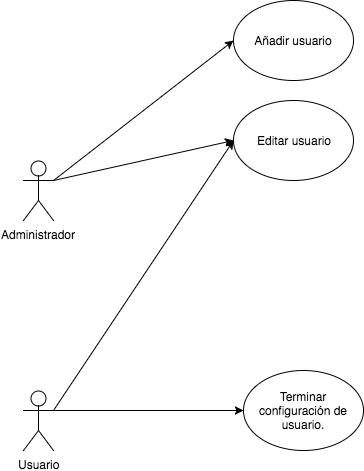
\includegraphics[width=0.50000\textwidth]{source/figures/gestion-usuarios.png}
\caption{Diagrama de casos de uso de Gestión de usuarios
\label{gestion_usuarios}}
\end{figure}

\subsubsection{Caso de uso: Añadir
usuario}\label{caso-de-uso-auxf1adir-usuario}

\begin{itemize}
\tightlist
\item
  \textbf{Descripción}: Caso de uso para la creación de un usuario.
\item
  \textbf{Actores}: Administrador de empresa.
\item
  \textbf{Precondiciones}: El administrador se ha identificado
  correctamente en el sistema.
\item
  \textbf{Postcondiciones}: Se crea un usuario con el perfil
  correspondiente.
\item
  \textbf{Escenario principal}:

  \begin{itemize}
  \tightlist
  \item
    El administrador selecciona una empresa existente para añadir un
    usuario en ella.
  \item
    El administrador introduce los datos del usuario y el nivel de
    privilegios.
  \item
    El sistema valida que los datos son correctos y no hay ningún
    usuario con el mismo email.
  \item
    El sistema crea el usuario y envía un mail al usuario para terminar
    la configuración
  \end{itemize}
\item
  \textbf{Escenarios alternativos}:

  \begin{itemize}
  \tightlist
  \item
    Alguno de los datos no es correcto.

    \begin{itemize}
    \tightlist
    \item
      El sistema indica el error y el caso de uso vuelve al paso
      anterior.
    \end{itemize}
  \item
    Ya existe algún usuario con el mismo email.

    \begin{itemize}
    \tightlist
    \item
      El sistema indica el error y el caso de uso vuelve al paso
      anterior.
    \end{itemize}
  \item
    En cualquier momento el administrador decide cancelar el proceso.

    \begin{itemize}
    \tightlist
    \item
      El caso de uso finaliza.
    \end{itemize}
  \end{itemize}
\end{itemize}

\subsubsection{Caso de uso: Terminar configuración de
usuario}\label{caso-de-uso-terminar-configuraciuxf3n-de-usuario}

\begin{itemize}
\tightlist
\item
  \textbf{Descripción}: El usuario registrado termina su configuración.
\item
  \textbf{Actores}: Usuario
\item
  \textbf{Precondiciones}: El usuario ha sido creado previamente por un
  administrador y el usuario ha recibido un email con un enlace.
\item
  \textbf{Postcondiciones}: El usuario queda configurado y con acceso al
  sistema.
\item
  \textbf{Escenario principal}:

  \begin{itemize}
  \tightlist
  \item
    El usuario abre el link que ha recibido por email.
  \item
    El sistema muestra un formulario para configurar la contraseña y el
    resto de datos necesarios.
  \item
    El usuario introduce los datos.
  \item
    El sistema valida los datos.
  \item
    El sistema guarda los datos y da acceso al usuario.
  \end{itemize}
\item
  \textbf{Escenarios alternativos}:

  \begin{itemize}
  \tightlist
  \item
    Alguno de los datos es incorrecto

    \begin{itemize}
    \tightlist
    \item
      El sistema lo indica y vuelve al paso anterior.
    \end{itemize}
  \end{itemize}
\end{itemize}

\subsubsection{Caso de uso: Editar
usuario}\label{caso-de-uso-editar-usuario}

\begin{itemize}
\tightlist
\item
  \textbf{Descripción}: Caso de uso para la edición de un usuario.
\item
  \textbf{Actores}: Usuario.
\item
  \textbf{Precondiciones}: El usuario que se intenta editar coincide con
  el identificado en el sistema o bien el usuario identificado es un
  administrador.
\item
  \textbf{Postcondiciones}: Se actualizan los datos del usuario.
\item
  \textbf{Escenario principal}:

  \begin{itemize}
  \tightlist
  \item
    El sistema muestra los datos actuales del usuario.
  \item
    El usuario modifica sus datos.
  \item
    El sistema valida que los datos introducidos son correctos y no hay
    ningún otro usuario con el mismo email.
  \item
    El usuario elige guardar los datos.
  \item
    El sistema modifica el usuario.
  \end{itemize}
\item
  \textbf{Escenarios alternativos}:

  \begin{itemize}
  \tightlist
  \item
    Alguno de los datos no es correcto.

    \begin{itemize}
    \tightlist
    \item
      El sistema indica el error y el caso de uso vuelve al paso
      anterior.
    \end{itemize}
  \item
    Ya existe algún usuario con el mismo email.

    \begin{itemize}
    \tightlist
    \item
      El sistema indica el error y el caso de uso vuelve al paso
      anterior.
    \end{itemize}
  \item
    En cualquier momento el administrador decide cancelar el proceso.

    \begin{itemize}
    \tightlist
    \item
      El caso de uso finaliza.
    \end{itemize}
  \end{itemize}
\end{itemize}

\subsubsection{Caso de uso: Ver
usuario.}\label{caso-de-uso-ver-usuario.}

\begin{itemize}
\tightlist
\item
  \textbf{Descripción}: Caso de uso para seleccionar una empresa.
\item
  \textbf{Actores}: Usuario del sistema.
\item
  \textbf{Precondiciones}: El usuario tiene privilegios de usuario del
  sistema.
\item
  \textbf{Postcondiciones}: Se muestran los datos del usuario.
\item
  \textbf{Escenario principal}:

  \begin{itemize}
  \tightlist
  \item
    El usuario elige un usuario para ver sus datos.
  \item
    El sistema muestra los datos del usuario.
  \item
    El sistema muestra las aplicaciones a las que tiene acceso
    actualmente.
  \end{itemize}
\end{itemize}

\subsubsection{Caso de uso: Borrar
usuario}\label{caso-de-uso-borrar-usuario}

\begin{itemize}
\tightlist
\item
  \textbf{Descripción}: Caso de uso para el borrado de un usuario
\item
  \textbf{Actores}: Administrador.
\item
  \textbf{Precondiciones}: El usuario identificado en el sistema tiene
  permisos para borrar usuarios o bien es administrador de la empresa
  del usuario a borrar.
\item
  \textbf{Postcondiciones}: El usuario queda borrado
\item
  \textbf{Escenario principal}:

  \begin{itemize}
  \tightlist
  \item
    El usuario selecciona un usuario para borrarlo.
  \item
    El sistema muestra los datos actuales del usuario.
  \item
    El usuario confirma que quiere borrar al usuario.
  \item
    El sistema confirma el borrado.
  \end{itemize}
\item
  \textbf{Escenarios alternativos}:

  \begin{itemize}
  \tightlist
  \item
    En cualquier momento el administrador decide cancelar el proceso.

    \begin{itemize}
    \tightlist
    \item
      El caso de uso finaliza.
    \end{itemize}
  \end{itemize}
\end{itemize}

\subsection{Gestión de empresas}\label{gestiuxf3n-de-empresas}

A continuación se especifican los casos de uso necesarios para llevar a
cabo la gestión de las empresas clientes del sistema.

\begin{figure}
\centering
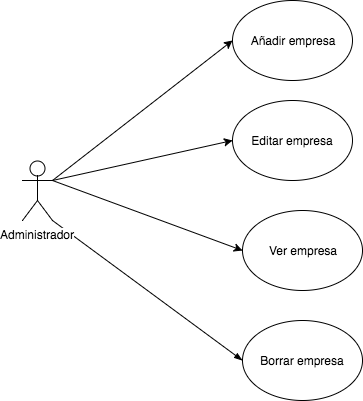
\includegraphics[width=0.50000\textwidth]{source/figures/gestion-empresas.png}
\caption{Diagrama de casos de uso de Gestión de empresas
\label{gestion_empresas}}
\end{figure}

\subsubsection{Caso de uso: Añadir
empresa}\label{caso-de-uso-auxf1adir-empresa}

\begin{itemize}
\tightlist
\item
  \textbf{Descripción}: Caso de uso para añadir una empresa
\item
  \textbf{Actores}: Administrador del sistema.
\item
  \textbf{Precondiciones}: El usuario tiene nivel de administrador del
  sistema.
\item
  \textbf{Postcondiciones}: La empresa queda registrada en el sistema
\item
  \textbf{Escenario principal}:

  \begin{itemize}
  \tightlist
  \item
    El administrador introduce los datos de la empresa.
  \item
    El sistema valida que los datos son correctos y no hay ninguna
    empresa con el mismo nombre.
  \item
    El administrador selecciona los productos a los que tendrá acceso la
    empresa.
  \item
    El sistema crea la empresa.
  \end{itemize}
\item
  \textbf{Escenarios alternativos}:

  \begin{itemize}
  \tightlist
  \item
    Alguno de los datos no es correcto.

    \begin{itemize}
    \tightlist
    \item
      El sistema indica el error y el caso de uso vuelve al paso
      anterior.
    \end{itemize}
  \item
    Ya existe alguna empresa con el mismo nombre.

    \begin{itemize}
    \tightlist
    \item
      El sistema indica el error y el caso de uso vuelve al paso
      anterior.
    \end{itemize}
  \item
    En cualquier momento el administrador decide cancelar el proceso.

    \begin{itemize}
    \tightlist
    \item
      El caso de uso finaliza.
    \end{itemize}
  \end{itemize}
\end{itemize}

\subsubsection{Caso de uso: Editar
empresa}\label{caso-de-uso-editar-empresa}

\begin{itemize}
\tightlist
\item
  \textbf{Descripción}: Caso de uso para la edición de una empresa.
\item
  \textbf{Actores}: Administrador del sistema.
\item
  \textbf{Precondiciones}: El usuario tiene privilegios de administrador
  del sistema.
\item
  \textbf{Postcondiciones}: Se actualizan los datos de la empresa
\item
  \textbf{Escenario principal}:

  \begin{itemize}
  \tightlist
  \item
    El sistema muestra los datos actuales de la empresa
  \item
    El usuario modifica sus datos.
  \item
    El sistema valida que los datos introducidos son correctos y no hay
    ningún otro usuario con el mismo email.
  \item
    El usuario modifica los productos a los que tiene acceso la empresa.
  \item
    El usuario elige guardar los datos.
  \item
    El sistema modifica la empresa.
  \end{itemize}
\item
  \textbf{Escenarios alternativos}:

  \begin{itemize}
  \tightlist
  \item
    Alguno de los datos no es correcto.

    \begin{itemize}
    \tightlist
    \item
      El sistema indica el error y el caso de uso vuelve al paso
      anterior.
    \end{itemize}
  \item
    En cualquier momento el administrador decide cancelar el proceso.

    \begin{itemize}
    \tightlist
    \item
      El caso de uso finaliza.
    \end{itemize}
  \end{itemize}
\end{itemize}

\subsubsection{Caso de uso: Ver
empresa.}\label{caso-de-uso-ver-empresa.}

\begin{itemize}
\tightlist
\item
  \textbf{Descripción}: Caso de uso para la edición de una empresa.
\item
  \textbf{Actores}: Usuario del sistema.
\item
  \textbf{Precondiciones}: El usuario tiene privilegios de usuario del
  sistema.
\item
  \textbf{Postcondiciones}: Se muestran los datos de la empresa
\item
  \textbf{Escenario principal}:

  \begin{itemize}
  \tightlist
  \item
    El usuario elige una empresa de las que tiene acceso.
  \item
    El sistema muestra los datos actuales de la empresa.
  \item
    El sistema muestra los usuarios de la empresa.
  \item
    El sistema muestra los productos contratados por la empresa.
  \end{itemize}
\end{itemize}

\subsubsection{Caso de uso: Borrar
empresa.}\label{caso-de-uso-borrar-empresa.}

\begin{itemize}
\tightlist
\item
  \textbf{Descripción}: Caso de uso para el borrado de una empresa.
\item
  \textbf{Actores}: Administrador.
\item
  \textbf{Precondiciones}: El usuario identificado en el sistema tiene
  permisos para borrar empresas.
\item
  \textbf{Postcondiciones}: La empresa queda borrada.
\item
  \textbf{Escenario principal}:

  \begin{itemize}
  \tightlist
  \item
    El usuario selecciona una empresa para borrarla.
  \item
    El sistema muestra los datos actuales de la empresa.
  \item
    El usuario confirma que quiere borrar a la empresa.
  \item
    El sistema confirma el borrado.
  \end{itemize}
\item
  \textbf{Escenarios alternativos}:

  \begin{itemize}
  \tightlist
  \item
    En cualquier momento el administrador decide cancelar el proceso.

    \begin{itemize}
    \tightlist
    \item
      El caso de uso finaliza.
    \end{itemize}
  \end{itemize}
\end{itemize}

\subsection{Gestión de productos}\label{gestiuxf3n-de-productos}

\begin{figure}
\centering
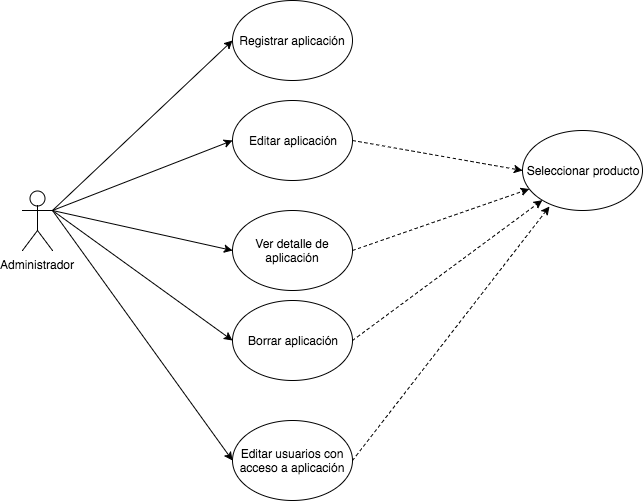
\includegraphics[width=0.50000\textwidth]{source/figures/gestion-productos.png}
\caption{Diagrama de casos de uso de Gestión de productos
\label{gestion_productos}}
\end{figure}

\subsubsection{Caso de uso: Seleccionar
producto}\label{caso-de-uso-seleccionar-producto}

\begin{itemize}
\tightlist
\item
  \textbf{Descripción}: Caso de uso abstracto incluído en otros casos de
  uso para seleccionar una aplicación de una lista de disponibles
\item
  \textbf{Actores}: Gestor de aplicaciones del sistema
\item
  \textbf{Precondiciones}: El usuario identificado en el sistema es un
  gestor de aplicaciones.
\item
  \textbf{Postcondiciones}: Se selecciona una aplicación para su uso en
  otra finalidad.
\item
  \textbf{Escenario principal}:

  \begin{itemize}
  \tightlist
  \item
    El sistema muestra un listado de las aplicaciones disponibles.
  \item
    El usuario selecciona la aplicación deseada.
  \end{itemize}
\item
  \textbf{Escenarios alternativos}:

  \begin{itemize}
  \tightlist
  \item
    No hay ninguna aplicación registrada.

    \begin{itemize}
    \tightlist
    \item
      El sistema indica el error y el caso de uso finaliza.
    \end{itemize}
  \end{itemize}
\end{itemize}

\subsubsection{Caso de uso: Registrar
aplicación}\label{caso-de-uso-registrar-aplicaciuxf3n}

\begin{itemize}
\tightlist
\item
  \textbf{Descripción}: Registra una nueva aplicación en el sistema.
\item
  \textbf{Actores}: Gestor de aplicaciones del sistema
\item
  \textbf{Precondiciones}: El usuario identificado en el sistema es un
  gestor de aplicaciones.
\item
  \textbf{Postcondiciones}: La aplicación queda registrada.
\item
  \textbf{Escenario principal}:

  \begin{itemize}
  \tightlist
  \item
    El gestor introduce el código, el nombre y todos los demás datos de
    la aplicación.
  \item
    El sistema comprueba que los datos cumplen el formato.
  \item
    El sistema confirma el alta de la aplicación mostrando un mensaje.
  \end{itemize}
\item
  \textbf{Escenarios alternativos}:

  \begin{itemize}
  \tightlist
  \item
    Alguno de los datos introducidos tiene un formato incorrecto.

    \begin{itemize}
    \tightlist
    \item
      El sistema indica el error y se vuelve al paso anterior.
    \end{itemize}
  \item
    Falta algún campo obligatorio.

    \begin{itemize}
    \tightlist
    \item
      El sistema indica el error y se vuelve al paso anterior.
    \end{itemize}
  \item
    Ya existe alguna aplicación con ese código o nombre,

    \begin{itemize}
    \tightlist
    \item
      El sistema indica el error y se vuelve al paso anterior.
    \end{itemize}
  \item
    El gestor decide cancelar el registro en cualquier momento

    \begin{itemize}
    \tightlist
    \item
      El caso de uso finaliza
    \end{itemize}
  \end{itemize}
\end{itemize}

\subsubsection{Caso de uso: Editar
aplicación}\label{caso-de-uso-editar-aplicaciuxf3n}

\begin{itemize}
\tightlist
\item
  \textbf{Descripción}: Edita una aplicación existente en el sistema
  modificando sus datos
\item
  \textbf{Actores}: Gestor de aplicaciones del sistema
\item
  \textbf{Precondiciones}: El usuario identificado en el sistema es un
  gestor de aplicaciones.
\item
  \textbf{Postcondiciones}: La aplicación queda modificada.
\item
  \textbf{Escenario principal}:

  \begin{itemize}
  \tightlist
  \item
    Se realiza el caso de uso \emph{seleccionar aplicación}
  \item
    El sistema muestra sus datos actuales, permitiendo su edición.
  \item
    El usuario modifica los datos.
  \item
    El sistema comprueba que los datos son correctos.
  \item
    El sistema confirma la modificación de la aplicación mostrando un
    mensaje.
  \end{itemize}
\item
  \textbf{Escenarios alternativos}:

  \begin{itemize}
  \tightlist
  \item
    Alguno de los datos introducidos tiene un formato incorrecto.

    \begin{itemize}
    \tightlist
    \item
      El sistema indica el error y se vuelve al paso anterior.
    \end{itemize}
  \item
    Falta algún campo obligatorio.

    \begin{itemize}
    \tightlist
    \item
      El sistema indica el error y se vuelve al paso anterior.
    \end{itemize}
  \item
    Ya existe alguna aplicación con ese código o nombre,

    \begin{itemize}
    \tightlist
    \item
      El sistema indica el error y se vuelve al paso anterior.
    \end{itemize}
  \item
    El gestor decide cancelar el registro en cualquier momento

    \begin{itemize}
    \tightlist
    \item
      El caso de uso finaliza
    \end{itemize}
  \end{itemize}
\end{itemize}

\subsubsection{Caso de uso: Borrar
aplicación}\label{caso-de-uso-borrar-aplicaciuxf3n}

\begin{itemize}
\tightlist
\item
  \textbf{Descripción}: Borra una aplicación del sistema.
\item
  \textbf{Actores}: Gestor de aplicaciones del sistema
\item
  \textbf{Precondiciones}: El usuario identificado en el sistema es un
  gestor de aplicaciones.
\item
  \textbf{Postcondiciones}: La aplicación queda eliminada.
\item
  \textbf{Escenario principal}:

  \begin{itemize}
  \tightlist
  \item
    Se realiza el caso de uso \emph{seleccionar aplicación}
  \item
    El sistema muestra un diálogo de confirmación.
  \item
    El usuario confirma que quiere eliminar la aplicación.
  \item
    El sistema elimina la aplicación.
  \item
    El sistema confirma la eliminación de la aplicación mostrando un
    mensaje.
  \end{itemize}
\item
  \textbf{Escenarios alternativos}:

  \begin{itemize}
  \tightlist
  \item
    El usuario selecciona que no desea eliminar la aplicación

    \begin{itemize}
    \tightlist
    \item
      El caso de uso se reinicia.
    \end{itemize}
  \item
    El gestor decide cancelar la eliminación en cualquier momento

    \begin{itemize}
    \tightlist
    \item
      El caso de uso finaliza
    \end{itemize}
  \end{itemize}
\end{itemize}

\subsubsection{Caso de uso: Ver detalle de
aplicación}\label{caso-de-uso-ver-detalle-de-aplicaciuxf3n}

\begin{itemize}
\tightlist
\item
  \textbf{Descripción}: Muestra los datos de una aplicación en detalle,
  así como sus credenciales.
\item
  \textbf{Actores}: Gestor de aplicaciones del sistema
\item
  \textbf{Precondiciones}: El usuario identificado en el sistema es un
  gestor de aplicaciones.
\item
  \textbf{Postcondiciones}: Los datos de la aplicación se muestran por
  pantqalla
\item
  \textbf{Escenario principal}:

  \begin{itemize}
  \tightlist
  \item
    Se realiza el caso de uso \emph{seleccionar aplicación}
  \item
    El sistema muestra los datos de la aplicación y sus credenciales.
  \end{itemize}
\item
  \textbf{Escenarios alternativos}:

  \begin{itemize}
  \tightlist
  \item
    El gestor decide cancelar el proceso en cualquier momento

    \begin{itemize}
    \tightlist
    \item
      El caso de uso finaliza
    \end{itemize}
  \end{itemize}
\end{itemize}

\subsubsection{Caso de uso: Editar usuarios de la empresa con acceso a
la
aplicación}\label{caso-de-uso-editar-usuarios-de-la-empresa-con-acceso-a-la-aplicaciuxf3n}

\begin{itemize}
\tightlist
\item
  \textbf{Descripción}: Cambia los usuarios de una empresa que tienen
  acceso a la aplicación.
\item
  \textbf{Actores}: Administrador de empresa.
\item
  \textbf{Precondiciones}: El usuario identificado en el sistema es un
  administrador de una empresa.
\item
  \textbf{Postcondiciones}: Los usuarios con acceso a la aplicación
  quedan modificados.
\item
  \textbf{Escenario principal}:

  \begin{itemize}
  \tightlist
  \item
    Se realiza el caso de uso \emph{seleccionar aplicación}
  \item
    El usuario selecciona el rol que quiere editar.
  \item
    El usuario selecciona los usuarios de su empresa a añadir a la
    aplicación.
  \item
    El usuario vuelve al paso 2 para seleccionar otro rol hasta que haya
    acabado con todos los roles.
  \item
    El usuario selecciona guardar.
  \item
    El sistema modifica los datos
  \end{itemize}
\item
  \textbf{Escenarios alternativos}:

  \begin{itemize}
  \tightlist
  \item
    El gestor decide cancelar el proceso en cualquier momento

    \begin{itemize}
    \tightlist
    \item
      El caso de uso finaliza
    \end{itemize}
  \end{itemize}
\end{itemize}

\section{Gestión de incidencias}\label{gestiuxf3n-de-incidencias}

\subsubsection{Caso de uso: Crear incidencia de
aplicación}\label{caso-de-uso-crear-incidencia-de-aplicaciuxf3n}

\begin{itemize}
\tightlist
\item
  \textbf{Descripción}: Un usuario crea una incidencia relacionada con
  una aplicación.
\item
  \textbf{Actores}: Usuario
\item
  \textbf{Precondiciones}: El usuario tiene acceso a la aplicación
  seleccionada.
\item
  \textbf{Postcondiciones}: La incidencia queda registrada y visible
  para los administradores.
\item
  \textbf{Escenario principal}:

  \begin{itemize}
  \tightlist
  \item
    El usuario selecciona crear incidencia en una aplicación
  \item
    El sistema muestra el formulario de envío
  \item
    El usuario redacta la incidencia y la envía
  \item
    El sistema la registra como pendiente y queda visible a los
    administradores.
  \end{itemize}
\item
  \textbf{Escenarios alternativos}:

  \begin{itemize}
  \tightlist
  \item
    Las credenciales son incorrectas.

    \begin{itemize}
    \tightlist
    \item
      El sistema lo indica y vuelve al paso anterior.
    \end{itemize}
  \item
    La aplicación seleccionada no es accesible por el usuario

    \begin{itemize}
    \tightlist
    \item
      El sistema lo indica y el caso de uso termina
    \end{itemize}
  \item
    El usuario decide cancelar el proceso en cualquier momento

    \begin{itemize}
    \tightlist
    \item
      El caso de uso finaliza
    \end{itemize}
  \end{itemize}
\end{itemize}

\subsubsection{Caso de uso: Añadir comentario a
incidencia}\label{caso-de-uso-auxf1adir-comentario-a-incidencia}

\begin{itemize}
\tightlist
\item
  \textbf{Descripción}: Un usuario comenta una incidencia.
\item
  \textbf{Actores}: Usuario
\item
  \textbf{Precondiciones}: El usuario tiene acceso a la aplicación
  seleccionada y la incidencia ha sido registrada por un usuario de la
  empresa.
\item
  \textbf{Postcondiciones}: El comentario se añade
\item
  \textbf{Escenario principal}:

  \begin{itemize}
  \tightlist
  \item
    El usuario selecciona una incidencia creada por él y selecciona
    añadir un comentario.
  \item
    El sistema muestra el formulario.
  \item
    El usuario introduce los datos.
  \item
    El sistema lo guarda.
  \end{itemize}
\item
  \textbf{Escenarios alternativos}:

  \begin{itemize}
  \tightlist
  \item
    Las credenciales son incorrectas.

    \begin{itemize}
    \tightlist
    \item
      El sistema lo indica y vuelve al paso anterior.
    \end{itemize}
  \item
    La aplicación seleccionada no es accesible por el usuario

    \begin{itemize}
    \tightlist
    \item
      El sistema lo indica y el caso de uso termina
    \end{itemize}
  \item
    La incidencia seleccionada no ha sido creada por un usuario de la
    empresa.

    \begin{itemize}
    \tightlist
    \item
      El sistema lo indica y el caso de uso termina
    \end{itemize}
  \item
    El usuario decide cancelar el proceso en cualquier momento

    \begin{itemize}
    \tightlist
    \item
      El caso de uso finaliza
    \end{itemize}
  \end{itemize}
\end{itemize}

\subsubsection{Caso de uso: Cerrar
incidencia}\label{caso-de-uso-cerrar-incidencia}

\begin{itemize}
\tightlist
\item
  \textbf{Descripción}: Un usuario administrador completa una incidencia
\item
  \textbf{Actores}: Administrador
\item
  \textbf{Precondiciones}: El usuario es administrador
\item
  \textbf{Postcondiciones}: La incidencia queda resuelta
\item
  \textbf{Escenario principal}:

  \begin{itemize}
  \tightlist
  \item
    El usuario selecciona una incidencia.
  \item
    El sistema muestra los datos.
  \item
    El usuario selecciona completarla.
  \item
    El sistema muestra el formulario de resolución.
  \item
    El usuario redacta la resolución y envía.
  \item
    El sistema cierra la incidencia y notifica al creador.
  \end{itemize}
\item
  \textbf{Escenarios alternativos}:

  \begin{itemize}
  \tightlist
  \item
    Las credenciales son incorrectas.

    \begin{itemize}
    \tightlist
    \item
      El sistema lo indica y vuelve al paso anterior.
    \end{itemize}
  \item
    El usuario decide cancelar el proceso en cualquier momento

    \begin{itemize}
    \tightlist
    \item
      El caso de uso finaliza
    \end{itemize}
  \end{itemize}
\end{itemize}

\subsubsection{Caso de uso: Borrar
incidencia}\label{caso-de-uso-borrar-incidencia}

\begin{itemize}
\tightlist
\item
  \textbf{Descripción}: Un usuario borra una incidencia creada por él.
\item
  \textbf{Actores}: Usuario
\item
  \textbf{Precondiciones}: El usuario tiene acceso a la aplicación
  seleccionada.
\item
  \textbf{Postcondiciones}: La incidencia queda borrada.
\item
  \textbf{Escenario principal}:

  \begin{itemize}
  \tightlist
  \item
    El usuario selecciona una incidencia creada por él y selecciona
    borrarla.
  \item
    El sistema pide confirmación.
  \item
    El usuario confirma.
  \end{itemize}
\item
  \textbf{Escenarios alternativos}:

  \begin{itemize}
  \tightlist
  \item
    Las credenciales son incorrectas.

    \begin{itemize}
    \tightlist
    \item
      El sistema lo indica y vuelve al paso anterior.
    \end{itemize}
  \item
    La aplicación seleccionada no es accesible por el usuario

    \begin{itemize}
    \tightlist
    \item
      El sistema lo indica y el caso de uso termina
    \end{itemize}
  \item
    La incidencia seleccionada no ha sido creada por el usuario.

    \begin{itemize}
    \tightlist
    \item
      El sistema lo indica y el caso de uso termina
    \end{itemize}
  \item
    El usuario decide cancelar el proceso en cualquier momento

    \begin{itemize}
    \tightlist
    \item
      El caso de uso finaliza
    \end{itemize}
  \end{itemize}
\end{itemize}

\section{Gestión de mensajes}\label{gestiuxf3n-de-mensajes}

\subsubsection{Caso de uso: Enviar mensaje a otro
usuario}\label{caso-de-uso-enviar-mensaje-a-otro-usuario}

\begin{itemize}
\tightlist
\item
  \textbf{Descripción}: Un usuario envía un mensaje a otro
\item
  \textbf{Actores}: Usuario
\item
  \textbf{Precondiciones}: El destinatario está en la misma empresa que
  el usuario.
\item
  \textbf{Postcondiciones}: El destinatario recibe el mensaje enviado en
  su bandeja de entrada.
\item
  \textbf{Escenario principal}:

  \begin{itemize}
  \tightlist
  \item
    El usuario selecciona enviar un mensaje nuevo.
  \item
    El sistema muestra el formulario de envío
  \item
    El usuario selecciona el usuario destino
  \item
    El sistema marca el usuario seleccionado como destinatario
  \item
    El usuario redacta el mensaje y lo envía.
  \item
    El sistema envía el mensaje al destinatario
  \end{itemize}
\item
  \textbf{Escenarios alternativos}:

  \begin{itemize}
  \tightlist
  \item
    Las credenciales son incorrectas.

    \begin{itemize}
    \tightlist
    \item
      El sistema lo indica y vuelve al paso anterior.
    \end{itemize}
  \item
    El usuario destinatario no pertenece a la misma empresa

    \begin{itemize}
    \tightlist
    \item
      El sistema lo indica y el caso de uso termina
    \end{itemize}
  \item
    El usuario decide cancelar el proceso en cualquier momento

    \begin{itemize}
    \tightlist
    \item
      El caso de uso finaliza
    \end{itemize}
  \end{itemize}
\end{itemize}

\subsubsection{Caso de uso: Ver bandeja de
entrada}\label{caso-de-uso-ver-bandeja-de-entrada}

\begin{itemize}
\tightlist
\item
  \textbf{Descripción}: Se muestra la bandeja de entrada de un usuario.
\item
  \textbf{Actores}: Usuario
\item
  \textbf{Precondiciones}: El usuario existe y está logueado
\item
  \textbf{Postcondiciones}: Se muestra la bandeja de entrada con todos
  los mensajes recibidos.
\item
  \textbf{Escenario principal}:

  \begin{itemize}
  \tightlist
  \item
    El usuario selecciona Ver bandeja de entrada.
  \item
    El sistema muestra la lista de mensajes.
  \end{itemize}
\item
  \textbf{Escenarios alternativos}:

  \begin{itemize}
  \tightlist
  \item
    Las credenciales son incorrectas.

    \begin{itemize}
    \tightlist
    \item
      El sistema lo indica y vuelve al paso anterior.
    \end{itemize}
  \item
    El usuario decide cancelar el proceso en cualquier momento

    \begin{itemize}
    \tightlist
    \item
      El caso de uso finaliza
    \end{itemize}
  \end{itemize}
\end{itemize}

\subsubsection{Caso de uso: Ver mensaje}\label{caso-de-uso-ver-mensaje}

\begin{itemize}
\tightlist
\item
  \textbf{Descripción}: Se muestra la bandeja de entrada de un usuario.
\item
  \textbf{Actores}: Usuario
\item
  \textbf{Precondiciones}: El usuario existe y está logueado
\item
  \textbf{Postcondiciones}: Se muestra la bandeja de entrada con todos
  los mensajes recibidos.
\item
  \textbf{Escenario principal}:

  \begin{itemize}
  \tightlist
  \item
    El usuario selecciona un mensaje de su bandeja de entrada.
  \item
    El sistema muestra el contenido del mensaje.
  \end{itemize}
\item
  \textbf{Escenarios alternativos}:

  \begin{itemize}
  \tightlist
  \item
    Las credenciales son incorrectas.

    \begin{itemize}
    \tightlist
    \item
      El sistema lo indica y vuelve al paso anterior.
    \end{itemize}
  \item
    El usuario decide cancelar el proceso en cualquier momento

    \begin{itemize}
    \tightlist
    \item
      El caso de uso finaliza
    \end{itemize}
  \end{itemize}
\end{itemize}

\subsubsection{Caso de uso: Borrar
mensaje}\label{caso-de-uso-borrar-mensaje}

\begin{itemize}
\tightlist
\item
  \textbf{Descripción}: Se muestra la bandeja de entrada de un usuario.
\item
  \textbf{Actores}: Usuario
\item
  \textbf{Precondiciones}: El usuario existe y está logueado
\item
  \textbf{Postcondiciones}: Se muestra la bandeja de entrada con todos
  los mensajes recibidos.
\item
  \textbf{Escenario principal}:

  \begin{itemize}
  \tightlist
  \item
    El usuario selecciona un mensaje de su bandeja de entrada.
  \item
    El sistema muestra el contenido del mensaje.
  \end{itemize}
\item
  \textbf{Escenarios alternativos}:

  \begin{itemize}
  \tightlist
  \item
    Las credenciales son incorrectas.

    \begin{itemize}
    \tightlist
    \item
      El sistema lo indica y vuelve al paso anterior.
    \end{itemize}
  \item
    El usuario decide cancelar el proceso en cualquier momento

    \begin{itemize}
    \tightlist
    \item
      El caso de uso finaliza
    \end{itemize}
  \end{itemize}
\end{itemize}

\section{Gestión de Reglas de
conexión}\label{gestiuxf3n-de-reglas-de-conexiuxf3n}

\subsubsection{Caso de uso: Crear regla de acceso de
usuario}\label{caso-de-uso-crear-regla-de-acceso-de-usuario}

\begin{itemize}
\tightlist
\item
  \textbf{Descripción}: Se añade una regla para controlar las conexiones
  del usuario
\item
  \textbf{Actores}: Administrador de empresa
\item
  \textbf{Precondiciones}: El usuario existe en el sistema
\item
  \textbf{Postcondiciones}: La regla queda creada y se aplica en cada
  acceso del usuario
\item
  \textbf{Escenario principal}:

  \begin{itemize}
  \tightlist
  \item
    El administrador entra en el menú de crear reglas de usuario
  \item
    El sistema muestra el formulario para crear reglas
  \item
    El administrador añade nombre, selecciona operador y añade los
    parámetros
  \item
    El sistema valida los datos
  \item
    La regla queda aplicada.
  \end{itemize}
\item
  \textbf{Escenarios alternativos}:

  \begin{itemize}
  \tightlist
  \item
    Las credenciales son incorrectas.

    \begin{itemize}
    \tightlist
    \item
      El sistema lo indica y vuelve al paso anterior.
    \end{itemize}
  \item
    El usuario identificado no tiene acceso al usuario

    \begin{itemize}
    \tightlist
    \item
      El sistema lo indica y el caso de uso termina
    \end{itemize}
  \item
    Algún parámetro es incorrecto

    \begin{itemize}
    \tightlist
    \item
      El sistema lo indica y el caso de uso vuelve al paso anterior
    \end{itemize}
  \item
    El usuario decide cancelar el proceso en cualquier momento

    \begin{itemize}
    \tightlist
    \item
      El caso de uso finaliza
    \end{itemize}
  \end{itemize}
\end{itemize}

\subsubsection{Caso de uso: Crear regla de acceso de
empresa}\label{caso-de-uso-crear-regla-de-acceso-de-empresa}

\begin{itemize}
\tightlist
\item
  \textbf{Descripción}: Se añade una regla para controlar las conexiones
  de los usuarios de la empresa
\item
  \textbf{Actores}: Administrador de empresa
\item
  \textbf{Precondiciones}: El usuario existe en el sistema
\item
  \textbf{Postcondiciones}: La regla queda creada y se aplica en cada
  acceso de los usuarios de la empresa
\item
  \textbf{Escenario principal}:

  \begin{itemize}
  \tightlist
  \item
    El administrador entra en el menú de crear reglas de usuario
  \item
    El sistema muestra el formulario para crear reglas
  \item
    El administrador añade nombre, selecciona operador y añade los
    parámetros
  \item
    El sistema valida los datos
  \item
    La regla queda aplicada.
  \end{itemize}
\item
  \textbf{Escenarios alternativos}:

  \begin{itemize}
  \tightlist
  \item
    Las credenciales son incorrectas.

    \begin{itemize}
    \tightlist
    \item
      El sistema lo indica y vuelve al paso anterior.
    \end{itemize}
  \item
    El usuario identificado no tiene acceso al usuario

    \begin{itemize}
    \tightlist
    \item
      El sistema lo indica y el caso de uso termina
    \end{itemize}
  \item
    Algún parámetro es incorrecto

    \begin{itemize}
    \tightlist
    \item
      El sistema lo indica y el caso de uso vuelve al paso anterior
    \end{itemize}
  \item
    El usuario decide cancelar el proceso en cualquier momento

    \begin{itemize}
    \tightlist
    \item
      El caso de uso finaliza
    \end{itemize}
  \end{itemize}
\end{itemize}

\section{Gestión de configuración}\label{gestiuxf3n-de-configuraciuxf3n}

\subsubsection{Caso de uso: Añadir valor de configuración de
aplicación}\label{caso-de-uso-auxf1adir-valor-de-configuraciuxf3n-de-aplicaciuxf3n}

\begin{itemize}
\tightlist
\item
  \textbf{Descripción}: Se añade un valor de configuración para la
  aplicación. (Abstracto)
\item
  \textbf{Actores}: Administrador
\item
  \textbf{Precondiciones}: La aplicación existe en el sistema
\item
  \textbf{Postcondiciones}: El valor se añade a la configuración de
  aplicación
\item
  \textbf{Escenario principal}:

  \begin{itemize}
  \tightlist
  \item
    El administrador añade la clave de configuración
  \item
    El administrador añade el valor de configuración
  \item
    El sistema valida los datos
  \item
    El sistema los añade a la configuración
  \end{itemize}
\item
  \textbf{Escenarios alternativos}:

  \begin{itemize}
  \tightlist
  \item
    Las credenciales son incorrectas.

    \begin{itemize}
    \tightlist
    \item
      El sistema lo indica y vuelve al paso anterior.
    \end{itemize}
  \item
    Algún parámetro es incorrecto

    \begin{itemize}
    \tightlist
    \item
      El sistema lo indica y el caso de uso vuelve al paso anterior
    \end{itemize}
  \item
    El usuario decide cancelar el proceso en cualquier momento

    \begin{itemize}
    \tightlist
    \item
      El caso de uso finaliza
    \end{itemize}
  \end{itemize}
\end{itemize}

\subsubsection{Caso de uso: Borrar valor de configuración de
aplicación}\label{caso-de-uso-borrar-valor-de-configuraciuxf3n-de-aplicaciuxf3n}

\begin{itemize}
\tightlist
\item
  \textbf{Descripción}: Se borra un valor de configuración para la
  aplicación. (Abstracto)
\item
  \textbf{Actores}: Administrador
\item
  \textbf{Precondiciones}: El valor existe en la configuración de la
  aplicación
\item
  \textbf{Postcondiciones}: El valor se borra de la configuración de
  aplicación
\item
  \textbf{Escenario principal}:

  \begin{itemize}
  \tightlist
  \item
    El administrador selecciona la clave a borrar
  \item
    El sistema pide confirmación
  \item
    El administrador confirma el borrado
  \item
    El sistema elimina el valor
  \end{itemize}
\item
  \textbf{Escenarios alternativos}:

  \begin{itemize}
  \tightlist
  \item
    Las credenciales son incorrectas.

    \begin{itemize}
    \tightlist
    \item
      El sistema lo indica y vuelve al paso anterior.
    \end{itemize}
  \item
    El usuario decide cancelar el proceso en cualquier momento

    \begin{itemize}
    \tightlist
    \item
      El caso de uso finaliza
    \end{itemize}
  \item
    El usuario rechaza la confirmación

    \begin{itemize}
    \tightlist
    \item
      El caso de uso finaliza
    \end{itemize}
  \end{itemize}
\end{itemize}

\subsubsection{Caso de uso: Crear configuración de
aplicación}\label{caso-de-uso-crear-configuraciuxf3n-de-aplicaciuxf3n}

\begin{itemize}
\tightlist
\item
  \textbf{Descripción}: Se crea un set de metadatos de configuración
  para la aplicación
\item
  \textbf{Actores}: Administrador
\item
  \textbf{Precondiciones}: La aplicación existe en el sistema
\item
  \textbf{Postcondiciones}: El set de configuración se añade a la
  aplicación
\item
  \textbf{Escenario principal}:

  \begin{itemize}
  \tightlist
  \item
    El administrador entra en el menú de la aplicación y elige crear
    configuración
  \item
    El sistema muestra el formulario
  \item
    Se realiza el caso de uso \emph{añadir valor de configuración}
    tantas veces como sea necesario.
  \item
    La configuración se añade a la aplicación
  \end{itemize}
\item
  \textbf{Escenarios alternativos}:

  \begin{itemize}
  \tightlist
  \item
    Las credenciales son incorrectas.

    \begin{itemize}
    \tightlist
    \item
      El sistema lo indica y vuelve al paso anterior.
    \end{itemize}
  \item
    El usuario decide cancelar el proceso en cualquier momento

    \begin{itemize}
    \tightlist
    \item
      El caso de uso finaliza
    \end{itemize}
  \end{itemize}
\end{itemize}

\subsubsection{Caso de uso: Editar configuración de
aplicación}\label{caso-de-uso-editar-configuraciuxf3n-de-aplicaciuxf3n}

\begin{itemize}
\tightlist
\item
  \textbf{Descripción}: Editar un set de configuración ya creado
\item
  \textbf{Actores}: Administrador
\item
  \textbf{Precondiciones}: La aplicación existe en el sistema y tiene
  una configuración creada
\item
  \textbf{Postcondiciones}: El set de configuración queda modificado
\item
  \textbf{Escenario principal}:

  \begin{itemize}
  \tightlist
  \item
    El administrador entra en el menú de la aplicación y elige editar su
    configuración
  \item
    El sistema muestra el formulario con los valores precargados
  \item
    Se realiza el caso de uso \emph{añadir valor de configuración}
    tantas veces como sea necesario.
  \item
    Se realiza el caso de uso \emph{eliminar valor de configuración}
    tantas veces como sea necesario.
  \item
    La configuración queda modificada.
  \end{itemize}
\item
  \textbf{Escenarios alternativos}:

  \begin{itemize}
  \tightlist
  \item
    Las credenciales son incorrectas.

    \begin{itemize}
    \tightlist
    \item
      El sistema lo indica y vuelve al paso anterior.
    \end{itemize}
  \item
    El usuario decide cancelar el proceso en cualquier momento

    \begin{itemize}
    \tightlist
    \item
      El caso de uso finaliza
    \end{itemize}
  \end{itemize}
\end{itemize}

\subsubsection{Caso de uso: Borrar configuración de
aplicación}\label{caso-de-uso-borrar-configuraciuxf3n-de-aplicaciuxf3n}

\begin{itemize}
\tightlist
\item
  \textbf{Descripción}: Borrar un set de configuración ya creado
\item
  \textbf{Actores}: Administrador
\item
  \textbf{Precondiciones}: La aplicación existe en el sistema y tiene
  una configuración creada
\item
  \textbf{Postcondiciones}: El set de configuración queda borrado
\item
  \textbf{Escenario principal}:

  \begin{itemize}
  \tightlist
  \item
    El administrador entra en el menú de la aplicación y elige borrar su
    configuración
  \item
    El sistema pide confirmación
  \item
    El administrador confirma
  \item
    El set de configuración queda eliminado.
  \end{itemize}
\item
  \textbf{Escenarios alternativos}:

  \begin{itemize}
  \tightlist
  \item
    Las credenciales son incorrectas.

    \begin{itemize}
    \tightlist
    \item
      El sistema lo indica y vuelve al paso anterior.
    \end{itemize}
  \item
    El usuario decide cancelar el proceso en cualquier momento

    \begin{itemize}
    \tightlist
    \item
      El caso de uso finaliza
    \end{itemize}
  \item
    El usuario rechaza la confirmación

    \begin{itemize}
    \tightlist
    \item
      El caso de uso finaliza
    \end{itemize}
  \end{itemize}
\end{itemize}

\subsubsection{Caso de uso: Añadir valor de configuración de aplicación
para
empresa}\label{caso-de-uso-auxf1adir-valor-de-configuraciuxf3n-de-aplicaciuxf3n-para-empresa}

\begin{itemize}
\tightlist
\item
  \textbf{Descripción}: Se añade un valor de configuración de empresa
  para la aplicación. (Abstracto)
\item
  \textbf{Actores}: Administrador de empresa
\item
  \textbf{Precondiciones}: La aplicación existe en el sistema
\item
  \textbf{Postcondiciones}: El valor se añade a la configuración de
  aplicación de empresa
\item
  \textbf{Escenario principal}:

  \begin{itemize}
  \tightlist
  \item
    El administrador añade la clave de configuración
  \item
    El administrador añade el valor de configuración
  \item
    El sistema valida los datos
  \item
    El sistema los añade a la configuración
  \end{itemize}
\item
  \textbf{Escenarios alternativos}:

  \begin{itemize}
  \tightlist
  \item
    Las credenciales son incorrectas.

    \begin{itemize}
    \tightlist
    \item
      El sistema lo indica y vuelve al paso anterior.
    \end{itemize}
  \item
    Algún parámetro es incorrecto

    \begin{itemize}
    \tightlist
    \item
      El sistema lo indica y el caso de uso vuelve al paso anterior
    \end{itemize}
  \item
    El usuario decide cancelar el proceso en cualquier momento

    \begin{itemize}
    \tightlist
    \item
      El caso de uso finaliza
    \end{itemize}
  \end{itemize}
\end{itemize}

\subsubsection{Caso de uso: Borrar valor de configuración de aplicación
de
empresa}\label{caso-de-uso-borrar-valor-de-configuraciuxf3n-de-aplicaciuxf3n-de-empresa}

\begin{itemize}
\tightlist
\item
  \textbf{Descripción}: Se borra un valor de configuración para la
  aplicación. (Abstracto)
\item
  \textbf{Actores}: Administrador
\item
  \textbf{Precondiciones}: El valor existe en la configuración de la
  aplicación
\item
  \textbf{Postcondiciones}: El valor se borra de la configuración de
  aplicación
\item
  \textbf{Escenario principal}:

  \begin{itemize}
  \tightlist
  \item
    El administrador selecciona la clave a borrar
  \item
    El sistema pide confirmación
  \item
    El administrador confirma el borrado
  \item
    El sistema elimina el valor
  \end{itemize}
\item
  \textbf{Escenarios alternativos}:

  \begin{itemize}
  \tightlist
  \item
    Las credenciales son incorrectas.

    \begin{itemize}
    \tightlist
    \item
      El sistema lo indica y vuelve al paso anterior.
    \end{itemize}
  \item
    El usuario decide cancelar el proceso en cualquier momento

    \begin{itemize}
    \tightlist
    \item
      El caso de uso finaliza
    \end{itemize}
  \item
    El usuario rechaza la confirmación

    \begin{itemize}
    \tightlist
    \item
      El caso de uso finaliza
    \end{itemize}
  \end{itemize}
\end{itemize}

\subsubsection{Caso de uso: Crear configuración de aplicación de
empresa}\label{caso-de-uso-crear-configuraciuxf3n-de-aplicaciuxf3n-de-empresa}

\begin{itemize}
\tightlist
\item
  \textbf{Descripción}: Se crea un set de metadatos de configuración
  para la aplicación
\item
  \textbf{Actores}: Administrador de empresa
\item
  \textbf{Precondiciones}: La aplicación existe en el sistema y la
  empresa tiene acceso a ella
\item
  \textbf{Postcondiciones}: El set de configuración se añade a la
  aplicación
\item
  \textbf{Escenario principal}:

  \begin{itemize}
  \tightlist
  \item
    El administrador entra en el menú de la aplicación y elige crear
    configuración
  \item
    El sistema muestra el formulario
  \item
    Se realiza el caso de uso \emph{añadir valor de configuración}
    tantas veces como sea necesario.
  \item
    La configuración se añade a la aplicación
  \end{itemize}
\item
  \textbf{Escenarios alternativos}:

  \begin{itemize}
  \tightlist
  \item
    Las credenciales son incorrectas.

    \begin{itemize}
    \tightlist
    \item
      El sistema lo indica y vuelve al paso anterior.
    \end{itemize}
  \item
    El usuario decide cancelar el proceso en cualquier momento

    \begin{itemize}
    \tightlist
    \item
      El caso de uso finaliza
    \end{itemize}
  \item
    La empresa del usuario no tiene acceso a esta aplicación

    \begin{itemize}
    \tightlist
    \item
      El caso de uso finaliza
    \end{itemize}
  \end{itemize}
\end{itemize}

\subsubsection{Caso de uso: Editar configuración de aplicación de
empresa}\label{caso-de-uso-editar-configuraciuxf3n-de-aplicaciuxf3n-de-empresa}

\begin{itemize}
\tightlist
\item
  \textbf{Descripción}: Editar un set de configuración ya creado
\item
  \textbf{Actores}: Administrador
\item
  \textbf{Precondiciones}: La aplicación existe en el sistema y tiene
  una configuración creada y la empresa tiene acceso a ella
\item
  \textbf{Postcondiciones}: El set de configuración queda modificado
\item
  \textbf{Escenario principal}:

  \begin{itemize}
  \tightlist
  \item
    El administrador entra en el menú de la aplicación y elige editar su
    configuración
  \item
    El sistema muestra el formulario con los valores precargados
  \item
    Se realiza el caso de uso \emph{añadir valor de configuración}
    tantas veces como sea necesario.
  \item
    Se realiza el caso de uso \emph{eliminar valor de configuración}
    tantas veces como sea necesario.
  \item
    La configuración queda modificada.
  \end{itemize}
\item
  \textbf{Escenarios alternativos}:

  \begin{itemize}
  \tightlist
  \item
    Las credenciales son incorrectas.

    \begin{itemize}
    \tightlist
    \item
      El sistema lo indica y vuelve al paso anterior.
    \end{itemize}
  \item
    El usuario decide cancelar el proceso en cualquier momento

    \begin{itemize}
    \tightlist
    \item
      El caso de uso finaliza
    \end{itemize}
  \item
    La empresa del usuario no tiene acceso a esta aplicación

    \begin{itemize}
    \tightlist
    \item
      El caso de uso finaliza
    \end{itemize}
  \end{itemize}
\end{itemize}

\subsubsection{Caso de uso: Borrar configuración de
aplicación}\label{caso-de-uso-borrar-configuraciuxf3n-de-aplicaciuxf3n-1}

\begin{itemize}
\tightlist
\item
  \textbf{Descripción}: Borrar un set de configuración ya creado
\item
  \textbf{Actores}: Administrador
\item
  \textbf{Precondiciones}: La aplicación existe en el sistema y tiene
  una configuración creada y la empresa tiene acceso a la aplicación
\item
  \textbf{Postcondiciones}: El set de configuración queda borrado
\item
  \textbf{Escenario principal}:

  \begin{itemize}
  \tightlist
  \item
    El administrador entra en el menú de la aplicación y elige borrar su
    configuración
  \item
    El sistema pide confirmación
  \item
    El administrador confirma
  \item
    El set de configuración queda eliminado.
  \end{itemize}
\item
  \textbf{Escenarios alternativos}:

  \begin{itemize}
  \tightlist
  \item
    Las credenciales son incorrectas.

    \begin{itemize}
    \tightlist
    \item
      El sistema lo indica y vuelve al paso anterior.
    \end{itemize}
  \item
    El usuario decide cancelar el proceso en cualquier momento

    \begin{itemize}
    \tightlist
    \item
      El caso de uso finaliza
    \end{itemize}
  \item
    El usuario rechaza la confirmación

    \begin{itemize}
    \tightlist
    \item
      El caso de uso finaliza
    \end{itemize}
  \item
    La empresa del usuario no tiene acceso a esta aplicación

    \begin{itemize}
    \tightlist
    \item
      El caso de uso finaliza
    \end{itemize}
  \end{itemize}
\end{itemize}

\section{Integraciones}\label{integraciones}

\begin{figure}
\centering
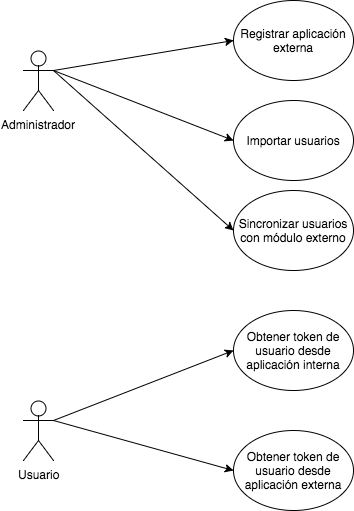
\includegraphics[width=0.50000\textwidth]{source/figures/gestion-integraciones.png}
\caption{Diagrama de casos de uso de integraciones
\label{gestion_integraciones}}
\end{figure}

\subsubsection{Caso de uso: Registrar aplicación
externa}\label{caso-de-uso-registrar-aplicaciuxf3n-externa}

\begin{itemize}
\tightlist
\item
  \textbf{Descripción}: Registra una nueva aplicación externa en el
  sistema.
\item
  \textbf{Actores}: Administrador de aplicaciones.
\item
  \textbf{Precondiciones}: El usuario identificado en el sistema es un
  administrador de aplicaciones.
\item
  \textbf{Postcondiciones}: La aplicación externa queda registrada.
\item
  \textbf{Escenario principal}:

  \begin{itemize}
  \tightlist
  \item
    El usuario introduce los datos de la aplicación.
  \item
    El sistema comprueba que son correctos.
  \item
    El usuario introduce la url externa para hacer la integración.
  \item
    El sistema prueba la conexión.
  \item
    El sistema guarda los datos.
  \end{itemize}
\item
  \textbf{Escenarios alternativos}:

  \begin{itemize}
  \tightlist
  \item
    Los datos son incorrectos.

    \begin{itemize}
    \tightlist
    \item
      El sistema lo indica y vuelve al paso anterior.
    \end{itemize}
  \item
    La conexión con la url externa no se puede realizar.

    \begin{itemize}
    \tightlist
    \item
      El sistema lo indica y vuelve al paso anterior.
    \end{itemize}
  \item
    El gestor decide cancelar el proceso en cualquier momento

    \begin{itemize}
    \tightlist
    \item
      El caso de uso finaliza
    \end{itemize}
  \end{itemize}
\end{itemize}

\subsubsection{Caso de uso: Obtener token de usuario desde aplicación
interna}\label{caso-de-uso-obtener-token-de-usuario-desde-aplicaciuxf3n-interna}

\begin{itemize}
\tightlist
\item
  \textbf{Descripción}: Un usuario obtiene un token a través de una
  aplicación interna.
\item
  \textbf{Actores}: Usuario
\item
  \textbf{Precondiciones}: El usuario existe en el sistema y tiene
  acceso a la aplicación.
\item
  \textbf{Postcondiciones}: La aplicación recibe el token de usuario.
\item
  \textbf{Escenario principal}:

  \begin{itemize}
  \tightlist
  \item
    La aplicación redirige al usuario a la web del sistema para
    identificarse.
  \item
    El usuario se identifica en el sistema.
  \item
    El sistema comprueba los datos son correctos.
  \item
    El sistema comprueba que el usuario tiene acceso a la aplicación.
  \item
    El sistema devuelve el token a la aplicación.
  \end{itemize}
\item
  \textbf{Escenarios alternativos}:

  \begin{itemize}
  \tightlist
  \item
    Las credenciales son incorrectas.

    \begin{itemize}
    \tightlist
    \item
      El sistema lo indica y vuelve al paso anterior.
    \end{itemize}
  \item
    El usuario identificado no tiene acceso a la aplicación.

    \begin{itemize}
    \tightlist
    \item
      El sistema lo indica y el caso de uso termina
    \end{itemize}
  \item
    El usuario decide cancelar el proceso en cualquier momento

    \begin{itemize}
    \tightlist
    \item
      El caso de uso finaliza
    \end{itemize}
  \end{itemize}
\end{itemize}

\subsubsection{Caso de uso: Obtener token de usuario desde apliación
externa}\label{caso-de-uso-obtener-token-de-usuario-desde-apliaciuxf3n-externa}

\begin{itemize}
\tightlist
\item
  \textbf{Descripción}: Un usuario obtiene un token a través de una
  aplicación externa.
\item
  \textbf{Actores}: Usuario
\item
  \textbf{Precondiciones}: El usuario existe en el sistema y tiene
  acceso a la aplicación.
\item
  \textbf{Postcondiciones}: La aplicación recibe el token de usuario.
\item
  \textbf{Escenario principal}:

  \begin{itemize}
  \tightlist
  \item
    La aplicación redirige al usuario a la web del sistema para
    identificarse.
  \item
    El usuario se identifica en la aplicación.
  \item
    El sistema redirige a la web de la aplicación externa.
  \item
    El usuario se identifica en la aplicación externa.
  \item
    El sistema devuelve el token a la aplicación.
  \end{itemize}
\item
  \textbf{Escenarios alternativos}:

  \begin{itemize}
  \tightlist
  \item
    Las credenciales son incorrectas.

    \begin{itemize}
    \tightlist
    \item
      El sistema lo indica y vuelve al paso anterior.
    \end{itemize}
  \item
    El usuario identificado no tiene acceso a la aplicación.

    \begin{itemize}
    \tightlist
    \item
      El sistema lo indica y el caso de uso termina
    \end{itemize}
  \item
    El usuario decide cancelar el proceso en cualquier momento

    \begin{itemize}
    \tightlist
    \item
      El caso de uso finaliza
    \end{itemize}
  \end{itemize}
\end{itemize}

\subsubsection{Caso de uso: Refrescar token de
usuario}\label{caso-de-uso-refrescar-token-de-usuario}

\begin{itemize}
\tightlist
\item
  \textbf{Descripción}: Un usuario obtiene un nuevo token a partir de un
  token de refresco
\item
  \textbf{Actores}: Usuario
\item
  \textbf{Precondiciones}: El usuario existe en el sistema y tiene
  acceso a la aplicación y tiene un token de refresco.
\item
  \textbf{Postcondiciones}: La aplicación recibe el token de usuario.
\item
  \textbf{Escenario principal}:

  \begin{itemize}
  \tightlist
  \item
    La aplicación intenta usar un token expirado.
  \item
    El sistema responde con un 401
  \item
    La aplicación manda una petición de refresco con el token de
    refresco.
  \item
    El sistema devuelve un nuevo token
  \end{itemize}
\item
  \textbf{Escenarios alternativos}:

  \begin{itemize}
  \tightlist
  \item
    Las credenciales son incorrectas.

    \begin{itemize}
    \tightlist
    \item
      El sistema lo indica y vuelve al paso anterior.
    \end{itemize}
  \item
    El usuario identificado no tiene acceso a la aplicación.

    \begin{itemize}
    \tightlist
    \item
      El sistema lo indica y el caso de uso termina
    \end{itemize}
  \item
    El usuario decide cancelar el proceso en cualquier momento

    \begin{itemize}
    \tightlist
    \item
      El caso de uso finaliza
    \end{itemize}
  \end{itemize}
\end{itemize}

\subsubsection{Caso de uso: Importar usuarios desde módulo
externo}\label{caso-de-uso-importar-usuarios-desde-muxf3dulo-externo}

\begin{itemize}
\tightlist
\item
  \textbf{Descripción}: Se importan usuarios desde módulo externo
\item
  \textbf{Actores}: Administrador de empresa
\item
  \textbf{Precondiciones}: El usuario existe en el sistema y es
  administrador de una empresa
\item
  \textbf{Postcondiciones}: Los usuarios quedan cargados en la
  aplicación
\item
  \textbf{Escenario principal}:

  \begin{itemize}
  \tightlist
  \item
    El usuario selecciona el método de importación.
  \item
    El usuario carga los datos siguiendo el método adecuado.
  \item
    El sistema registra los usuarios en el sistema.
  \end{itemize}
\end{itemize}

\subsubsection{Caso de uso: Sincronizar usuarios con módulo
externo}\label{caso-de-uso-sincronizar-usuarios-con-muxf3dulo-externo}

\begin{itemize}
\tightlist
\item
  \textbf{Descripción}: Se sincroniza con una api externa para cargar
  los usuarios.
\item
  \textbf{Actores}: Administrador de empresa
\item
  \textbf{Precondiciones}: El usuario existe en el sistema y es
  administrador de una empresa
\item
  \textbf{Postcondiciones}: Los usuarios quedan cargados en la
  aplicación
\item
  \textbf{Escenario principal}:

  \begin{itemize}
  \tightlist
  \item
    El usuario selecciona el método de importación.
  \item
    El usuario introduce las apis necesarias con las credenciales.
  \item
    El sistema sincroniza con la api externa.
  \end{itemize}
\end{itemize}

\section{Modelo Conceptual de datos}\label{modelo-conceptual-de-datos}

\begin{figure}
\centering
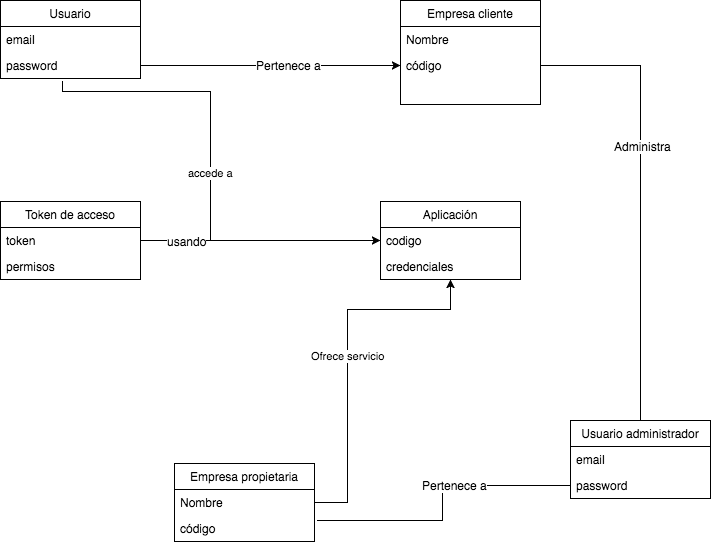
\includegraphics{source/figures/diagrama-clases-conceptual.png}
\caption{Diagrama de clases conceptual
\label{diagrama_clases_conceptual}}
\end{figure}

\section{Modelo de comportamiento del
sistema}\label{modelo-de-comportamiento-del-sistema}

Para el modelo de comportamiento del sistema se mostrarán diferentes
diagramas de secuencia del sistema. El diagrama define las interacciones
entre actores y sistema, también se detallarán los contratosde las
operaciones del sistema, para describir en detalle qué hace cada
operación.

Al existir muchos casos de uso similares, sólo se detallarán los más
relevantes de cada subsistema.

\subsection{Caso de uso: Añadir
usuario}\label{caso-de-uso-auxf1adir-usuario-1}

\begin{figure}
\centering
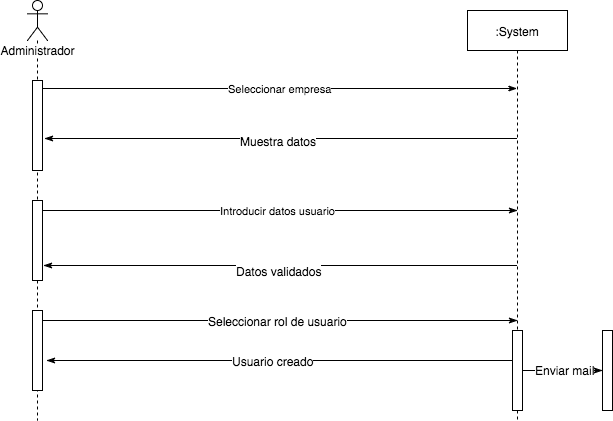
\includegraphics{source/figures/secuencia-anadir-usuario.png}
\caption{Caso de uso: Añadir usuario \label{secuencia_anadir_usuario}}
\end{figure}

\subsubsection{\texorpdfstring{Contrato de la operación ``introducir
datos de
usuario''}{Contrato de la operación introducir datos de usuario}}\label{contrato-de-la-operaciuxf3n-introducir-datos-de-usuario}

\begin{itemize}
\tightlist
\item
  \textbf{Responsabilidades}: Registrar usuario en el sistema
\item
  \textbf{Referencias cruzadas}: Caso de uso \emph{editar usuario}. Caso
  de uso \emph{añadir usuario}
\item
  \textbf{Precondiciones}: No existe un usuario con email = w\_email
\item
  \textbf{Postcondiciones}: Se crea una instancia de usuario U, se
  asignan w\_email y datos.
\end{itemize}

\subsection{Caso de uso: Editar
usuario}\label{caso-de-uso-editar-usuario-1}

\begin{figure}
\centering
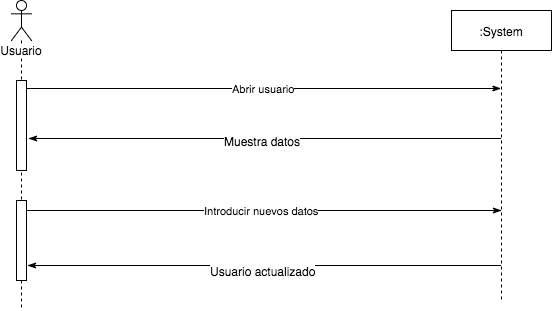
\includegraphics{source/figures/secuencia-editar-usuario.png}
\caption{Caso de uso: Editar usuario \label{secuencia_editar_usuario}}
\end{figure}

\subsubsection{\texorpdfstring{Contrato de la operación ``seleccionar
usuario''}{Contrato de la operación seleccionar usuario}}\label{contrato-de-la-operaciuxf3n-seleccionar-usuario}

\begin{itemize}
\tightlist
\item
  \textbf{Responsabilidades}: Abrir página de usuario
\item
  \textbf{Referencias cruzadas}: Caso de uso \emph{Ver usuario}. Caso de
  uso \emph{editar usuario}
\item
  \textbf{Precondiciones}: El usuario está creado en la empresa y el
  usuario logueado tiene permisos para verlo.
\item
  \textbf{Postcondiciones}: Se muestra la página del usuario.
\end{itemize}

\subsection{Caso de uso: Añadir
empresa}\label{caso-de-uso-auxf1adir-empresa-1}

\begin{figure}
\centering
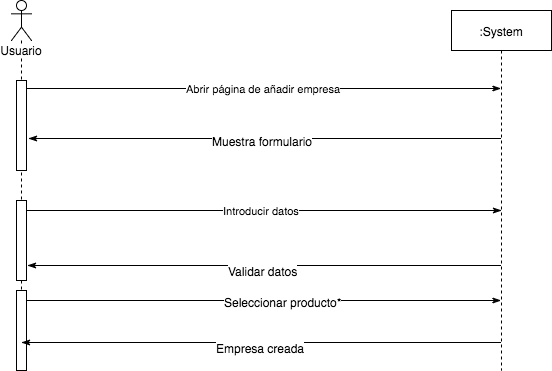
\includegraphics{source/figures/secuencia-anadir-empresa.png}
\caption{Caso de uso: Añadir empresa \label{secuencia_anadir_empresa}}
\end{figure}

\subsubsection{\texorpdfstring{Contrato de la operación ``introducir
datos de
empresa''}{Contrato de la operación introducir datos de empresa}}\label{contrato-de-la-operaciuxf3n-introducir-datos-de-empresa}

\begin{itemize}
\tightlist
\item
  \textbf{Responsabilidades}: Registrar empresa en el sistema
\item
  \textbf{Referencias cruzadas}: Caso de uso \emph{añadir empresa}. Caso
  de uso \emph{editar empresa}
\item
  \textbf{Precondiciones}: No existe una empresa con code = w\_code
\item
  \textbf{Postcondiciones}: Se crea una instancia de empresa E, se
  asignan w\_code y datos.
\end{itemize}

\subsection{Caso de uso: Editar
empresa}\label{caso-de-uso-editar-empresa-1}

\begin{figure}
\centering
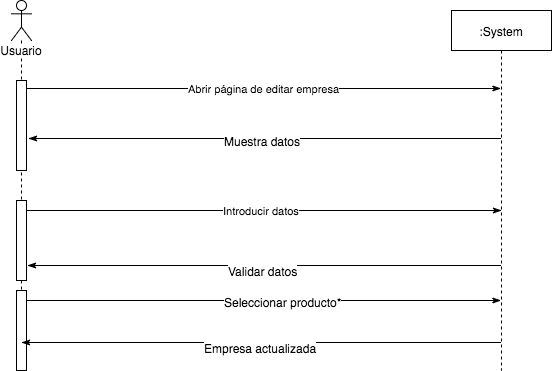
\includegraphics{source/figures/secuencia-editar-empresa.png}
\caption{Caso de uso: Editar empresa \label{secuencia_editar_empresa}}
\end{figure}

\subsubsection{\texorpdfstring{Contrato de la operación ``seleccionar
empresa''}{Contrato de la operación seleccionar empresa}}\label{contrato-de-la-operaciuxf3n-seleccionar-empresa}

\begin{itemize}
\tightlist
\item
  \textbf{Responsabilidades}: Abrir página de empresa
\item
  \textbf{Referencias cruzadas}: Caso de uso \emph{Ver empresa}. Caso de
  uso \emph{añadir usuario}. Caso de uso \emph{editar usuario}. Caso de
  uso \emph{editar empresa}. Caso de uso \emph{editar usuarios con
  acceso a aplicación}.
\item
  \textbf{Precondiciones}: La empresa existe en el sistema
\item
  \textbf{Postcondiciones}: Se muestra la página de la empresa con el
  listado de usuarios.
\end{itemize}

\subsection{Caso de uso: Añadir
aplicación}\label{caso-de-uso-auxf1adir-aplicaciuxf3n}

\begin{figure}
\centering
\includegraphics{source/figures/secuencia-anadir-aplicacion.png}
\caption{Caso de uso: Añadir aplicacion
\label{secuencia_anadir_aplicacion}}
\end{figure}

\subsubsection{\texorpdfstring{Contrato de la operación ``introducir
datos de
aplicación''}{Contrato de la operación introducir datos de aplicación}}\label{contrato-de-la-operaciuxf3n-introducir-datos-de-aplicaciuxf3n}

\begin{itemize}
\tightlist
\item
  \textbf{Responsabilidades}: Registrar aplicación en el sistema
\item
  \textbf{Referencias cruzadas}: Caso de uso \emph{añadir aplicación}.
  Caso de uso \emph{editar aplicación}
\item
  \textbf{Precondiciones}: No existe una aplicación con code = w\_code
\item
  \textbf{Postcondiciones}: Se crea una instancia de aplicación A, se
  asignan w\_code y datos, se generan credenciales.
\end{itemize}

\subsection{Caso de uso: Editar
aplicación}\label{caso-de-uso-editar-aplicaciuxf3n-1}

\begin{figure}
\centering
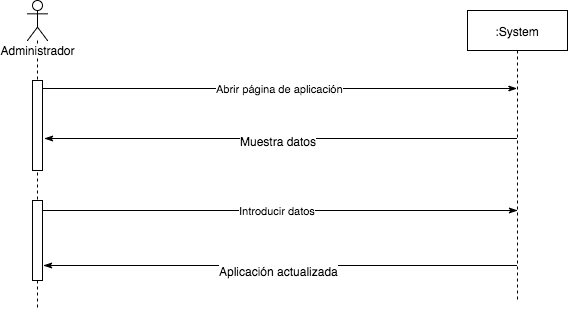
\includegraphics{source/figures/secuencia-editar-aplicacion.png}
\caption{Caso de uso: Editar aplicacion
\label{secuencia_editar_aplicacion}}
\end{figure}

\subsubsection{\texorpdfstring{Contrato de la operación ``seleccionar
aplicación''}{Contrato de la operación seleccionar aplicación}}\label{contrato-de-la-operaciuxf3n-seleccionar-aplicaciuxf3n}

\begin{itemize}
\tightlist
\item
  \textbf{Responsabilidades}: Abrir página de empresa
\item
  \textbf{Referencias cruzadas}: Caso de uso \emph{Ver aplicación}. Caso
  de uso \emph{editar aplicación}. Caso de uso \emph{borrar aplicación}
\item
  \textbf{Precondiciones}: La aplicación existe en el sistema
\item
  \textbf{Postcondiciones}: Se muestra la página de la aplicación.
\end{itemize}

\subsection{Caso de uso: Borrar
aplicación}\label{caso-de-uso-borrar-aplicaciuxf3n-1}

\begin{figure}
\centering
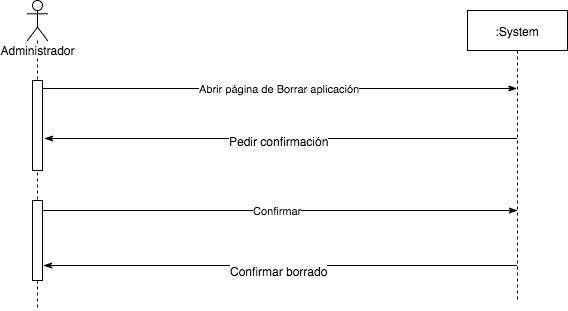
\includegraphics{source/figures/secuencia-borrar-aplicacion.png}
\caption{Caso de uso: Borrar aplicacion
\label{secuencia_borrar_aplicacion}}
\end{figure}

\subsubsection{\texorpdfstring{Contrato de la operación ``borrar
aplicación''}{Contrato de la operación borrar aplicación}}\label{contrato-de-la-operaciuxf3n-borrar-aplicaciuxf3n}

\begin{itemize}
\tightlist
\item
  \textbf{Responsabilidades}: Borra aplicación en el sistema
\item
  \textbf{Referencias cruzadas}: Caso de uso \emph{borrar aplicación}.
\item
  \textbf{Precondiciones}: Existe una aplicación con code = w\_code
\item
  \textbf{Postcondiciones}: Se elimina la instancia de aplicación A. Se
  borran todos los accesos existentes para la aplicación.
\end{itemize}

\subsection{Caso de uso: Editar usuarios de empresa con acceso a
aplicación}\label{caso-de-uso-editar-usuarios-de-empresa-con-acceso-a-aplicaciuxf3n}

\begin{figure}
\centering
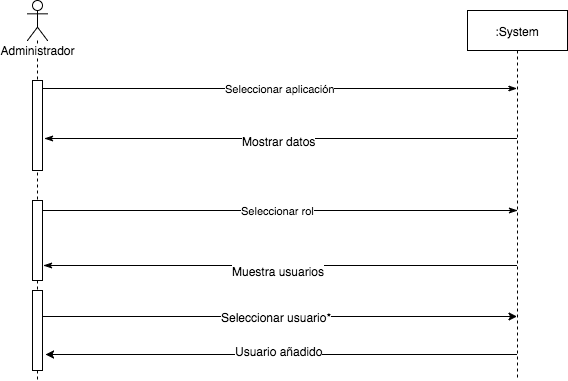
\includegraphics{source/figures/secuencia-editar-usuarios-empresa-aplicacion.png}
\caption{Caso de uso: Editar acceso de usuarios de empresa
\label{secuencia_editar_usuarios_empresa_aplicacion}}
\end{figure}

\subsection{Caso de uso: Obtener token de aplicación
interna}\label{caso-de-uso-obtener-token-de-aplicaciuxf3n-interna}

\begin{figure}
\centering
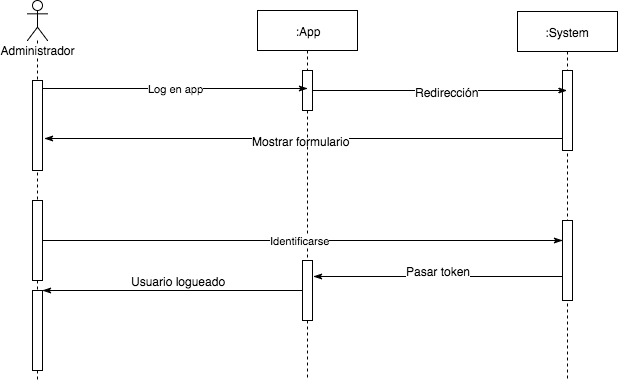
\includegraphics{source/figures/secuencia-obtener-token.png}
\caption{Caso de uso: Obtener token de aplicación interna
\label{secuencia_obtener_token}}
\end{figure}

\subsubsection{\texorpdfstring{Contrato de la operación ``obtener token
de
acceso''}{Contrato de la operación obtener token de acceso}}\label{contrato-de-la-operaciuxf3n-obtener-token-de-acceso}

\begin{itemize}
\tightlist
\item
  \textbf{Responsabilidades}: Genera un token para el usuario logueado.
\item
  \textbf{Referencias cruzadas}: Caso de uso \emph{Obtener token de
  aplicación interna}.
\item
  \textbf{Precondiciones}: El usuario tiene acceso a la aplicación.
\item
  \textbf{Postcondiciones}: Se genera un token de acceso para el
  usuario.
\end{itemize}

\chapter{Diseño}\label{diseuxf1o}

\section{Introducción}\label{introducciuxf3n-1}

La fase de diseño consiste en aplicar una serie de técnicas para
transformar los requisitos elicitados en la fase de análisis en una
estructura detallada para el sistema de forma que se pueda implementar
fácilmente a partir de ese diseño.

Este diseño ha de realizarse a varios niveles de detalle, por un lado a
nivel de arquitectura interna de la aplicación. Por otro lado el diseño
del modelo de datos y finalmente a más alto nivel detallar todos los
componentes del sistema y como interactúan entre si, componiendo un
sistema escalable.

Siguiendo los requisitos de la fase anterior, esta tarea es
relativamente sencilla y debe resultar en una serie de diagramas y
especificaciones que sirvan como guión y documentación a las personas
que vayan a participar, ahora o en un futuro en el desarrollo del
sistema.

Este documento debe contener también un modelo de despliegue incluyendo
infraestructura, aplicación y configuración.

\section{Arquitectura de
aplicación}\label{arquitectura-de-aplicaciuxf3n}

La aplicación se rige por el patrón arquitectónico MVC. Este patrón
permite separar la lógica de negocio de la presentación, así como de los
datos.

\begin{itemize}
\tightlist
\item
  El modelo representa a las estructuras de datos. Las clases del modelo
  contienen funciones para modificar los datos, insertar y actualizar la
  base de datos.
\item
  La vista es la información presentada al usuario. Una vista
  normalmente es una página web que puede contener datos del modelo para
  mostrarlos al usuario.
\item
  El controlador es un intermediario entre las dos capas anteriores y
  otros recursos que puedan ser necesarios. Se encarga de procesar las
  peticiones y generar la página web que será presentada al usuario.
\end{itemize}

Este patrón favorece la reutilización de código y la claridad.

\subsection{Elección del framework}\label{elecciuxf3n-del-framework}

Dado que en el lenguaje elegido para implementar la aplicación es
Python, se ha elegido el framework Django, debido a la experiencia
previa con esta tecnología. Este framework permite empezar a tener un
software funcionando en muy poco tiempo, dedicando el trabajo casi
exclusivamente a implementar el modelo y la lógica de negocio. Dado que
el framework ya es conocido, la curva de aprendizaje es mínima.

\subsection{Endpoints}\label{endpoints}

\subsubsection{Empresas}\label{empresas}

\paragraph{Visualización}\label{visualizaciuxf3n}

GET: /v1/companies

\begin{itemize}
\tightlist
\item
  Headers:

  \begin{itemize}
  \tightlist
  \item
    Content-Type: applicacion/json
  \item
    Authorization: Bearer \textless{}token\textgreater{}
  \end{itemize}
\item
  Response (Lista de):

  \begin{itemize}
  \tightlist
  \item
    \textbf{``id''}: 123,
  \item
    \textbf{``name''}: ``Company'',
  \item
    \textbf{``code''}: ``company\_1''
  \end{itemize}
\item
  Response codes:

  \begin{itemize}
  \tightlist
  \item
    200 OK (Success)
  \item
    401 UNAUTHORIZED (Token de acceso inválido o no enviado)
  \item
    403 FORBIDDEN (Sin permisos)
  \end{itemize}
\end{itemize}

GET: /v1/companies/\textless{}company-id\textgreater{}

\begin{itemize}
\tightlist
\item
  Headers:

  \begin{itemize}
  \tightlist
  \item
    Content-Type: application/json
  \item
    Authorization: Bearer \textless{}token\textgreater{}
  \end{itemize}
\item
  Response (JSON Object):

  \begin{itemize}
  \tightlist
  \item
    \textbf{``id''}: 123,
  \item
    \textbf{``name''}: ``Company'',
  \item
    \textbf{``code''}: ``company\_1''
  \end{itemize}
\item
  Response Codes:

  \begin{itemize}
  \tightlist
  \item
    200 OK (Success)
  \item
    401 UNAUTHORIZED (Token de acceso inválido o no enviado)
  \item
    403 FORBIDDEN (Sin permisos)
  \item
    404 NOT FOUND (\emph{company-id} no encontrado)
  \end{itemize}
\end{itemize}

\paragraph{Creación}\label{creaciuxf3n}

POST: /v1/companies

\begin{itemize}
\tightlist
\item
  Headers:

  \begin{itemize}
  \tightlist
  \item
    Content-Type: applicacion/json
  \item
    Authorization: Bearer \textless{}token\textgreater{}
  \end{itemize}
\item
  Request body (JSON Object):

  \begin{itemize}
  \tightlist
  \item
    \textbf{``name''}: ``Company'',
  \item
    \textbf{``code''}: ``company\_1''
  \end{itemize}
\item
  Response codes:

  \begin{itemize}
  \tightlist
  \item
    201 CREATED (Empresa creada)
  \item
    400 BAD REQUEST (Dato incorrecto en el body)
  \item
    401 UNAUTHORIZED (Token de acceso inválido o no enviado)
  \item
    403 FORBIDDEN (Sin permisos)
  \end{itemize}
\end{itemize}

\paragraph{Actualización}\label{actualizaciuxf3n}

PUT: /v1/companies/\textless{}company-id\textgreater{}

\begin{itemize}
\tightlist
\item
  Headers:

  \begin{itemize}
  \tightlist
  \item
    Content-Type: application/json
  \item
    Authorization: Bearer \textless{}token\textgreater{}
  \end{itemize}
\item
  Request body (JSON Object):

  \begin{itemize}
  \tightlist
  \item
    \textbf{``name''}: ``Company'',
  \item
    \textbf{``code''}: ``company\_id''
  \end{itemize}
\item
  Response codes:

  \begin{itemize}
  \tightlist
  \item
    200 OK (Empresa actualizada)
  \item
    400 BAD REQUEST (Dato incorrecto en el body)
  \item
    401 UNAUTHORIZED (Token de acceso inválido o no enviado)
  \item
    403 FORBIDDEN (Sin permisos)
  \end{itemize}
\end{itemize}

\paragraph{Borrado}\label{borrado}

DELETE: /v1/companies/\textless{}company-id\textgreater{}

\begin{itemize}
\tightlist
\item
  Headers:

  \begin{itemize}
  \tightlist
  \item
    Content-Type: application/json
  \item
    Authorization: Bearer \textless{}token\textgreater{}
  \end{itemize}
\item
  Response codes:

  \begin{itemize}
  \tightlist
  \item
    204 NO CONTENT (Empresa borrada)
  \item
    401 UNAUTHORIZED (Token de acceso inválido o no enviado)
  \item
    403 FORBIDDEN (Sin permisos)
  \end{itemize}
\end{itemize}

\subsubsection{Usuarios}\label{usuarios}

\paragraph{Visualización}\label{visualizaciuxf3n-1}

GET: /v1/companies/\textless{}company-id\textgreater{}/users

\begin{itemize}
\tightlist
\item
  Headers:

  \begin{itemize}
  \tightlist
  \item
    Content-Type: applicacion/json
  \item
    Authorization: Bearer \textless{}token\textgreater{}
  \end{itemize}
\item
  Response (Lista de):

  \begin{itemize}
  \tightlist
  \item
    \textbf{``id''}: 123,
  \item
    \textbf{``name''}: ``User'',
  \item
    \textbf{``email''}: ``user@company.com''
  \end{itemize}
\item
  Response codes:

  \begin{itemize}
  \tightlist
  \item
    200 OK (Success)
  \item
    401 UNAUTHORIZED (Token de acceso inválido o no enviado)
  \item
    403 FORBIDDEN (Sin permisos)
  \end{itemize}
\end{itemize}

GET:
/v1/companies/\textless{}company-id\textgreater{}/users/\textless{}user-id\textgreater{}

\begin{itemize}
\tightlist
\item
  Headers:

  \begin{itemize}
  \tightlist
  \item
    Content-Type: application/json
  \item
    Authorization: Bearer \textless{}token\textgreater{}
  \end{itemize}
\item
  Response (JSON Object):

  \begin{itemize}
  \tightlist
  \item
    \textbf{``id''}: 123,
  \item
    \textbf{``name''}: ``User'',
  \item
    \textbf{``email''}: ``email@company.com''
  \end{itemize}
\item
  Response Codes:

  \begin{itemize}
  \tightlist
  \item
    200 OK (Success)
  \item
    401 UNAUTHORIZED (Token de acceso inválido o no enviado)
  \item
    403 FORBIDDEN (Sin permisos)
  \item
    404 NOT FOUND (\emph{company-id} o \emph{user-id} no encontrado)
  \end{itemize}
\end{itemize}

\paragraph{Creación}\label{creaciuxf3n-1}

POST: /v1/companies/\textless{}company-id\textgreater{}/users

\begin{itemize}
\tightlist
\item
  Headers:

  \begin{itemize}
  \tightlist
  \item
    Content-Type: applicacion/json
  \item
    Authorization: Bearer \textless{}token\textgreater{}
  \end{itemize}
\item
  Request body (JSON Object):

  \begin{itemize}
  \tightlist
  \item
    \textbf{``name''}: ``Nombre'',
  \item
    \textbf{``email''}: ``user@company.com'',
  \item
    \textbf{``password''}: ``password''
  \end{itemize}
\item
  Response codes:

  \begin{itemize}
  \tightlist
  \item
    201 CREATED (Usuario creado)
  \item
    400 BAD REQUEST (Dato incorrecto en el body)
  \item
    401 UNAUTHORIZED (Token de acceso inválido o no enviado)
  \item
    403 FORBIDDEN (Sin permisos)
  \end{itemize}
\end{itemize}

\paragraph{Actualización}\label{actualizaciuxf3n-1}

PUT:
/v1/companies/\textless{}company-id\textgreater{}/users/\textless{}user-id\textgreater{}

\begin{itemize}
\tightlist
\item
  Headers:

  \begin{itemize}
  \tightlist
  \item
    Content-Type: application/json
  \item
    Authorization: Bearer \textless{}token\textgreater{}
  \end{itemize}
\item
  Request body (JSON Object):

  \begin{itemize}
  \tightlist
  \item
    \textbf{``name''}: ``User'',
  \item
    \textbf{``email''}: ``email@company.com''
  \item
    \textbf{``password''}: ``password''
  \end{itemize}
\item
  Response codes:

  \begin{itemize}
  \tightlist
  \item
    200 OK (Usuario actualizada)
  \item
    400 BAD REQUEST (Dato incorrecto en el body)
  \item
    401 UNAUTHORIZED (Token de acceso inválido o no enviado)
  \item
    403 FORBIDDEN (Sin permisos)
  \end{itemize}
\end{itemize}

\paragraph{Borrado}\label{borrado-1}

DELETE:
/v1/companies/\textless{}company-id\textgreater{}/users/\textless{}user-id\textgreater{}

\begin{itemize}
\tightlist
\item
  Headers:

  \begin{itemize}
  \tightlist
  \item
    Content-Type: application/json
  \item
    Authorization: Bearer \textless{}token\textgreater{}
  \end{itemize}
\item
  Response codes:

  \begin{itemize}
  \tightlist
  \item
    204 NO CONTENT (Usuario borrado)
  \item
    401 UNAUTHORIZED (Token de acceso inválido o no enviado)
  \item
    403 FORBIDDEN (Sin permisos)
  \end{itemize}
\end{itemize}

\subsubsection{Aplicaciones}\label{aplicaciones}

\paragraph{Visualización}\label{visualizaciuxf3n-2}

GET: /v1/applications

\begin{itemize}
\tightlist
\item
  Headers:

  \begin{itemize}
  \tightlist
  \item
    Content-Type: applicacion/json
  \item
    Authorization: Bearer \textless{}token\textgreater{}
  \end{itemize}
\item
  Response (Lista de):

  \begin{itemize}
  \tightlist
  \item
    \textbf{``id''}: 123,
  \item
    \textbf{``name''}: ``application'',
  \item
    \textbf{``client\_id''}: ``123123123'',
  \item
    \textbf{``client\_secret''}: ``123123123'',
  \end{itemize}
\item
  Response codes:

  \begin{itemize}
  \tightlist
  \item
    200 OK (Success)
  \item
    401 UNAUTHORIZED (Token de acceso inválido o no enviado)
  \item
    403 FORBIDDEN (Sin permisos)
  \end{itemize}
\end{itemize}

GET: /v1/applications/\textless{}client-id\textgreater{}

\begin{itemize}
\tightlist
\item
  Headers:

  \begin{itemize}
  \tightlist
  \item
    Content-Type: application/json
  \item
    Authorization: Bearer \textless{}token\textgreater{}
  \end{itemize}
\item
  Response (JSON Object):

  \begin{itemize}
  \tightlist
  \item
    \textbf{``id''}: 123,
  \item
    \textbf{``name''}: ``User'',
  \item
    \textbf{``client\_id''}: ``123123123'',
  \item
    \textbf{``client\_secret''}: ``123123123'',
  \end{itemize}
\item
  Response Codes:

  \begin{itemize}
  \tightlist
  \item
    200 OK (Success)
  \item
    401 UNAUTHORIZED (Token de acceso inválido o no enviado)
  \item
    403 FORBIDDEN (Sin permisos)
  \item
    404 NOT FOUND (\emph{client-id} no encontrado)
  \end{itemize}
\end{itemize}

\paragraph{Creación}\label{creaciuxf3n-2}

POST: /v1/applications/\textless{}client-id\textgreater{}

\begin{itemize}
\tightlist
\item
  Headers:

  \begin{itemize}
  \tightlist
  \item
    Content-Type: applicacion/json
  \item
    Authorization: Bearer \textless{}token\textgreater{}
  \end{itemize}
\item
  Request body (JSON Object):

  \begin{itemize}
  \tightlist
  \item
    \textbf{``name''}: ``Nombre'',
  \end{itemize}
\item
  Response (JSON Object):

  \begin{itemize}
  \tightlist
  \item
    \textbf{``id''}: 123,
  \item
    \textbf{``name''}: ``User'',
  \item
    \textbf{``client\_id''}: ``123123123'',
  \item
    \textbf{``client\_secret''}: ``123123123'',
  \end{itemize}
\item
  Response codes:

  \begin{itemize}
  \tightlist
  \item
    201 CREATED (Aplicación creada)
  \item
    400 BAD REQUEST (Dato incorrecto en el body)
  \item
    401 UNAUTHORIZED (Token de acceso inválido o no enviado)
  \item
    403 FORBIDDEN (Sin permisos)
  \end{itemize}
\end{itemize}

\paragraph{Actualización}\label{actualizaciuxf3n-2}

PUT: /v1/applications/\textless{}client-id\textgreater{}

\begin{itemize}
\tightlist
\item
  Headers:

  \begin{itemize}
  \tightlist
  \item
    Content-Type: application/json
  \item
    Authorization: Bearer \textless{}token\textgreater{}
  \end{itemize}
\item
  Request body (JSON Object):

  \begin{itemize}
  \tightlist
  \item
    \textbf{``name''}: ``User'',
  \end{itemize}
\item
  Response codes:

  \begin{itemize}
  \tightlist
  \item
    200 OK (Aplicación actualizada)
  \item
    400 BAD REQUEST (Dato incorrecto en el body)
  \item
    401 UNAUTHORIZED (Token de acceso inválido o no enviado)
  \item
    403 FORBIDDEN (Sin permisos)
  \end{itemize}
\end{itemize}

\paragraph{Borrado}\label{borrado-2}

DELETE: /v1/applications/\textless{}client-id\textgreater{}

\begin{itemize}
\tightlist
\item
  Headers:

  \begin{itemize}
  \tightlist
  \item
    Content-Type: application/json
  \item
    Authorization: Bearer \textless{}token\textgreater{}
  \end{itemize}
\item
  Response codes:

  \begin{itemize}
  \tightlist
  \item
    204 NO CONTENT (Aplicación borrada)
  \item
    401 UNAUTHORIZED (Token de acceso inválido o no enviado)
  \item
    403 FORBIDDEN (Sin permisos)
  \end{itemize}
\end{itemize}

\subsubsection{Access Tokens}\label{access-tokens}

\paragraph{Creación (authorization
code)}\label{creaciuxf3n-authorization-code}

POST /v1/oauth2/authorization

\begin{itemize}
\tightlist
\item
  Headers:

  \begin{itemize}
  \tightlist
  \item
    Content-Type: application/json
  \end{itemize}
\item
  Request body (JSON Object)

  \begin{itemize}
  \tightlist
  \item
    \textbf{``username''}: ``\textless{}user\_email\textgreater{}'',
  \item
    \textbf{``password''}: ``\textless{}user\_password\textgreater{}'',
  \item
    \textbf{``client\_id''}: ``\textless{}client\_id\textgreater{}''
  \item
    \textbf{``client\_secret''}:
    ``\textless{}client\_secret\textgreater{}''
  \item
    \textbf{``redirect\_uri''}: ``http://auth\_server''
  \end{itemize}
\item
  Response body:

  \begin{itemize}
  \tightlist
  \item
    Redirect to http://auth\_server?code=code
  \end{itemize}
\item
  Response codes:

  \begin{itemize}
  \tightlist
  \item
    302 Redirect (Success)
  \item
    401 UNAUTHORIZED (Token de acceso inválido o no enviado)
  \item
    403 FORBIDDEN (Sin permisos)
  \end{itemize}
\end{itemize}

\paragraph{Creación (password grant)}\label{creaciuxf3n-password-grant}

POST /v1/oauth2/access-tokens

\begin{itemize}
\tightlist
\item
  Headers:

  \begin{itemize}
  \tightlist
  \item
    Content-Type: application/json
  \end{itemize}
\item
  Request body (JSON Object)

  \begin{itemize}
  \tightlist
  \item
    \textbf{``grant\_type''}: ``password'',
  \item
    \textbf{``username''}: ``\textless{}user\_email\textgreater{}'',
  \item
    \textbf{``password''}: ``\textless{}user\_password\textgreater{}'',
  \item
    \textbf{``client\_id''}: ``\textless{}client\_id\textgreater{}''
  \item
    \textbf{``client\_secret''}:
    ``\textless{}client\_secret\textgreater{}''
  \end{itemize}
\item
  Response body:

  \begin{itemize}
  \tightlist
  \item
    \textbf{``token''}: ``token'',
  \item
    \textbf{``refresh\_token''}: ``refresh\_token'',
  \item
    \textbf{``expires\_in''}: 123123 (seconds)
  \end{itemize}
\item
  Response codes:

  \begin{itemize}
  \tightlist
  \item
    200 OK (Success)
  \item
    401 UNAUTHORIZED (Token de acceso inválido o no enviado)
  \item
    403 FORBIDDEN (Sin permisos)
  \end{itemize}
\end{itemize}

\paragraph{Creación (client\_credentials
grant)}\label{creaciuxf3n-client_credentials-grant}

POST /v1/oauth2/access-tokens

\begin{itemize}
\tightlist
\item
  Headers:

  \begin{itemize}
  \tightlist
  \item
    Content-Type: application/json
  \end{itemize}
\item
  Request body (JSON Object)

  \begin{itemize}
  \tightlist
  \item
    \textbf{``grant\_type''}: ``client\_credentials'',
  \item
    \textbf{``client\_id''}: ``\textless{}client\_id\textgreater{}''
  \item
    \textbf{``client\_secret''}:
    ``\textless{}client\_secret\textgreater{}''
  \end{itemize}
\item
  Response body:

  \begin{itemize}
  \tightlist
  \item
    \textbf{``token''}: ``token'',
  \item
    \textbf{``refresh\_token''}: ``refresh\_token'',
  \item
    \textbf{``expires\_in''}: 123123 (seconds)
  \end{itemize}
\item
  Response codes:

  \begin{itemize}
  \tightlist
  \item
    200 OK (Success)
  \item
    401 UNAUTHORIZED (Token de acceso inválido o no enviado)
  \item
    403 FORBIDDEN (Sin permisos)
  \end{itemize}
\end{itemize}

\paragraph{Creación (authorization\_code
grant)}\label{creaciuxf3n-authorization_code-grant}

POST /v1/oauth2/access-tokens

\begin{itemize}
\tightlist
\item
  Headers:

  \begin{itemize}
  \tightlist
  \item
    Content-Type: application/json
  \end{itemize}
\item
  Request body (JSON Object)

  \begin{itemize}
  \tightlist
  \item
    \textbf{``grant\_type''}: ``authorization\_code'',
  \item
    \textbf{``client\_id''}: ``\textless{}client\_id\textgreater{}''
  \item
    \textbf{``client\_secret''}:
    ``\textless{}client\_secret\textgreater{}''
  \item
    \textbf{``code''}: ``\textless{}code\textgreater{}''
  \end{itemize}
\item
  Response body:

  \begin{itemize}
  \tightlist
  \item
    \textbf{``token''}: ``token'',
  \item
    \textbf{``refresh\_token''}: ``refresh\_token'',
  \item
    \textbf{``expires\_in''}: 123123 (seconds)
  \end{itemize}
\item
  Response codes:

  \begin{itemize}
  \tightlist
  \item
    200 OK (Success)
  \item
    401 UNAUTHORIZED (Token de acceso inválido o no enviado)
  \item
    403 FORBIDDEN (Sin permisos)
  \end{itemize}
\end{itemize}

\paragraph{Actualización (refresh\_token
grant)}\label{actualizaciuxf3n-refresh_token-grant}

POST /v1/oauth2/access-tokens

\begin{itemize}
\tightlist
\item
  Headers:

  \begin{itemize}
  \tightlist
  \item
    Content-Type: application/json
  \end{itemize}
\item
  Request body (JSON Object)

  \begin{itemize}
  \tightlist
  \item
    \textbf{``grant\_type''}: ``refresh\_token'',
  \item
    \textbf{``client\_id''}: ``\textless{}client\_id\textgreater{}''
  \item
    \textbf{``client\_secret''}:
    ``\textless{}client\_secret\textgreater{}''
  \item
    \textbf{``refresh\_token''}:
    ``\textless{}refresh\_token\textgreater{}''
  \end{itemize}
\item
  Response body:

  \begin{itemize}
  \tightlist
  \item
    \textbf{``token''}: ``token'',
  \item
    \textbf{``refresh\_token''}: ``refresh\_token'',
  \item
    \textbf{``expires\_in''}: 123123 (seconds)
  \end{itemize}
\item
  Response codes:

  \begin{itemize}
  \tightlist
  \item
    200 OK (Success)
  \item
    401 UNAUTHORIZED (Token de acceso inválido o no enviado)
  \item
    403 FORBIDDEN (Sin permisos)
  \end{itemize}
\end{itemize}

\section{Base de datos}\label{base-de-datos}

Para el diseño de la base de datos en la que se guardarán los datos
manejados por la aplicación se usará un modelo relacional. Se usará
MySQL como sistema de gestión de base de datos.

\subsection{Modelo entidad-relación}\label{modelo-entidad-relaciuxf3n}

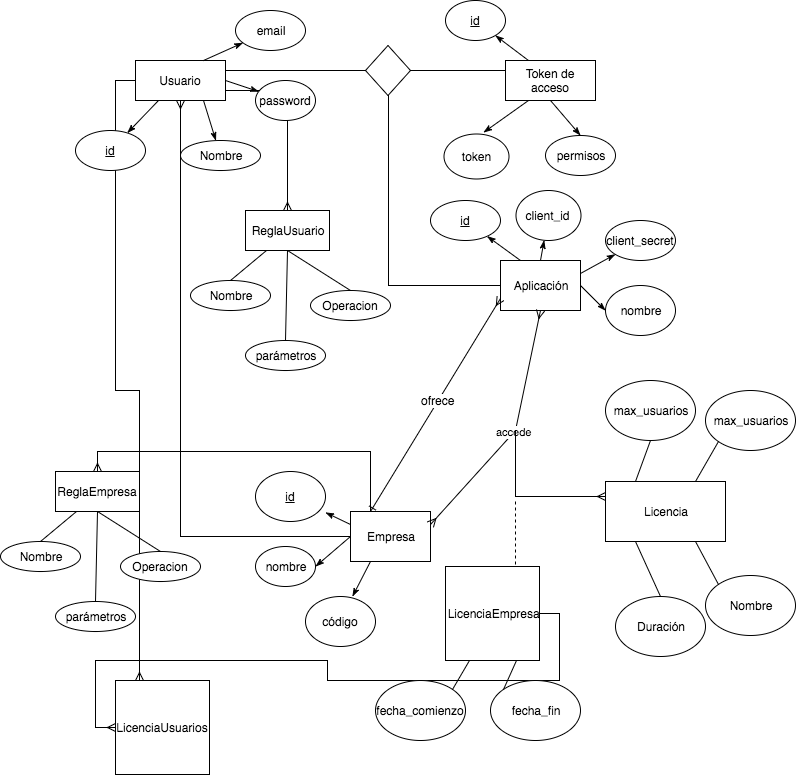
\includegraphics{source/figures/er-model-pfc.png} \ref{modelo_er}

\subsection{Tablas y atributos}\label{tablas-y-atributos}

\subsubsection{Usuarios}\label{usuarios-1}

\begin{longtable}[]{@{}lllll@{}}
\toprule
\begin{minipage}[b]{0.20\columnwidth}\raggedright\strut
Atributos\strut
\end{minipage} & \begin{minipage}[b]{0.18\columnwidth}\raggedright\strut
Tipo\strut
\end{minipage} & \begin{minipage}[b]{0.15\columnwidth}\raggedright\strut
Nulo\strut
\end{minipage} & \begin{minipage}[b]{0.18\columnwidth}\raggedright\strut
Index\strut
\end{minipage} & \begin{minipage}[b]{0.15\columnwidth}\raggedright\strut
Descripción\strut
\end{minipage}\tabularnewline
\midrule
\endhead
\begin{minipage}[t]{0.20\columnwidth}\raggedright\strut
id\strut
\end{minipage} & \begin{minipage}[t]{0.18\columnwidth}\raggedright\strut
INTEGER\strut
\end{minipage} & \begin{minipage}[t]{0.15\columnwidth}\raggedright\strut
NO\strut
\end{minipage} & \begin{minipage}[t]{0.18\columnwidth}\raggedright\strut
PRIMARY\_KEY\strut
\end{minipage} & \begin{minipage}[t]{0.15\columnwidth}\raggedright\strut
Identificador autoincremental\strut
\end{minipage}\tabularnewline
\begin{minipage}[t]{0.20\columnwidth}\raggedright\strut
email\strut
\end{minipage} & \begin{minipage}[t]{0.18\columnwidth}\raggedright\strut
VARCHAR(50)\strut
\end{minipage} & \begin{minipage}[t]{0.15\columnwidth}\raggedright\strut
NO\strut
\end{minipage} & \begin{minipage}[t]{0.18\columnwidth}\raggedright\strut
UNIQUE\strut
\end{minipage} & \begin{minipage}[t]{0.15\columnwidth}\raggedright\strut
Email de usuario, sirve para login\strut
\end{minipage}\tabularnewline
\begin{minipage}[t]{0.20\columnwidth}\raggedright\strut
password\strut
\end{minipage} & \begin{minipage}[t]{0.18\columnwidth}\raggedright\strut
VARCHAR(255)\strut
\end{minipage} & \begin{minipage}[t]{0.15\columnwidth}\raggedright\strut
NO\strut
\end{minipage} & \begin{minipage}[t]{0.18\columnwidth}\raggedright\strut
NO\strut
\end{minipage} & \begin{minipage}[t]{0.15\columnwidth}\raggedright\strut
Password cifrado de usuario\strut
\end{minipage}\tabularnewline
\begin{minipage}[t]{0.20\columnwidth}\raggedright\strut
nombre\strut
\end{minipage} & \begin{minipage}[t]{0.18\columnwidth}\raggedright\strut
VARCHAR(255)\strut
\end{minipage} & \begin{minipage}[t]{0.15\columnwidth}\raggedright\strut
NO\strut
\end{minipage} & \begin{minipage}[t]{0.18\columnwidth}\raggedright\strut
NO\strut
\end{minipage} & \begin{minipage}[t]{0.15\columnwidth}\raggedright\strut
Nombre del usuario\strut
\end{minipage}\tabularnewline
\begin{minipage}[t]{0.20\columnwidth}\raggedright\strut
apellido\strut
\end{minipage} & \begin{minipage}[t]{0.18\columnwidth}\raggedright\strut
VARCHAR(255)\strut
\end{minipage} & \begin{minipage}[t]{0.15\columnwidth}\raggedright\strut
NO\strut
\end{minipage} & \begin{minipage}[t]{0.18\columnwidth}\raggedright\strut
NO\strut
\end{minipage} & \begin{minipage}[t]{0.15\columnwidth}\raggedright\strut
Apellidos del usuario\strut
\end{minipage}\tabularnewline
\begin{minipage}[t]{0.20\columnwidth}\raggedright\strut
company\_id\strut
\end{minipage} & \begin{minipage}[t]{0.18\columnwidth}\raggedright\strut
INTEGER\strut
\end{minipage} & \begin{minipage}[t]{0.15\columnwidth}\raggedright\strut
NO\strut
\end{minipage} & \begin{minipage}[t]{0.18\columnwidth}\raggedright\strut
FOREIGN\_KEY\strut
\end{minipage} & \begin{minipage}[t]{0.15\columnwidth}\raggedright\strut
Id de empresa\strut
\end{minipage}\tabularnewline
\bottomrule
\end{longtable}

\paragraph{Normalización}\label{normalizaciuxf3n}

\begin{itemize}
\tightlist
\item
  La tabla está en primera forma normal ya que:

  \begin{itemize}
  \tightlist
  \item
    Todos los atributos son atómicos.
  \item
    Tiene clave primaria única (id).
  \item
    La CP no puede ser nula.
  \end{itemize}
\item
  La tabla está en segunda forma normal ya que:

  \begin{itemize}
  \tightlist
  \item
    Está en 1FN.
  \item
    Al ser la clave única no puede haber dependencias parciales.
  \end{itemize}
\item
  La tabla está en tercera forma normal ya que:

  \begin{itemize}
  \tightlist
  \item
    Está en 2FN.
  \item
    No hay dependencias funcionales transitivas.
  \end{itemize}
\item
  La tabla está en forma normal de Boyce-Codd ya que:

  \begin{itemize}
  \tightlist
  \item
    Para toda dependencia funcional X-\textgreater{}A X es superllave.
  \end{itemize}
\end{itemize}

\subsubsection{Aplicaciones}\label{aplicaciones-1}

\begin{longtable}[]{@{}lllll@{}}
\toprule
\begin{minipage}[b]{0.21\columnwidth}\raggedright\strut
Atributos\strut
\end{minipage} & \begin{minipage}[b]{0.19\columnwidth}\raggedright\strut
Tipo\strut
\end{minipage} & \begin{minipage}[b]{0.16\columnwidth}\raggedright\strut
Nulo\strut
\end{minipage} & \begin{minipage}[b]{0.19\columnwidth}\raggedright\strut
Index\strut
\end{minipage} & \begin{minipage}[b]{0.11\columnwidth}\raggedright\strut
Descripción\strut
\end{minipage}\tabularnewline
\midrule
\endhead
\begin{minipage}[t]{0.21\columnwidth}\raggedright\strut
id\strut
\end{minipage} & \begin{minipage}[t]{0.19\columnwidth}\raggedright\strut
INTEGER\strut
\end{minipage} & \begin{minipage}[t]{0.16\columnwidth}\raggedright\strut
NO\strut
\end{minipage} & \begin{minipage}[t]{0.19\columnwidth}\raggedright\strut
PRIMARY\_KEY\strut
\end{minipage} & \begin{minipage}[t]{0.11\columnwidth}\raggedright\strut
Identificador autoincremental\strut
\end{minipage}\tabularnewline
\begin{minipage}[t]{0.21\columnwidth}\raggedright\strut
client\_id\strut
\end{minipage} & \begin{minipage}[t]{0.19\columnwidth}\raggedright\strut
VARCHAR(50)\strut
\end{minipage} & \begin{minipage}[t]{0.16\columnwidth}\raggedright\strut
NO\strut
\end{minipage} & \begin{minipage}[t]{0.19\columnwidth}\raggedright\strut
UNIQUE\strut
\end{minipage} & \begin{minipage}[t]{0.11\columnwidth}\raggedright\strut
client id\strut
\end{minipage}\tabularnewline
\begin{minipage}[t]{0.21\columnwidth}\raggedright\strut
client\_secret\strut
\end{minipage} & \begin{minipage}[t]{0.19\columnwidth}\raggedright\strut
VARCHAR(50)\strut
\end{minipage} & \begin{minipage}[t]{0.16\columnwidth}\raggedright\strut
NO\strut
\end{minipage} & \begin{minipage}[t]{0.19\columnwidth}\raggedright\strut
NO\strut
\end{minipage} & \begin{minipage}[t]{0.11\columnwidth}\raggedright\strut
client secret\strut
\end{minipage}\tabularnewline
\begin{minipage}[t]{0.21\columnwidth}\raggedright\strut
name\strut
\end{minipage} & \begin{minipage}[t]{0.19\columnwidth}\raggedright\strut
VARCHAR(50)\strut
\end{minipage} & \begin{minipage}[t]{0.16\columnwidth}\raggedright\strut
NO\strut
\end{minipage} & \begin{minipage}[t]{0.19\columnwidth}\raggedright\strut
NO\strut
\end{minipage} & \begin{minipage}[t]{0.11\columnwidth}\raggedright\strut
Nombre de aplicación\strut
\end{minipage}\tabularnewline
\bottomrule
\end{longtable}

\paragraph{Normalización}\label{normalizaciuxf3n-1}

\begin{itemize}
\tightlist
\item
  La tabla está en primera forma normal ya que:

  \begin{itemize}
  \tightlist
  \item
    Todos los atributos son atómicos.
  \item
    Tiene clave primaria única (id).
  \item
    La CP no puede ser nula.
  \end{itemize}
\item
  La tabla está en segunda forma normal ya que:

  \begin{itemize}
  \tightlist
  \item
    Está en 1FN.
  \item
    Al ser la clave única no puede haber dependencias parciales.
  \end{itemize}
\item
  La tabla está en tercera forma normal ya que:

  \begin{itemize}
  \tightlist
  \item
    Está en 2FN.
  \item
    No hay dependencias funcionales transitivas.
  \end{itemize}
\item
  La tabla está en forma normal de Boyce-Codd ya que:

  \begin{itemize}
  \tightlist
  \item
    Para toda dependencia funcional X-\textgreater{}A X es superllave.
  \end{itemize}
\end{itemize}

\subsubsection{Empresas}\label{empresas-1}

\begin{longtable}[]{@{}lllll@{}}
\toprule
\begin{minipage}[b]{0.21\columnwidth}\raggedright\strut
Atributos\strut
\end{minipage} & \begin{minipage}[b]{0.19\columnwidth}\raggedright\strut
Tipo\strut
\end{minipage} & \begin{minipage}[b]{0.16\columnwidth}\raggedright\strut
Nulo\strut
\end{minipage} & \begin{minipage}[b]{0.19\columnwidth}\raggedright\strut
Index\strut
\end{minipage} & \begin{minipage}[b]{0.11\columnwidth}\raggedright\strut
Descripción\strut
\end{minipage}\tabularnewline
\midrule
\endhead
\begin{minipage}[t]{0.21\columnwidth}\raggedright\strut
id\strut
\end{minipage} & \begin{minipage}[t]{0.19\columnwidth}\raggedright\strut
INTEGER\strut
\end{minipage} & \begin{minipage}[t]{0.16\columnwidth}\raggedright\strut
NO\strut
\end{minipage} & \begin{minipage}[t]{0.19\columnwidth}\raggedright\strut
PRIMARY\_KEY\strut
\end{minipage} & \begin{minipage}[t]{0.11\columnwidth}\raggedright\strut
Identificador autoincremental\strut
\end{minipage}\tabularnewline
\begin{minipage}[t]{0.21\columnwidth}\raggedright\strut
code\strut
\end{minipage} & \begin{minipage}[t]{0.19\columnwidth}\raggedright\strut
VARCHAR(50)\strut
\end{minipage} & \begin{minipage}[t]{0.16\columnwidth}\raggedright\strut
NO\strut
\end{minipage} & \begin{minipage}[t]{0.19\columnwidth}\raggedright\strut
UNIQUE\strut
\end{minipage} & \begin{minipage}[t]{0.11\columnwidth}\raggedright\strut
Código identificador de la empresa\strut
\end{minipage}\tabularnewline
\begin{minipage}[t]{0.21\columnwidth}\raggedright\strut
name\strut
\end{minipage} & \begin{minipage}[t]{0.19\columnwidth}\raggedright\strut
VARCHAR(50)\strut
\end{minipage} & \begin{minipage}[t]{0.16\columnwidth}\raggedright\strut
NO\strut
\end{minipage} & \begin{minipage}[t]{0.19\columnwidth}\raggedright\strut
NO\strut
\end{minipage} & \begin{minipage}[t]{0.11\columnwidth}\raggedright\strut
Nombre de empresa\strut
\end{minipage}\tabularnewline
\bottomrule
\end{longtable}

\paragraph{Normalización}\label{normalizaciuxf3n-2}

\begin{itemize}
\tightlist
\item
  La tabla está en primera forma normal ya que:

  \begin{itemize}
  \tightlist
  \item
    Todos los atributos son atómicos.
  \item
    Tiene clave primaria única (id).
  \item
    La CP no puede ser nula.
  \end{itemize}
\item
  La tabla está en segunda forma normal ya que:

  \begin{itemize}
  \tightlist
  \item
    Está en 1FN.
  \item
    Al ser la clave única no puede haber dependencias parciales.
  \end{itemize}
\item
  La tabla está en tercera forma normal ya que:

  \begin{itemize}
  \tightlist
  \item
    Está en 2FN.
  \item
    No hay dependencias funcionales transitivas.
  \end{itemize}
\item
  La tabla está en forma normal de Boyce-Codd ya que:

  \begin{itemize}
  \tightlist
  \item
    Para toda dependencia funcional X-\textgreater{}A X es superllave.
  \end{itemize}
\end{itemize}

\subsubsection{Tokens de acceso}\label{tokens-de-acceso}

\begin{longtable}[]{@{}lllll@{}}
\toprule
\begin{minipage}[b]{0.21\columnwidth}\raggedright\strut
Atributos\strut
\end{minipage} & \begin{minipage}[b]{0.19\columnwidth}\raggedright\strut
Tipo\strut
\end{minipage} & \begin{minipage}[b]{0.16\columnwidth}\raggedright\strut
Nulo\strut
\end{minipage} & \begin{minipage}[b]{0.19\columnwidth}\raggedright\strut
Index\strut
\end{minipage} & \begin{minipage}[b]{0.11\columnwidth}\raggedright\strut
Descripción\strut
\end{minipage}\tabularnewline
\midrule
\endhead
\begin{minipage}[t]{0.21\columnwidth}\raggedright\strut
id\strut
\end{minipage} & \begin{minipage}[t]{0.19\columnwidth}\raggedright\strut
INTEGER\strut
\end{minipage} & \begin{minipage}[t]{0.16\columnwidth}\raggedright\strut
NO\strut
\end{minipage} & \begin{minipage}[t]{0.19\columnwidth}\raggedright\strut
PRIMARY\_KEY\strut
\end{minipage} & \begin{minipage}[t]{0.11\columnwidth}\raggedright\strut
Identificador autoincremental\strut
\end{minipage}\tabularnewline
\begin{minipage}[t]{0.21\columnwidth}\raggedright\strut
token\strut
\end{minipage} & \begin{minipage}[t]{0.19\columnwidth}\raggedright\strut
VARCHAR(50)\strut
\end{minipage} & \begin{minipage}[t]{0.16\columnwidth}\raggedright\strut
NO\strut
\end{minipage} & \begin{minipage}[t]{0.19\columnwidth}\raggedright\strut
UNIQUE\strut
\end{minipage} & \begin{minipage}[t]{0.11\columnwidth}\raggedright\strut
Token de acceso de usuario\strut
\end{minipage}\tabularnewline
\begin{minipage}[t]{0.21\columnwidth}\raggedright\strut
user\_id\strut
\end{minipage} & \begin{minipage}[t]{0.19\columnwidth}\raggedright\strut
INTEGER\strut
\end{minipage} & \begin{minipage}[t]{0.16\columnwidth}\raggedright\strut
NO\strut
\end{minipage} & \begin{minipage}[t]{0.19\columnwidth}\raggedright\strut
FOREIGN\_KEY\strut
\end{minipage} & \begin{minipage}[t]{0.11\columnwidth}\raggedright\strut
Id de usuario\strut
\end{minipage}\tabularnewline
\begin{minipage}[t]{0.21\columnwidth}\raggedright\strut
application\_id\strut
\end{minipage} & \begin{minipage}[t]{0.19\columnwidth}\raggedright\strut
INTEGER\strut
\end{minipage} & \begin{minipage}[t]{0.16\columnwidth}\raggedright\strut
NO\strut
\end{minipage} & \begin{minipage}[t]{0.19\columnwidth}\raggedright\strut
FOREIGN\_KEY\strut
\end{minipage} & \begin{minipage}[t]{0.11\columnwidth}\raggedright\strut
Id de aplicación\strut
\end{minipage}\tabularnewline
\begin{minipage}[t]{0.21\columnwidth}\raggedright\strut
permisos\strut
\end{minipage} & \begin{minipage}[t]{0.19\columnwidth}\raggedright\strut
VARCHAR(255)\strut
\end{minipage} & \begin{minipage}[t]{0.16\columnwidth}\raggedright\strut
NO\strut
\end{minipage} & \begin{minipage}[t]{0.19\columnwidth}\raggedright\strut
NO\strut
\end{minipage} & \begin{minipage}[t]{0.11\columnwidth}\raggedright\strut
Permisos de token de usuario\strut
\end{minipage}\tabularnewline
\begin{minipage}[t]{0.21\columnwidth}\raggedright\strut
expires\strut
\end{minipage} & \begin{minipage}[t]{0.19\columnwidth}\raggedright\strut
INTEGER\strut
\end{minipage} & \begin{minipage}[t]{0.16\columnwidth}\raggedright\strut
NO\strut
\end{minipage} & \begin{minipage}[t]{0.19\columnwidth}\raggedright\strut
NO\strut
\end{minipage} & \begin{minipage}[t]{0.11\columnwidth}\raggedright\strut
Segundos de expiración de token\strut
\end{minipage}\tabularnewline
\bottomrule
\end{longtable}

\paragraph{Normalización}\label{normalizaciuxf3n-3}

\begin{itemize}
\tightlist
\item
  La tabla está en primera forma normal ya que:

  \begin{itemize}
  \tightlist
  \item
    Todos los atributos son atómicos.
  \item
    Tiene clave primaria única (id).
  \item
    La CP no puede ser nula.
  \end{itemize}
\item
  La tabla está en segunda forma normal ya que:

  \begin{itemize}
  \tightlist
  \item
    Está en 1FN.
  \item
    Al ser la clave única no puede haber dependencias parciales.
  \end{itemize}
\item
  La tabla está en tercera forma normal ya que:

  \begin{itemize}
  \tightlist
  \item
    Está en 2FN.
  \item
    No hay dependencias funcionales transitivas.
  \end{itemize}
\item
  La tabla está en forma normal de Boyce-Codd ya que:

  \begin{itemize}
  \tightlist
  \item
    Para toda dependencia funcional X-\textgreater{}A X es superllave.
  \end{itemize}
\end{itemize}

\subsubsection{Refresh tokens}\label{refresh-tokens}

\begin{longtable}[]{@{}lllll@{}}
\toprule
\begin{minipage}[b]{0.21\columnwidth}\raggedright\strut
Atributos\strut
\end{minipage} & \begin{minipage}[b]{0.19\columnwidth}\raggedright\strut
Tipo\strut
\end{minipage} & \begin{minipage}[b]{0.16\columnwidth}\raggedright\strut
Nulo\strut
\end{minipage} & \begin{minipage}[b]{0.19\columnwidth}\raggedright\strut
Index\strut
\end{minipage} & \begin{minipage}[b]{0.11\columnwidth}\raggedright\strut
Descripción\strut
\end{minipage}\tabularnewline
\midrule
\endhead
\begin{minipage}[t]{0.21\columnwidth}\raggedright\strut
id\strut
\end{minipage} & \begin{minipage}[t]{0.19\columnwidth}\raggedright\strut
INTEGER\strut
\end{minipage} & \begin{minipage}[t]{0.16\columnwidth}\raggedright\strut
NO\strut
\end{minipage} & \begin{minipage}[t]{0.19\columnwidth}\raggedright\strut
PRIMARY\_KEY\strut
\end{minipage} & \begin{minipage}[t]{0.11\columnwidth}\raggedright\strut
Identificador autoincremental\strut
\end{minipage}\tabularnewline
\begin{minipage}[t]{0.21\columnwidth}\raggedright\strut
token\strut
\end{minipage} & \begin{minipage}[t]{0.19\columnwidth}\raggedright\strut
VARCHAR(50)\strut
\end{minipage} & \begin{minipage}[t]{0.16\columnwidth}\raggedright\strut
NO\strut
\end{minipage} & \begin{minipage}[t]{0.19\columnwidth}\raggedright\strut
UNIQUE\strut
\end{minipage} & \begin{minipage}[t]{0.11\columnwidth}\raggedright\strut
Token de refresco de usuario\strut
\end{minipage}\tabularnewline
\begin{minipage}[t]{0.21\columnwidth}\raggedright\strut
access\_token\_id\strut
\end{minipage} & \begin{minipage}[t]{0.19\columnwidth}\raggedright\strut
INTEGER\strut
\end{minipage} & \begin{minipage}[t]{0.16\columnwidth}\raggedright\strut
NO\strut
\end{minipage} & \begin{minipage}[t]{0.19\columnwidth}\raggedright\strut
FOREIGN\_KEY\strut
\end{minipage} & \begin{minipage}[t]{0.11\columnwidth}\raggedright\strut
Id de usuario\strut
\end{minipage}\tabularnewline
\bottomrule
\end{longtable}

\paragraph{Normalización}\label{normalizaciuxf3n-4}

\begin{itemize}
\tightlist
\item
  La tabla está en primera forma normal ya que:

  \begin{itemize}
  \tightlist
  \item
    Todos los atributos son atómicos.
  \item
    Tiene clave primaria única (id).
  \item
    La CP no puede ser nula.
  \end{itemize}
\item
  La tabla está en segunda forma normal ya que:

  \begin{itemize}
  \tightlist
  \item
    Está en 1FN.
  \item
    Al ser la clave única no puede haber dependencias parciales.
  \end{itemize}
\item
  La tabla está en tercera forma normal ya que:

  \begin{itemize}
  \tightlist
  \item
    Está en 2FN.
  \item
    No hay dependencias funcionales transitivas.
  \end{itemize}
\item
  La tabla está en forma normal de Boyce-Codd ya que:

  \begin{itemize}
  \tightlist
  \item
    Para toda dependencia funcional X-\textgreater{}A X es superllave.
  \end{itemize}
\end{itemize}

\subsubsection{Authorization codes}\label{authorization-codes}

\begin{longtable}[]{@{}lllll@{}}
\toprule
\begin{minipage}[b]{0.21\columnwidth}\raggedright\strut
Atributos\strut
\end{minipage} & \begin{minipage}[b]{0.19\columnwidth}\raggedright\strut
Tipo\strut
\end{minipage} & \begin{minipage}[b]{0.16\columnwidth}\raggedright\strut
Nulo\strut
\end{minipage} & \begin{minipage}[b]{0.19\columnwidth}\raggedright\strut
Index\strut
\end{minipage} & \begin{minipage}[b]{0.11\columnwidth}\raggedright\strut
Descripción\strut
\end{minipage}\tabularnewline
\midrule
\endhead
\begin{minipage}[t]{0.21\columnwidth}\raggedright\strut
id\strut
\end{minipage} & \begin{minipage}[t]{0.19\columnwidth}\raggedright\strut
INTEGER\strut
\end{minipage} & \begin{minipage}[t]{0.16\columnwidth}\raggedright\strut
NO\strut
\end{minipage} & \begin{minipage}[t]{0.19\columnwidth}\raggedright\strut
PRIMARY\_KEY\strut
\end{minipage} & \begin{minipage}[t]{0.11\columnwidth}\raggedright\strut
Identificador autoincremental\strut
\end{minipage}\tabularnewline
\begin{minipage}[t]{0.21\columnwidth}\raggedright\strut
code\strut
\end{minipage} & \begin{minipage}[t]{0.19\columnwidth}\raggedright\strut
VARCHAR(50)\strut
\end{minipage} & \begin{minipage}[t]{0.16\columnwidth}\raggedright\strut
NO\strut
\end{minipage} & \begin{minipage}[t]{0.19\columnwidth}\raggedright\strut
UNIQUE\strut
\end{minipage} & \begin{minipage}[t]{0.11\columnwidth}\raggedright\strut
Código de autorización\strut
\end{minipage}\tabularnewline
\begin{minipage}[t]{0.21\columnwidth}\raggedright\strut
application\_id\strut
\end{minipage} & \begin{minipage}[t]{0.19\columnwidth}\raggedright\strut
INTEGER\strut
\end{minipage} & \begin{minipage}[t]{0.16\columnwidth}\raggedright\strut
NO\strut
\end{minipage} & \begin{minipage}[t]{0.19\columnwidth}\raggedright\strut
FOREIGN\_KEY\strut
\end{minipage} & \begin{minipage}[t]{0.11\columnwidth}\raggedright\strut
Id de usuario\strut
\end{minipage}\tabularnewline
\begin{minipage}[t]{0.21\columnwidth}\raggedright\strut
user\_id\strut
\end{minipage} & \begin{minipage}[t]{0.19\columnwidth}\raggedright\strut
INTEGER\strut
\end{minipage} & \begin{minipage}[t]{0.16\columnwidth}\raggedright\strut
NO\strut
\end{minipage} & \begin{minipage}[t]{0.19\columnwidth}\raggedright\strut
FOREIGN\_KEY\strut
\end{minipage} & \begin{minipage}[t]{0.11\columnwidth}\raggedright\strut
Id de usuario\strut
\end{minipage}\tabularnewline
\begin{minipage}[t]{0.21\columnwidth}\raggedright\strut
expires\strut
\end{minipage} & \begin{minipage}[t]{0.19\columnwidth}\raggedright\strut
INTEGER\strut
\end{minipage} & \begin{minipage}[t]{0.16\columnwidth}\raggedright\strut
NO\strut
\end{minipage} & \begin{minipage}[t]{0.19\columnwidth}\raggedright\strut
NO\strut
\end{minipage} & \begin{minipage}[t]{0.11\columnwidth}\raggedright\strut
Segundos de expiración de token\strut
\end{minipage}\tabularnewline
\bottomrule
\end{longtable}

\paragraph{Normalización}\label{normalizaciuxf3n-5}

\begin{itemize}
\tightlist
\item
  La tabla está en primera forma normal ya que:

  \begin{itemize}
  \tightlist
  \item
    Todos los atributos son atómicos.
  \item
    Tiene clave primaria única (id).
  \item
    La CP no puede ser nula.
  \end{itemize}
\item
  La tabla está en segunda forma normal ya que:

  \begin{itemize}
  \tightlist
  \item
    Está en 1FN.
  \item
    Al ser la clave única no puede haber dependencias parciales.
  \end{itemize}
\item
  La tabla está en tercera forma normal ya que:

  \begin{itemize}
  \tightlist
  \item
    Está en 2FN.
  \item
    No hay dependencias funcionales transitivas.
  \end{itemize}
\item
  La tabla está en forma normal de Boyce-Codd ya que:

  \begin{itemize}
  \tightlist
  \item
    Para toda dependencia funcional X-\textgreater{}A X es superllave.
  \end{itemize}
\end{itemize}

\subsubsection{Token de refresco}\label{token-de-refresco}

\begin{longtable}[]{@{}lllll@{}}
\toprule
\begin{minipage}[b]{0.21\columnwidth}\raggedright\strut
Atributos\strut
\end{minipage} & \begin{minipage}[b]{0.19\columnwidth}\raggedright\strut
Tipo\strut
\end{minipage} & \begin{minipage}[b]{0.16\columnwidth}\raggedright\strut
Nulo\strut
\end{minipage} & \begin{minipage}[b]{0.19\columnwidth}\raggedright\strut
Index\strut
\end{minipage} & \begin{minipage}[b]{0.11\columnwidth}\raggedright\strut
Descripción\strut
\end{minipage}\tabularnewline
\midrule
\endhead
\begin{minipage}[t]{0.21\columnwidth}\raggedright\strut
id\strut
\end{minipage} & \begin{minipage}[t]{0.19\columnwidth}\raggedright\strut
INTEGER\strut
\end{minipage} & \begin{minipage}[t]{0.16\columnwidth}\raggedright\strut
NO\strut
\end{minipage} & \begin{minipage}[t]{0.19\columnwidth}\raggedright\strut
PRIMARY\_KEY\strut
\end{minipage} & \begin{minipage}[t]{0.11\columnwidth}\raggedright\strut
Identificador autoincremental\strut
\end{minipage}\tabularnewline
\begin{minipage}[t]{0.21\columnwidth}\raggedright\strut
token\strut
\end{minipage} & \begin{minipage}[t]{0.19\columnwidth}\raggedright\strut
VARCHAR(50)\strut
\end{minipage} & \begin{minipage}[t]{0.16\columnwidth}\raggedright\strut
NO\strut
\end{minipage} & \begin{minipage}[t]{0.19\columnwidth}\raggedright\strut
UNIQUE\strut
\end{minipage} & \begin{minipage}[t]{0.11\columnwidth}\raggedright\strut
Token de refresco\strut
\end{minipage}\tabularnewline
\begin{minipage}[t]{0.21\columnwidth}\raggedright\strut
access\_token\_id\strut
\end{minipage} & \begin{minipage}[t]{0.19\columnwidth}\raggedright\strut
INTEGER\strut
\end{minipage} & \begin{minipage}[t]{0.16\columnwidth}\raggedright\strut
NO\strut
\end{minipage} & \begin{minipage}[t]{0.19\columnwidth}\raggedright\strut
FOREIGN\_KEY\strut
\end{minipage} & \begin{minipage}[t]{0.11\columnwidth}\raggedright\strut
Id del token de acceso\strut
\end{minipage}\tabularnewline
\bottomrule
\end{longtable}

\paragraph{Normalización}\label{normalizaciuxf3n-6}

\begin{itemize}
\tightlist
\item
  La tabla está en primera forma normal ya que:

  \begin{itemize}
  \tightlist
  \item
    Todos los atributos son atómicos.
  \item
    Tiene clave primaria única (id).
  \item
    La CP no puede ser nula.
  \end{itemize}
\item
  La tabla está en segunda forma normal ya que:

  \begin{itemize}
  \tightlist
  \item
    Está en 1FN.
  \item
    Al ser la clave única no puede haber dependencias parciales.
  \end{itemize}
\item
  La tabla está en tercera forma normal ya que:

  \begin{itemize}
  \tightlist
  \item
    Está en 2FN.
  \item
    No hay dependencias funcionales transitivas.
  \end{itemize}
\item
  La tabla está en forma normal de Boyce-Codd ya que:

  \begin{itemize}
  \tightlist
  \item
    Para toda dependencia funcional X-\textgreater{}A X es superllave.
  \end{itemize}
\end{itemize}

\subsubsection{Licencia}\label{licencia}

\begin{longtable}[]{@{}lllll@{}}
\toprule
\begin{minipage}[b]{0.21\columnwidth}\raggedright\strut
Atributos\strut
\end{minipage} & \begin{minipage}[b]{0.19\columnwidth}\raggedright\strut
Tipo\strut
\end{minipage} & \begin{minipage}[b]{0.16\columnwidth}\raggedright\strut
Nulo\strut
\end{minipage} & \begin{minipage}[b]{0.19\columnwidth}\raggedright\strut
Index\strut
\end{minipage} & \begin{minipage}[b]{0.11\columnwidth}\raggedright\strut
Descripción\strut
\end{minipage}\tabularnewline
\midrule
\endhead
\begin{minipage}[t]{0.21\columnwidth}\raggedright\strut
id\strut
\end{minipage} & \begin{minipage}[t]{0.19\columnwidth}\raggedright\strut
INTEGER\strut
\end{minipage} & \begin{minipage}[t]{0.16\columnwidth}\raggedright\strut
NO\strut
\end{minipage} & \begin{minipage}[t]{0.19\columnwidth}\raggedright\strut
PRIMARY\_KEY\strut
\end{minipage} & \begin{minipage}[t]{0.11\columnwidth}\raggedright\strut
Identificador autoincremental\strut
\end{minipage}\tabularnewline
\begin{minipage}[t]{0.21\columnwidth}\raggedright\strut
name\strut
\end{minipage} & \begin{minipage}[t]{0.19\columnwidth}\raggedright\strut
VARCHAR(50)\strut
\end{minipage} & \begin{minipage}[t]{0.16\columnwidth}\raggedright\strut
NO\strut
\end{minipage} & \begin{minipage}[t]{0.19\columnwidth}\raggedright\strut
UNIQUE\strut
\end{minipage} & \begin{minipage}[t]{0.11\columnwidth}\raggedright\strut
Nombre de la licencia\strut
\end{minipage}\tabularnewline
\begin{minipage}[t]{0.21\columnwidth}\raggedright\strut
duration\_days\strut
\end{minipage} & \begin{minipage}[t]{0.19\columnwidth}\raggedright\strut
INTEGER\strut
\end{minipage} & \begin{minipage}[t]{0.16\columnwidth}\raggedright\strut
NO\strut
\end{minipage} & \begin{minipage}[t]{0.19\columnwidth}\raggedright\strut
NO\strut
\end{minipage} & \begin{minipage}[t]{0.11\columnwidth}\raggedright\strut
Duración en días de la licencia\strut
\end{minipage}\tabularnewline
\begin{minipage}[t]{0.21\columnwidth}\raggedright\strut
max\_users\strut
\end{minipage} & \begin{minipage}[t]{0.19\columnwidth}\raggedright\strut
INTEGER\strut
\end{minipage} & \begin{minipage}[t]{0.16\columnwidth}\raggedright\strut
NO\strut
\end{minipage} & \begin{minipage}[t]{0.19\columnwidth}\raggedright\strut
NO\strut
\end{minipage} & \begin{minipage}[t]{0.11\columnwidth}\raggedright\strut
Número máximo de usuarios que permite esta licencia\strut
\end{minipage}\tabularnewline
\bottomrule
\end{longtable}

\paragraph{Normalización}\label{normalizaciuxf3n-7}

\begin{itemize}
\tightlist
\item
  La tabla está en primera forma normal ya que:

  \begin{itemize}
  \tightlist
  \item
    Todos los atributos son atómicos.
  \item
    Tiene clave primaria única (id).
  \item
    La CP no puede ser nula.
  \end{itemize}
\item
  La tabla está en segunda forma normal ya que:

  \begin{itemize}
  \tightlist
  \item
    Está en 1FN.
  \item
    Al ser la clave única no puede haber dependencias parciales.
  \end{itemize}
\item
  La tabla está en tercera forma normal ya que:

  \begin{itemize}
  \tightlist
  \item
    Está en 2FN.
  \item
    No hay dependencias funcionales transitivas.
  \end{itemize}
\item
  La tabla está en forma normal de Boyce-Codd ya que:

  \begin{itemize}
  \tightlist
  \item
    Para toda dependencia funcional X-\textgreater{}A X es superllave.
  \end{itemize}
\end{itemize}

\subsubsection{LicenciaEmpresa}\label{licenciaempresa}

\begin{longtable}[]{@{}lllll@{}}
\toprule
\begin{minipage}[b]{0.21\columnwidth}\raggedright\strut
Atributos\strut
\end{minipage} & \begin{minipage}[b]{0.19\columnwidth}\raggedright\strut
Tipo\strut
\end{minipage} & \begin{minipage}[b]{0.16\columnwidth}\raggedright\strut
Nulo\strut
\end{minipage} & \begin{minipage}[b]{0.19\columnwidth}\raggedright\strut
Index\strut
\end{minipage} & \begin{minipage}[b]{0.11\columnwidth}\raggedright\strut
Descripción\strut
\end{minipage}\tabularnewline
\midrule
\endhead
\begin{minipage}[t]{0.21\columnwidth}\raggedright\strut
id\strut
\end{minipage} & \begin{minipage}[t]{0.19\columnwidth}\raggedright\strut
INTEGER\strut
\end{minipage} & \begin{minipage}[t]{0.16\columnwidth}\raggedright\strut
NO\strut
\end{minipage} & \begin{minipage}[t]{0.19\columnwidth}\raggedright\strut
PRIMARY\_KEY\strut
\end{minipage} & \begin{minipage}[t]{0.11\columnwidth}\raggedright\strut
Identificador autoincremental\strut
\end{minipage}\tabularnewline
\begin{minipage}[t]{0.21\columnwidth}\raggedright\strut
license\_id\strut
\end{minipage} & \begin{minipage}[t]{0.19\columnwidth}\raggedright\strut
INTEGER\strut
\end{minipage} & \begin{minipage}[t]{0.16\columnwidth}\raggedright\strut
NO\strut
\end{minipage} & \begin{minipage}[t]{0.19\columnwidth}\raggedright\strut
FOREIGN\_KEY\strut
\end{minipage} & \begin{minipage}[t]{0.11\columnwidth}\raggedright\strut
Id de licencia\strut
\end{minipage}\tabularnewline
\begin{minipage}[t]{0.21\columnwidth}\raggedright\strut
company\_id\strut
\end{minipage} & \begin{minipage}[t]{0.19\columnwidth}\raggedright\strut
INTEGER\strut
\end{minipage} & \begin{minipage}[t]{0.16\columnwidth}\raggedright\strut
NO\strut
\end{minipage} & \begin{minipage}[t]{0.19\columnwidth}\raggedright\strut
FOREIGN\_KEY\strut
\end{minipage} & \begin{minipage}[t]{0.11\columnwidth}\raggedright\strut
Id de la empresa\strut
\end{minipage}\tabularnewline
\begin{minipage}[t]{0.21\columnwidth}\raggedright\strut
start\_date\strut
\end{minipage} & \begin{minipage}[t]{0.19\columnwidth}\raggedright\strut
DATETIME\strut
\end{minipage} & \begin{minipage}[t]{0.16\columnwidth}\raggedright\strut
NO\strut
\end{minipage} & \begin{minipage}[t]{0.19\columnwidth}\raggedright\strut
NO\strut
\end{minipage} & \begin{minipage}[t]{0.11\columnwidth}\raggedright\strut
Fecha de comienzo de la licencia\strut
\end{minipage}\tabularnewline
\begin{minipage}[t]{0.21\columnwidth}\raggedright\strut
end\_date\strut
\end{minipage} & \begin{minipage}[t]{0.19\columnwidth}\raggedright\strut
DATETIME\strut
\end{minipage} & \begin{minipage}[t]{0.16\columnwidth}\raggedright\strut
NO\strut
\end{minipage} & \begin{minipage}[t]{0.19\columnwidth}\raggedright\strut
NO\strut
\end{minipage} & \begin{minipage}[t]{0.11\columnwidth}\raggedright\strut
Fecha de comienzo de la licencia\strut
\end{minipage}\tabularnewline
\bottomrule
\end{longtable}

\paragraph{Normalización}\label{normalizaciuxf3n-8}

\begin{itemize}
\tightlist
\item
  La tabla está en primera forma normal ya que:

  \begin{itemize}
  \tightlist
  \item
    Todos los atributos son atómicos.
  \item
    Tiene clave primaria única (id).
  \item
    La CP no puede ser nula.
  \end{itemize}
\item
  La tabla está en segunda forma normal ya que:

  \begin{itemize}
  \tightlist
  \item
    Está en 1FN.
  \item
    Al ser la clave única no puede haber dependencias parciales.
  \end{itemize}
\item
  La tabla está en tercera forma normal ya que:

  \begin{itemize}
  \tightlist
  \item
    Está en 2FN.
  \item
    No hay dependencias funcionales transitivas.
  \end{itemize}
\item
  La tabla está en forma normal de Boyce-Codd ya que:

  \begin{itemize}
  \tightlist
  \item
    Para toda dependencia funcional X-\textgreater{}A X es superllave.
  \end{itemize}
\end{itemize}

\subsubsection{ConfiguracionGlobal}\label{configuracionglobal}

\begin{longtable}[]{@{}lllll@{}}
\toprule
\begin{minipage}[b]{0.21\columnwidth}\raggedright\strut
Atributos\strut
\end{minipage} & \begin{minipage}[b]{0.19\columnwidth}\raggedright\strut
Tipo\strut
\end{minipage} & \begin{minipage}[b]{0.16\columnwidth}\raggedright\strut
Nulo\strut
\end{minipage} & \begin{minipage}[b]{0.19\columnwidth}\raggedright\strut
Index\strut
\end{minipage} & \begin{minipage}[b]{0.11\columnwidth}\raggedright\strut
Descripción\strut
\end{minipage}\tabularnewline
\midrule
\endhead
\begin{minipage}[t]{0.21\columnwidth}\raggedright\strut
id\strut
\end{minipage} & \begin{minipage}[t]{0.19\columnwidth}\raggedright\strut
INTEGER\strut
\end{minipage} & \begin{minipage}[t]{0.16\columnwidth}\raggedright\strut
NO\strut
\end{minipage} & \begin{minipage}[t]{0.19\columnwidth}\raggedright\strut
PRIMARY\_KEY\strut
\end{minipage} & \begin{minipage}[t]{0.11\columnwidth}\raggedright\strut
Identificador autoincremental\strut
\end{minipage}\tabularnewline
\begin{minipage}[t]{0.21\columnwidth}\raggedright\strut
application\_id\strut
\end{minipage} & \begin{minipage}[t]{0.19\columnwidth}\raggedright\strut
INTEGER\strut
\end{minipage} & \begin{minipage}[t]{0.16\columnwidth}\raggedright\strut
NO\strut
\end{minipage} & \begin{minipage}[t]{0.19\columnwidth}\raggedright\strut
FOREIGN\_KEY\strut
\end{minipage} & \begin{minipage}[t]{0.11\columnwidth}\raggedright\strut
Id de aplicación\strut
\end{minipage}\tabularnewline
\begin{minipage}[t]{0.21\columnwidth}\raggedright\strut
key\strut
\end{minipage} & \begin{minipage}[t]{0.19\columnwidth}\raggedright\strut
VARCHAR(50)\strut
\end{minipage} & \begin{minipage}[t]{0.16\columnwidth}\raggedright\strut
NO\strut
\end{minipage} & \begin{minipage}[t]{0.19\columnwidth}\raggedright\strut
NO\strut
\end{minipage} & \begin{minipage}[t]{0.11\columnwidth}\raggedright\strut
Clave de configuración\strut
\end{minipage}\tabularnewline
\begin{minipage}[t]{0.21\columnwidth}\raggedright\strut
value\strut
\end{minipage} & \begin{minipage}[t]{0.19\columnwidth}\raggedright\strut
VARCHAR(50)\strut
\end{minipage} & \begin{minipage}[t]{0.16\columnwidth}\raggedright\strut
NO\strut
\end{minipage} & \begin{minipage}[t]{0.19\columnwidth}\raggedright\strut
NO\strut
\end{minipage} & \begin{minipage}[t]{0.11\columnwidth}\raggedright\strut
Valor de configuración\strut
\end{minipage}\tabularnewline
\bottomrule
\end{longtable}

\paragraph{Normalización}\label{normalizaciuxf3n-9}

\begin{itemize}
\tightlist
\item
  La tabla está en primera forma normal ya que:

  \begin{itemize}
  \tightlist
  \item
    Todos los atributos son atómicos.
  \item
    Tiene clave primaria única (id).
  \item
    La CP no puede ser nula.
  \end{itemize}
\item
  La tabla está en segunda forma normal ya que:

  \begin{itemize}
  \tightlist
  \item
    Está en 1FN.
  \item
    Al ser la clave única no puede haber dependencias parciales.
  \end{itemize}
\item
  La tabla está en tercera forma normal ya que:

  \begin{itemize}
  \tightlist
  \item
    Está en 2FN.
  \item
    No hay dependencias funcionales transitivas.
  \end{itemize}
\item
  La tabla está en forma normal de Boyce-Codd ya que:

  \begin{itemize}
  \tightlist
  \item
    Para toda dependencia funcional X-\textgreater{}A X es superllave.
  \end{itemize}
\end{itemize}

\subsubsection{ConfiguracionEmpresa}\label{configuracionempresa}

\begin{longtable}[]{@{}lllll@{}}
\toprule
\begin{minipage}[b]{0.21\columnwidth}\raggedright\strut
Atributos\strut
\end{minipage} & \begin{minipage}[b]{0.19\columnwidth}\raggedright\strut
Tipo\strut
\end{minipage} & \begin{minipage}[b]{0.16\columnwidth}\raggedright\strut
Nulo\strut
\end{minipage} & \begin{minipage}[b]{0.19\columnwidth}\raggedright\strut
Index\strut
\end{minipage} & \begin{minipage}[b]{0.11\columnwidth}\raggedright\strut
Descripción\strut
\end{minipage}\tabularnewline
\midrule
\endhead
\begin{minipage}[t]{0.21\columnwidth}\raggedright\strut
id\strut
\end{minipage} & \begin{minipage}[t]{0.19\columnwidth}\raggedright\strut
INTEGER\strut
\end{minipage} & \begin{minipage}[t]{0.16\columnwidth}\raggedright\strut
NO\strut
\end{minipage} & \begin{minipage}[t]{0.19\columnwidth}\raggedright\strut
PRIMARY\_KEY\strut
\end{minipage} & \begin{minipage}[t]{0.11\columnwidth}\raggedright\strut
Identificador autoincremental\strut
\end{minipage}\tabularnewline
\begin{minipage}[t]{0.21\columnwidth}\raggedright\strut
application\_id\strut
\end{minipage} & \begin{minipage}[t]{0.19\columnwidth}\raggedright\strut
INTEGER\strut
\end{minipage} & \begin{minipage}[t]{0.16\columnwidth}\raggedright\strut
NO\strut
\end{minipage} & \begin{minipage}[t]{0.19\columnwidth}\raggedright\strut
FOREIGN\_KEY\strut
\end{minipage} & \begin{minipage}[t]{0.11\columnwidth}\raggedright\strut
Id de aplicación\strut
\end{minipage}\tabularnewline
\begin{minipage}[t]{0.21\columnwidth}\raggedright\strut
company\_id\strut
\end{minipage} & \begin{minipage}[t]{0.19\columnwidth}\raggedright\strut
INTEGER\strut
\end{minipage} & \begin{minipage}[t]{0.16\columnwidth}\raggedright\strut
NO\strut
\end{minipage} & \begin{minipage}[t]{0.19\columnwidth}\raggedright\strut
FOREIGN\_KEY\strut
\end{minipage} & \begin{minipage}[t]{0.11\columnwidth}\raggedright\strut
Id de empresa\strut
\end{minipage}\tabularnewline
\begin{minipage}[t]{0.21\columnwidth}\raggedright\strut
key\strut
\end{minipage} & \begin{minipage}[t]{0.19\columnwidth}\raggedright\strut
VARCHAR(50)\strut
\end{minipage} & \begin{minipage}[t]{0.16\columnwidth}\raggedright\strut
NO\strut
\end{minipage} & \begin{minipage}[t]{0.19\columnwidth}\raggedright\strut
NO\strut
\end{minipage} & \begin{minipage}[t]{0.11\columnwidth}\raggedright\strut
Clave de configuración\strut
\end{minipage}\tabularnewline
\begin{minipage}[t]{0.21\columnwidth}\raggedright\strut
value\strut
\end{minipage} & \begin{minipage}[t]{0.19\columnwidth}\raggedright\strut
VARCHAR(50)\strut
\end{minipage} & \begin{minipage}[t]{0.16\columnwidth}\raggedright\strut
NO\strut
\end{minipage} & \begin{minipage}[t]{0.19\columnwidth}\raggedright\strut
NO\strut
\end{minipage} & \begin{minipage}[t]{0.11\columnwidth}\raggedright\strut
Valor de configuración\strut
\end{minipage}\tabularnewline
\bottomrule
\end{longtable}

\paragraph{Normalización}\label{normalizaciuxf3n-10}

\begin{itemize}
\tightlist
\item
  La tabla está en primera forma normal ya que:

  \begin{itemize}
  \tightlist
  \item
    Todos los atributos son atómicos.
  \item
    Tiene clave primaria única (id).
  \item
    La CP no puede ser nula.
  \end{itemize}
\item
  La tabla está en segunda forma normal ya que:

  \begin{itemize}
  \tightlist
  \item
    Está en 1FN.
  \item
    Al ser la clave única no puede haber dependencias parciales.
  \end{itemize}
\item
  La tabla está en tercera forma normal ya que:

  \begin{itemize}
  \tightlist
  \item
    Está en 2FN.
  \item
    No hay dependencias funcionales transitivas.
  \end{itemize}
\item
  La tabla está en forma normal de Boyce-Codd ya que:

  \begin{itemize}
  \tightlist
  \item
    Para toda dependencia funcional X-\textgreater{}A X es superllave.
  \end{itemize}
\end{itemize}

\subsubsection{ReglaUsuario}\label{reglausuario}

\begin{longtable}[]{@{}lllll@{}}
\toprule
\begin{minipage}[b]{0.21\columnwidth}\raggedright\strut
Atributos\strut
\end{minipage} & \begin{minipage}[b]{0.19\columnwidth}\raggedright\strut
Tipo\strut
\end{minipage} & \begin{minipage}[b]{0.16\columnwidth}\raggedright\strut
Nulo\strut
\end{minipage} & \begin{minipage}[b]{0.19\columnwidth}\raggedright\strut
Index\strut
\end{minipage} & \begin{minipage}[b]{0.11\columnwidth}\raggedright\strut
Descripción\strut
\end{minipage}\tabularnewline
\midrule
\endhead
\begin{minipage}[t]{0.21\columnwidth}\raggedright\strut
id\strut
\end{minipage} & \begin{minipage}[t]{0.19\columnwidth}\raggedright\strut
INTEGER\strut
\end{minipage} & \begin{minipage}[t]{0.16\columnwidth}\raggedright\strut
NO\strut
\end{minipage} & \begin{minipage}[t]{0.19\columnwidth}\raggedright\strut
PRIMARY\_KEY\strut
\end{minipage} & \begin{minipage}[t]{0.11\columnwidth}\raggedright\strut
Identificador autoincremental\strut
\end{minipage}\tabularnewline
\begin{minipage}[t]{0.21\columnwidth}\raggedright\strut
user\_id\strut
\end{minipage} & \begin{minipage}[t]{0.19\columnwidth}\raggedright\strut
INTEGER\strut
\end{minipage} & \begin{minipage}[t]{0.16\columnwidth}\raggedright\strut
NO\strut
\end{minipage} & \begin{minipage}[t]{0.19\columnwidth}\raggedright\strut
FOREIGN\_KEY\strut
\end{minipage} & \begin{minipage}[t]{0.11\columnwidth}\raggedright\strut
Id de usuario\strut
\end{minipage}\tabularnewline
\begin{minipage}[t]{0.21\columnwidth}\raggedright\strut
operación\strut
\end{minipage} & \begin{minipage}[t]{0.19\columnwidth}\raggedright\strut
VARCHAR(50)\strut
\end{minipage} & \begin{minipage}[t]{0.16\columnwidth}\raggedright\strut
NO\strut
\end{minipage} & \begin{minipage}[t]{0.19\columnwidth}\raggedright\strut
NO\strut
\end{minipage} & \begin{minipage}[t]{0.11\columnwidth}\raggedright\strut
Nombre de operación a aplicar\strut
\end{minipage}\tabularnewline
\begin{minipage}[t]{0.21\columnwidth}\raggedright\strut
parámetro\strut
\end{minipage} & \begin{minipage}[t]{0.19\columnwidth}\raggedright\strut
VARCHAR(50)\strut
\end{minipage} & \begin{minipage}[t]{0.16\columnwidth}\raggedright\strut
NO\strut
\end{minipage} & \begin{minipage}[t]{0.19\columnwidth}\raggedright\strut
NO\strut
\end{minipage} & \begin{minipage}[t]{0.11\columnwidth}\raggedright\strut
Parámetro a operar\strut
\end{minipage}\tabularnewline
\bottomrule
\end{longtable}

\paragraph{Normalización}\label{normalizaciuxf3n-11}

\begin{itemize}
\tightlist
\item
  La tabla está en primera forma normal ya que:

  \begin{itemize}
  \tightlist
  \item
    Todos los atributos son atómicos.
  \item
    Tiene clave primaria única (id).
  \item
    La CP no puede ser nula.
  \end{itemize}
\item
  La tabla está en segunda forma normal ya que:

  \begin{itemize}
  \tightlist
  \item
    Está en 1FN.
  \item
    Al ser la clave única no puede haber dependencias parciales.
  \end{itemize}
\item
  La tabla está en tercera forma normal ya que:

  \begin{itemize}
  \tightlist
  \item
    Está en 2FN.
  \item
    No hay dependencias funcionales transitivas.
  \end{itemize}
\item
  La tabla está en forma normal de Boyce-Codd ya que:

  \begin{itemize}
  \tightlist
  \item
    Para toda dependencia funcional X-\textgreater{}A X es superllave.
  \end{itemize}
\end{itemize}

\subsubsection{ReglaEmpresa}\label{reglaempresa}

\begin{longtable}[]{@{}lllll@{}}
\toprule
\begin{minipage}[b]{0.21\columnwidth}\raggedright\strut
Atributos\strut
\end{minipage} & \begin{minipage}[b]{0.19\columnwidth}\raggedright\strut
Tipo\strut
\end{minipage} & \begin{minipage}[b]{0.16\columnwidth}\raggedright\strut
Nulo\strut
\end{minipage} & \begin{minipage}[b]{0.19\columnwidth}\raggedright\strut
Index\strut
\end{minipage} & \begin{minipage}[b]{0.11\columnwidth}\raggedright\strut
Descripción\strut
\end{minipage}\tabularnewline
\midrule
\endhead
\begin{minipage}[t]{0.21\columnwidth}\raggedright\strut
id\strut
\end{minipage} & \begin{minipage}[t]{0.19\columnwidth}\raggedright\strut
INTEGER\strut
\end{minipage} & \begin{minipage}[t]{0.16\columnwidth}\raggedright\strut
NO\strut
\end{minipage} & \begin{minipage}[t]{0.19\columnwidth}\raggedright\strut
PRIMARY\_KEY\strut
\end{minipage} & \begin{minipage}[t]{0.11\columnwidth}\raggedright\strut
Identificador autoincremental\strut
\end{minipage}\tabularnewline
\begin{minipage}[t]{0.21\columnwidth}\raggedright\strut
company\_id\strut
\end{minipage} & \begin{minipage}[t]{0.19\columnwidth}\raggedright\strut
INTEGER\strut
\end{minipage} & \begin{minipage}[t]{0.16\columnwidth}\raggedright\strut
NO\strut
\end{minipage} & \begin{minipage}[t]{0.19\columnwidth}\raggedright\strut
FOREIGN\_KEY\strut
\end{minipage} & \begin{minipage}[t]{0.11\columnwidth}\raggedright\strut
Id de empresa\strut
\end{minipage}\tabularnewline
\begin{minipage}[t]{0.21\columnwidth}\raggedright\strut
operación\strut
\end{minipage} & \begin{minipage}[t]{0.19\columnwidth}\raggedright\strut
VARCHAR(50)\strut
\end{minipage} & \begin{minipage}[t]{0.16\columnwidth}\raggedright\strut
NO\strut
\end{minipage} & \begin{minipage}[t]{0.19\columnwidth}\raggedright\strut
NO\strut
\end{minipage} & \begin{minipage}[t]{0.11\columnwidth}\raggedright\strut
Nombre de operación a aplicar\strut
\end{minipage}\tabularnewline
\begin{minipage}[t]{0.21\columnwidth}\raggedright\strut
parámetro\strut
\end{minipage} & \begin{minipage}[t]{0.19\columnwidth}\raggedright\strut
VARCHAR(50)\strut
\end{minipage} & \begin{minipage}[t]{0.16\columnwidth}\raggedright\strut
NO\strut
\end{minipage} & \begin{minipage}[t]{0.19\columnwidth}\raggedright\strut
NO\strut
\end{minipage} & \begin{minipage}[t]{0.11\columnwidth}\raggedright\strut
Parámetro a operar\strut
\end{minipage}\tabularnewline
\bottomrule
\end{longtable}

\paragraph{Normalización}\label{normalizaciuxf3n-12}

\begin{itemize}
\tightlist
\item
  La tabla está en primera forma normal ya que:

  \begin{itemize}
  \tightlist
  \item
    Todos los atributos son atómicos.
  \item
    Tiene clave primaria única (id).
  \item
    La CP no puede ser nula.
  \end{itemize}
\item
  La tabla está en segunda forma normal ya que:

  \begin{itemize}
  \tightlist
  \item
    Está en 1FN.
  \item
    Al ser la clave única no puede haber dependencias parciales.
  \end{itemize}
\item
  La tabla está en tercera forma normal ya que:

  \begin{itemize}
  \tightlist
  \item
    Está en 2FN.
  \item
    No hay dependencias funcionales transitivas.
  \end{itemize}
\item
  La tabla está en forma normal de Boyce-Codd ya que:

  \begin{itemize}
  \tightlist
  \item
    Para toda dependencia funcional X-\textgreater{}A X es superllave.
  \end{itemize}
\end{itemize}

\subsubsection{Incidencia}\label{incidencia}

\begin{longtable}[]{@{}lllll@{}}
\toprule
\begin{minipage}[b]{0.21\columnwidth}\raggedright\strut
Atributos\strut
\end{minipage} & \begin{minipage}[b]{0.19\columnwidth}\raggedright\strut
Tipo\strut
\end{minipage} & \begin{minipage}[b]{0.16\columnwidth}\raggedright\strut
Nulo\strut
\end{minipage} & \begin{minipage}[b]{0.19\columnwidth}\raggedright\strut
Index\strut
\end{minipage} & \begin{minipage}[b]{0.11\columnwidth}\raggedright\strut
Descripción\strut
\end{minipage}\tabularnewline
\midrule
\endhead
\begin{minipage}[t]{0.21\columnwidth}\raggedright\strut
id\strut
\end{minipage} & \begin{minipage}[t]{0.19\columnwidth}\raggedright\strut
INTEGER\strut
\end{minipage} & \begin{minipage}[t]{0.16\columnwidth}\raggedright\strut
NO\strut
\end{minipage} & \begin{minipage}[t]{0.19\columnwidth}\raggedright\strut
PRIMARY\_KEY\strut
\end{minipage} & \begin{minipage}[t]{0.11\columnwidth}\raggedright\strut
Identificador autoincremental\strut
\end{minipage}\tabularnewline
\begin{minipage}[t]{0.21\columnwidth}\raggedright\strut
author\_id\strut
\end{minipage} & \begin{minipage}[t]{0.19\columnwidth}\raggedright\strut
INTEGER\strut
\end{minipage} & \begin{minipage}[t]{0.16\columnwidth}\raggedright\strut
NO\strut
\end{minipage} & \begin{minipage}[t]{0.19\columnwidth}\raggedright\strut
FOREIGN\_KEY\strut
\end{minipage} & \begin{minipage}[t]{0.11\columnwidth}\raggedright\strut
Id de usuario\strut
\end{minipage}\tabularnewline
\begin{minipage}[t]{0.21\columnwidth}\raggedright\strut
asunto\strut
\end{minipage} & \begin{minipage}[t]{0.19\columnwidth}\raggedright\strut
VARCHAR(50)\strut
\end{minipage} & \begin{minipage}[t]{0.16\columnwidth}\raggedright\strut
NO\strut
\end{minipage} & \begin{minipage}[t]{0.19\columnwidth}\raggedright\strut
NO\strut
\end{minipage} & \begin{minipage}[t]{0.11\columnwidth}\raggedright\strut
Asunto de la incidencia\strut
\end{minipage}\tabularnewline
\begin{minipage}[t]{0.21\columnwidth}\raggedright\strut
contenido\strut
\end{minipage} & \begin{minipage}[t]{0.19\columnwidth}\raggedright\strut
TEXT\strut
\end{minipage} & \begin{minipage}[t]{0.16\columnwidth}\raggedright\strut
NO\strut
\end{minipage} & \begin{minipage}[t]{0.19\columnwidth}\raggedright\strut
NO\strut
\end{minipage} & \begin{minipage}[t]{0.11\columnwidth}\raggedright\strut
Contenido de la incidencia\strut
\end{minipage}\tabularnewline
\begin{minipage}[t]{0.21\columnwidth}\raggedright\strut
resolución\strut
\end{minipage} & \begin{minipage}[t]{0.19\columnwidth}\raggedright\strut
TEXT\strut
\end{minipage} & \begin{minipage}[t]{0.16\columnwidth}\raggedright\strut
YES\strut
\end{minipage} & \begin{minipage}[t]{0.19\columnwidth}\raggedright\strut
NO\strut
\end{minipage} & \begin{minipage}[t]{0.11\columnwidth}\raggedright\strut
Resolución de la incidencia\strut
\end{minipage}\tabularnewline
\begin{minipage}[t]{0.21\columnwidth}\raggedright\strut
closed\_by\strut
\end{minipage} & \begin{minipage}[t]{0.19\columnwidth}\raggedright\strut
INTEGER\strut
\end{minipage} & \begin{minipage}[t]{0.16\columnwidth}\raggedright\strut
YES\strut
\end{minipage} & \begin{minipage}[t]{0.19\columnwidth}\raggedright\strut
FOREIGN\_KEY\strut
\end{minipage} & \begin{minipage}[t]{0.11\columnwidth}\raggedright\strut
Id de usuario que cierra la incidencia\strut
\end{minipage}\tabularnewline
\begin{minipage}[t]{0.21\columnwidth}\raggedright\strut
status\strut
\end{minipage} & \begin{minipage}[t]{0.19\columnwidth}\raggedright\strut
ENUM(OPEN\textbar{}CLOSED)\strut
\end{minipage} & \begin{minipage}[t]{0.16\columnwidth}\raggedright\strut
NO\strut
\end{minipage} & \begin{minipage}[t]{0.19\columnwidth}\raggedright\strut
NO\strut
\end{minipage} & \begin{minipage}[t]{0.11\columnwidth}\raggedright\strut
Estado de la incidencia\strut
\end{minipage}\tabularnewline
\bottomrule
\end{longtable}

\paragraph{Normalización}\label{normalizaciuxf3n-13}

\begin{itemize}
\tightlist
\item
  La tabla está en primera forma normal ya que:

  \begin{itemize}
  \tightlist
  \item
    Todos los atributos son atómicos.
  \item
    Tiene clave primaria única (id).
  \item
    La CP no puede ser nula.
  \end{itemize}
\item
  La tabla está en segunda forma normal ya que:

  \begin{itemize}
  \tightlist
  \item
    Está en 1FN.
  \item
    Al ser la clave única no puede haber dependencias parciales.
  \end{itemize}
\item
  La tabla está en tercera forma normal ya que:

  \begin{itemize}
  \tightlist
  \item
    Está en 2FN.
  \item
    No hay dependencias funcionales transitivas.
  \end{itemize}
\item
  La tabla está en forma normal de Boyce-Codd ya que:

  \begin{itemize}
  \tightlist
  \item
    Para toda dependencia funcional X-\textgreater{}A X es superllave.
  \end{itemize}
\end{itemize}

\subsubsection{Comentario}\label{comentario}

\begin{longtable}[]{@{}lllll@{}}
\toprule
\begin{minipage}[b]{0.21\columnwidth}\raggedright\strut
Atributos\strut
\end{minipage} & \begin{minipage}[b]{0.19\columnwidth}\raggedright\strut
Tipo\strut
\end{minipage} & \begin{minipage}[b]{0.16\columnwidth}\raggedright\strut
Nulo\strut
\end{minipage} & \begin{minipage}[b]{0.19\columnwidth}\raggedright\strut
Index\strut
\end{minipage} & \begin{minipage}[b]{0.11\columnwidth}\raggedright\strut
Descripción\strut
\end{minipage}\tabularnewline
\midrule
\endhead
\begin{minipage}[t]{0.21\columnwidth}\raggedright\strut
id\strut
\end{minipage} & \begin{minipage}[t]{0.19\columnwidth}\raggedright\strut
INTEGER\strut
\end{minipage} & \begin{minipage}[t]{0.16\columnwidth}\raggedright\strut
NO\strut
\end{minipage} & \begin{minipage}[t]{0.19\columnwidth}\raggedright\strut
PRIMARY\_KEY\strut
\end{minipage} & \begin{minipage}[t]{0.11\columnwidth}\raggedright\strut
Identificador autoincremental\strut
\end{minipage}\tabularnewline
\begin{minipage}[t]{0.21\columnwidth}\raggedright\strut
author\_id\strut
\end{minipage} & \begin{minipage}[t]{0.19\columnwidth}\raggedright\strut
INTEGER\strut
\end{minipage} & \begin{minipage}[t]{0.16\columnwidth}\raggedright\strut
NO\strut
\end{minipage} & \begin{minipage}[t]{0.19\columnwidth}\raggedright\strut
FOREIGN\_KEY\strut
\end{minipage} & \begin{minipage}[t]{0.11\columnwidth}\raggedright\strut
Id de usuario\strut
\end{minipage}\tabularnewline
\begin{minipage}[t]{0.21\columnwidth}\raggedright\strut
contenido\strut
\end{minipage} & \begin{minipage}[t]{0.19\columnwidth}\raggedright\strut
TEXT\strut
\end{minipage} & \begin{minipage}[t]{0.16\columnwidth}\raggedright\strut
NO\strut
\end{minipage} & \begin{minipage}[t]{0.19\columnwidth}\raggedright\strut
NO\strut
\end{minipage} & \begin{minipage}[t]{0.11\columnwidth}\raggedright\strut
Contenido del comentario\strut
\end{minipage}\tabularnewline
\begin{minipage}[t]{0.21\columnwidth}\raggedright\strut
issue\_id\strut
\end{minipage} & \begin{minipage}[t]{0.19\columnwidth}\raggedright\strut
INTEGER\strut
\end{minipage} & \begin{minipage}[t]{0.16\columnwidth}\raggedright\strut
NO\strut
\end{minipage} & \begin{minipage}[t]{0.19\columnwidth}\raggedright\strut
FOREIGN\_KEY\strut
\end{minipage} & \begin{minipage}[t]{0.11\columnwidth}\raggedright\strut
Id de incidencia\strut
\end{minipage}\tabularnewline
\bottomrule
\end{longtable}

\paragraph{Normalización}\label{normalizaciuxf3n-14}

\begin{itemize}
\tightlist
\item
  La tabla está en primera forma normal ya que:

  \begin{itemize}
  \tightlist
  \item
    Todos los atributos son atómicos.
  \item
    Tiene clave primaria única (id).
  \item
    La CP no puede ser nula.
  \end{itemize}
\item
  La tabla está en segunda forma normal ya que:

  \begin{itemize}
  \tightlist
  \item
    Está en 1FN.
  \item
    Al ser la clave única no puede haber dependencias parciales.
  \end{itemize}
\item
  La tabla está en tercera forma normal ya que:

  \begin{itemize}
  \tightlist
  \item
    Está en 2FN.
  \item
    No hay dependencias funcionales transitivas.
  \end{itemize}
\item
  La tabla está en forma normal de Boyce-Codd ya que:

  \begin{itemize}
  \tightlist
  \item
    Para toda dependencia funcional X-\textgreater{}A X es superllave.
    \#\#\#\# Mensaje
  \end{itemize}
\end{itemize}

\begin{longtable}[]{@{}lllll@{}}
\toprule
\begin{minipage}[b]{0.21\columnwidth}\raggedright\strut
Atributos\strut
\end{minipage} & \begin{minipage}[b]{0.19\columnwidth}\raggedright\strut
Tipo\strut
\end{minipage} & \begin{minipage}[b]{0.16\columnwidth}\raggedright\strut
Nulo\strut
\end{minipage} & \begin{minipage}[b]{0.19\columnwidth}\raggedright\strut
Index\strut
\end{minipage} & \begin{minipage}[b]{0.11\columnwidth}\raggedright\strut
Descripción\strut
\end{minipage}\tabularnewline
\midrule
\endhead
\begin{minipage}[t]{0.21\columnwidth}\raggedright\strut
id\strut
\end{minipage} & \begin{minipage}[t]{0.19\columnwidth}\raggedright\strut
INTEGER\strut
\end{minipage} & \begin{minipage}[t]{0.16\columnwidth}\raggedright\strut
NO\strut
\end{minipage} & \begin{minipage}[t]{0.19\columnwidth}\raggedright\strut
PRIMARY\_KEY\strut
\end{minipage} & \begin{minipage}[t]{0.11\columnwidth}\raggedright\strut
Identificador autoincremental\strut
\end{minipage}\tabularnewline
\begin{minipage}[t]{0.21\columnwidth}\raggedright\strut
author\_id\strut
\end{minipage} & \begin{minipage}[t]{0.19\columnwidth}\raggedright\strut
INTEGER\strut
\end{minipage} & \begin{minipage}[t]{0.16\columnwidth}\raggedright\strut
NO\strut
\end{minipage} & \begin{minipage}[t]{0.19\columnwidth}\raggedright\strut
FOREIGN\_KEY\strut
\end{minipage} & \begin{minipage}[t]{0.11\columnwidth}\raggedright\strut
Id de usuario autor\strut
\end{minipage}\tabularnewline
\begin{minipage}[t]{0.21\columnwidth}\raggedright\strut
asunto\strut
\end{minipage} & \begin{minipage}[t]{0.19\columnwidth}\raggedright\strut
VARCHAR(50)\strut
\end{minipage} & \begin{minipage}[t]{0.16\columnwidth}\raggedright\strut
NO\strut
\end{minipage} & \begin{minipage}[t]{0.19\columnwidth}\raggedright\strut
NO\strut
\end{minipage} & \begin{minipage}[t]{0.11\columnwidth}\raggedright\strut
Asunto de la incidencia\strut
\end{minipage}\tabularnewline
\begin{minipage}[t]{0.21\columnwidth}\raggedright\strut
contenido\strut
\end{minipage} & \begin{minipage}[t]{0.19\columnwidth}\raggedright\strut
TEXT\strut
\end{minipage} & \begin{minipage}[t]{0.16\columnwidth}\raggedright\strut
NO\strut
\end{minipage} & \begin{minipage}[t]{0.19\columnwidth}\raggedright\strut
NO\strut
\end{minipage} & \begin{minipage}[t]{0.11\columnwidth}\raggedright\strut
Contenido de la incidencia\strut
\end{minipage}\tabularnewline
\begin{minipage}[t]{0.21\columnwidth}\raggedright\strut
destination\strut
\end{minipage} & \begin{minipage}[t]{0.19\columnwidth}\raggedright\strut
INTEGER\strut
\end{minipage} & \begin{minipage}[t]{0.16\columnwidth}\raggedright\strut
YES\strut
\end{minipage} & \begin{minipage}[t]{0.19\columnwidth}\raggedright\strut
FOREIGN\_KEY\strut
\end{minipage} & \begin{minipage}[t]{0.11\columnwidth}\raggedright\strut
Id de usuario destino\strut
\end{minipage}\tabularnewline
\bottomrule
\end{longtable}

\paragraph{Normalización}\label{normalizaciuxf3n-15}

\begin{itemize}
\tightlist
\item
  La tabla está en primera forma normal ya que:

  \begin{itemize}
  \tightlist
  \item
    Todos los atributos son atómicos.
  \item
    Tiene clave primaria única (id).
  \item
    La CP no puede ser nula.
  \end{itemize}
\item
  La tabla está en segunda forma normal ya que:

  \begin{itemize}
  \tightlist
  \item
    Está en 1FN.
  \item
    Al ser la clave única no puede haber dependencias parciales.
  \end{itemize}
\item
  La tabla está en tercera forma normal ya que:

  \begin{itemize}
  \tightlist
  \item
    Está en 2FN.
  \item
    No hay dependencias funcionales transitivas.
  \end{itemize}
\item
  La tabla está en forma normal de Boyce-Codd ya que:

  \begin{itemize}
  \tightlist
  \item
    Para toda dependencia funcional X-\textgreater{}A X es superllave.
  \end{itemize}
\end{itemize}

\section{Arquitectura del sistema}\label{arquitectura-del-sistema}

El sistema completo se compone de varias partes, si bien la aplicación
es agnóstica en cuanto a los componentes de los que depende, en este
documento se detallará la tencología elegida para cada una de ellas.

La aplicación principal con la lógica de negocio está desarrollada en
Python, y depende de una base de datos, en este caso se ha elegido
MySQL. Esta aplicación se descompone a su vez en una API que será la que
esté expuesta públicamente y un worker para tareas que se ejecutan en
segundo plano. Ambos servicios necesitan de la base de datos por lo que
tienen acceso a ésta.

Las peticiones de la API más usadas deberán estar en una caché para
evitar la sobrecarga de la aplicación y la Base de Datos.

Todos estos servicios estarán controlados por un servidor de
aplicaciones, que expondrá un punto de entrada al cual dará acceso un
servidor web.

\subsection{API}\label{api}

La api es un servicio desarrollado en Django, este servicio expone
diferentes endpoints REST para realizar diversas labores en la
aplicación, dentro de este servicio reside la lógica de negocio, que no
está separada de la API en si misma. En caso de que otros servicios
necesitaran de esta lógica de negocio la separación sería sencilla ya
que el proyecto está dividido en äplicacionesÿ cada una de estas
aplicaciones puede extraerse a una librería separada.

\subsection{Base de datos}\label{base-de-datos-1}

Como sistema de gestión de bases de datos se ha elegido MySQL debido a
la experiencia previa con este sistema. La base de datos es accesible
con un usuario con los permisos que exclusivamente necesita la
aplicación.

\subsection{Worker}\label{worker}

Un worker es un servicio que trabaja ejecutando tareas asíncronas que va
recibiendo en una cola, este worker descarga de trabajo a la API, de
forma que esta pueda responder rápidamente a las peticiones que recibe,
derivando los trabajos más pesados a esta cola. Este worker puede
recibir tareas que ejecutará inmediatamente, o bien recibir tareas
pospuestas para un momento concreto en el tiempo. Este sistema debe
poder funcionar de forma distribuida, por lo tanto para funcionar
necesita de un backend común para almacenar las tareas hasta que estas
sean ejecutadas.

Como tecnología para el worker se ha elegido celery, ya que es la mejor
opción existente actualmente en Python, permite funcionar con todos los
requisitos expuestos anteriormente.

Como tecnología para el backend se ha elegido redis, que es un almacén
de datos clave valor que se ejecuta de forma ligera.

\subsection{Servidor de aplicaciones}\label{servidor-de-aplicaciones}

Un servidor de aplicaciones es una pieza de software necesaria para
ejecutar cierto tipo de aplicaciones y servirlas a un cliente a través
de un puerto. Django y en general Python utilizan el protocolo Wsgi para
comunicarse con servidores de este tipo

WSGI es una especificación que actúa de interfaz entre servidores web y
aplicaciones web, es el estándar adoptado por Python para este tipo de
comunicaciones.

Entre la aplicación y el servidor puede existir un middleware para
procesar la petición y enrutarla a la parte de código correspondiente.
En nuestro modelo este middleware sería el router de Django, que se
encarga de parsear la URL y enviarla a la vista correspondiente que se
encargará de ejecutar la petición, una vez procesada, el middleware
devuelve la respuesta al servidor de aplicaciones que se encarga de
transmitirla al cliente.

Como implementación de servidor de aplicaciones hemos elegido uWSGI, que
es una implementación del protocolo altamente configurable, que además
proporciona mejor rendimiento que la mayoría de rivales.

\subsection{Servidor web}\label{servidor-web}

En ocasiones es necesario un servidor web en modo reverse proxy que se
encargue de enrutar la petición al servidor de aplicaciones
correspondiente, como pueden existir varios servicios para responder a
la petición, delante del servidor de aplicaciones se pone este reverse
proxy que se encarga de enroutar la petición al servicio adecuado.

En esta ocasión hemos elegido NGINX por su facilidad de configuración.
Este servidor también nos sirve para servir ficheros estáticos como
imágenes o plantillas.

\subsection{Infraestructura}\label{infraestructura}

Uno de los requisitos no funcionales de la aplicación es la alta
disponibilidad, por ello necesitamos un hosting confiable del cual
también podamos controlar los gastos.

Además de esto, el hosting no es lo único que necesitamos, también
necesitamos poder asignar direcciones DNS, un servidor de email, entre
otras cosas.

En los últimos tiempos han ido ploriferando plataformas en la nube como
Amazon Web Services (AWS) o Google Cloud Platform. AWS nos ofrece de
serie una capa gratuita durante un año, con lo cual nos decidimos por
esta plataforma, ya que ofrece todos los servicios que necesitamos.

Otro de los requisitos no funcionales es la escalabilidad, con esto nos
referimos a que el servicio pueda adecuarse a los cambios en el tráfico
de la aplicación. AWS ofrece de serie servicios autoescalables, de forma
que la aplicación se ofrezca en servidores más potentes o se incremente
el número de servidores que la sirven automáticamente. Con lo cual en
este aspecto también nos puede ser útil.

\subsection{Escalabilidad}\label{escalabilidad}

Ya hemos hablado previamente de escalabilidad, pero en un software de
estas características, es impor- tante tener claros los elementos que
tienen que intervenir para que el servicio pueda responder a una carga
alta de tráfico.

\subsubsection{Balanceador de carga}\label{balanceador-de-carga}

Un balanceador de carga es un servicio que permite distribuir la carga
de trabajo entre varios nodos, evitando así la sobrecarga de uno de
estos nodos, lo que provocaría una caída del rendimiento del servicio.
Este componente aumenta la fiabilidad del servicio a través de la
redundancia, es decir el servicio está replicado en varios nodos y es el
balanceador de carga el que se encarga de distribuir las peticiones a
base de varios criterios, entre los que estarían la carga de cada nodo,
si un nodo se identifica como no saludable, etc.

Este servicio divide la carga usando interfaces de red, por lo que actúa
en la capa 4 del modelo OSI, esto quiere decir que utiliza las
direcciones IP y el puerto TCP de origen y destino para enrutar la
petición.

AWS ofrece Elastic Load Balancer como componente para balanceo de carga.
ELB es fácilmente configurable, solo hay que añadir los hosts que
servirán el tráfico y ELB se encargará de repartirlo. La pega es que
ELB, al ser tan sencillo, también es bastante limitado, no ofrece
autoescalabilidad, y reparte la carga por igual, por lo que si las
diferentes máquinas configuradas tienen capacidad diferente, unas
podrían llegar al límite de carga antes que otras. Con el nivel de carga
estimado inicialmente parece suficiente con este modelo, pero aun así
hay que tener previsión para mover a un modelo diferente, autoescalable,
que permita reducir costes. Para ello, Amazon ofrece una alternativa
llamada Application Load Balancer, que es un balanceador de carga
pensado para aplicaciones. Este componente actúa en la capa de
aplicación, basándose en el contenido de la petición para enrutarla al
objetivo correspondiente. Está pensado para arquitecturas de aplicación
modernas, como microservicios y aplicaciones basadas en contenedores
tipo Docker o Kubernetes, de la cual nos podríamos beneficiar para
mejorar la disponibilidad.

\subsubsection{Servicios autoescalables}\label{servicios-autoescalables}

Amazon ofrece el servicio Elastic Beanstalk para ejecutar aplicaciones.
Este servicio es una abstracción que ofrece Amazon para desplegar
aplicaciones sin preocuparnos por el provisionamiento de la máquina,
autoescalado y monitorización.

\subsubsection{Alta disponibilidad}\label{alta-disponibilidad}

Es importante tener en cuenta las posibles pérdidas de servicio de
alguna de nuestras instancias, ni si- quiera un proveedor como AWS es
100 \% fiable y hay que estar preparado para posibles fallos.

Para ello AWS ofrece diferentes availability zones donde ejecutar
nuestra aplicación, de forma que podemos poner instancias de nuestra
aplicación en diferentes AZ y si una de estas AZ cae, tendremos
disponibles otras sin que nuestro servicio se vea afectado. En estos
casos es el load balancer quién se encarga de redirigir el tráfico en
caso de caídas.

\section{Despliegue}\label{despliegue}

Otra parte importante del diseño de la aplicación es definir claramente
como será el proceso de despliegue, esto es, como se llevará el software
al entorno de producción, como se cargará la configuración y como se
preparará la infraestructura para que todo funcione.

\subsection{Despliegue de software}\label{despliegue-de-software}

El paquete de software que se entregue tiene que ser en todo momento
replicable en cualquier otro entorno, de forma que si queremos volver
atrás tengamos la seguridad de que todo va a funcionar. Por tanto todas
las tareas de compilación y preparación del software deben hacerse antes
del despliegue. Lo que se entregará será un paquete listo para ser
ejecutado en cualquier entorno.

\subsubsection{Paquetizado}\label{paquetizado}

Existen diferentes alternativas para este método, en nuestro caso
usaremos paquetes Debian, ya que el entorno de despliegue será una
máquina con esta distribución. Para preparar un paquete debian primero
necesitaremos preinstalar nuestra aplicación en un entorno virtual de
Python (virtualenv).

El problema principal de virtualenv es que mantiene las rutas
\emph{shebang} de los ficheros que genera de forma absoluta, por tanto
mantendrá los de la máquina en la que lo instalemos, pudiendo ser
diferentes a las de la máquina en producción. Para solucionar esto
existe una herramienta llamada \emph{dh-virtualenv}.

Una vez preparado el virtualenv con la aplicación instalada será eso lo
que empaquetemos en el Debian, y será el paquete Debian lo que se
entregará a los servidores de producción, de forma que la versión sea
replicable.

\subsubsection{Gestión de
configuración}\label{gestiuxf3n-de-configuraciuxf3n-1}

Siguiendo las recomendaciones de buenas prácticas en diseño de software,
la configuración no puede estar en el repositorio junto con el código.
Hay diferentes razones por las que no hacer esto, algunas de ellas son
que la configuración es dependiente del entorno, por tanto tendremos
tantas configuraciones como entornos tengamos, lo cual hace imposible
mantener todas en el repositorio, además de esto, muchos valores de
configuración son secretos, mantenerlos en claro en el repositorio no es
una opción.

Para ello, la configuración se cargará siempre desde variables de
entorno, para evitar de ninguna forma mantener ficheros con
configuración. Estas variables de entorno se cargarán desde el software
de gestión de configuración, que en nuestro caso será Ansible.

\subsection{Gestión de
infraestructura}\label{gestiuxf3n-de-infraestructura}

La infraestructura debe estar preparada y configurada para soportar
nuestra aplicación, para ello hay que provisionarla con ciertos valores
y necesitaremos una herramienta adecuada que nos permita automatizar el
proceso para que también pueda ser replicado, para ello usaremos Puppet,
además de Terraform para prerparar el entorno de AWS.

\section{Métricas y
monitorización}\label{muxe9tricas-y-monitorizaciuxf3n}

Para una aplicación de esta escala se hace imprescindible generar
métricas de las cuales en el futuro se pueda extraer información,
igualmente la aplicación tiene que estar monitorizada, para en caso de
fallos, informar a los administradores del sistema para resolverlo lo
antes posible.

\subsection{Métricas}\label{muxe9tricas}

Las métricas son puntos de datos generados por la aplicación que se
envían a un servidor de métricas, estas métricas son configuradas de
forma que se pueda extraer información útil de ellas.

Para un software comercial es imprescindible tener este tipo de
información para conseguir una mayor monetización, además de poder
añadir nuevas características en base a la información extraída.

Estas métricas se componen de un backend o base de datos y de un
dashboard para configurarlas y visualizarlas, para el backend hemos
elegido \emph{InfluxDB} que es una de las bases de datos más utilizadas
para este propósito.

\emph{InfluxDB} es una base de datos de código abierto que almacena
series basadas en el tiempo. Está escrita en \emph{Go} y optimizada para
ser usada en entornos de tiempo real y de alta disponibilidad.

Como dashboard hemos utilizado \emph{Grafana}, es un dashboard
configurable totalmente compatible con \emph{InfluxDB}.

\begin{figure}
\centering
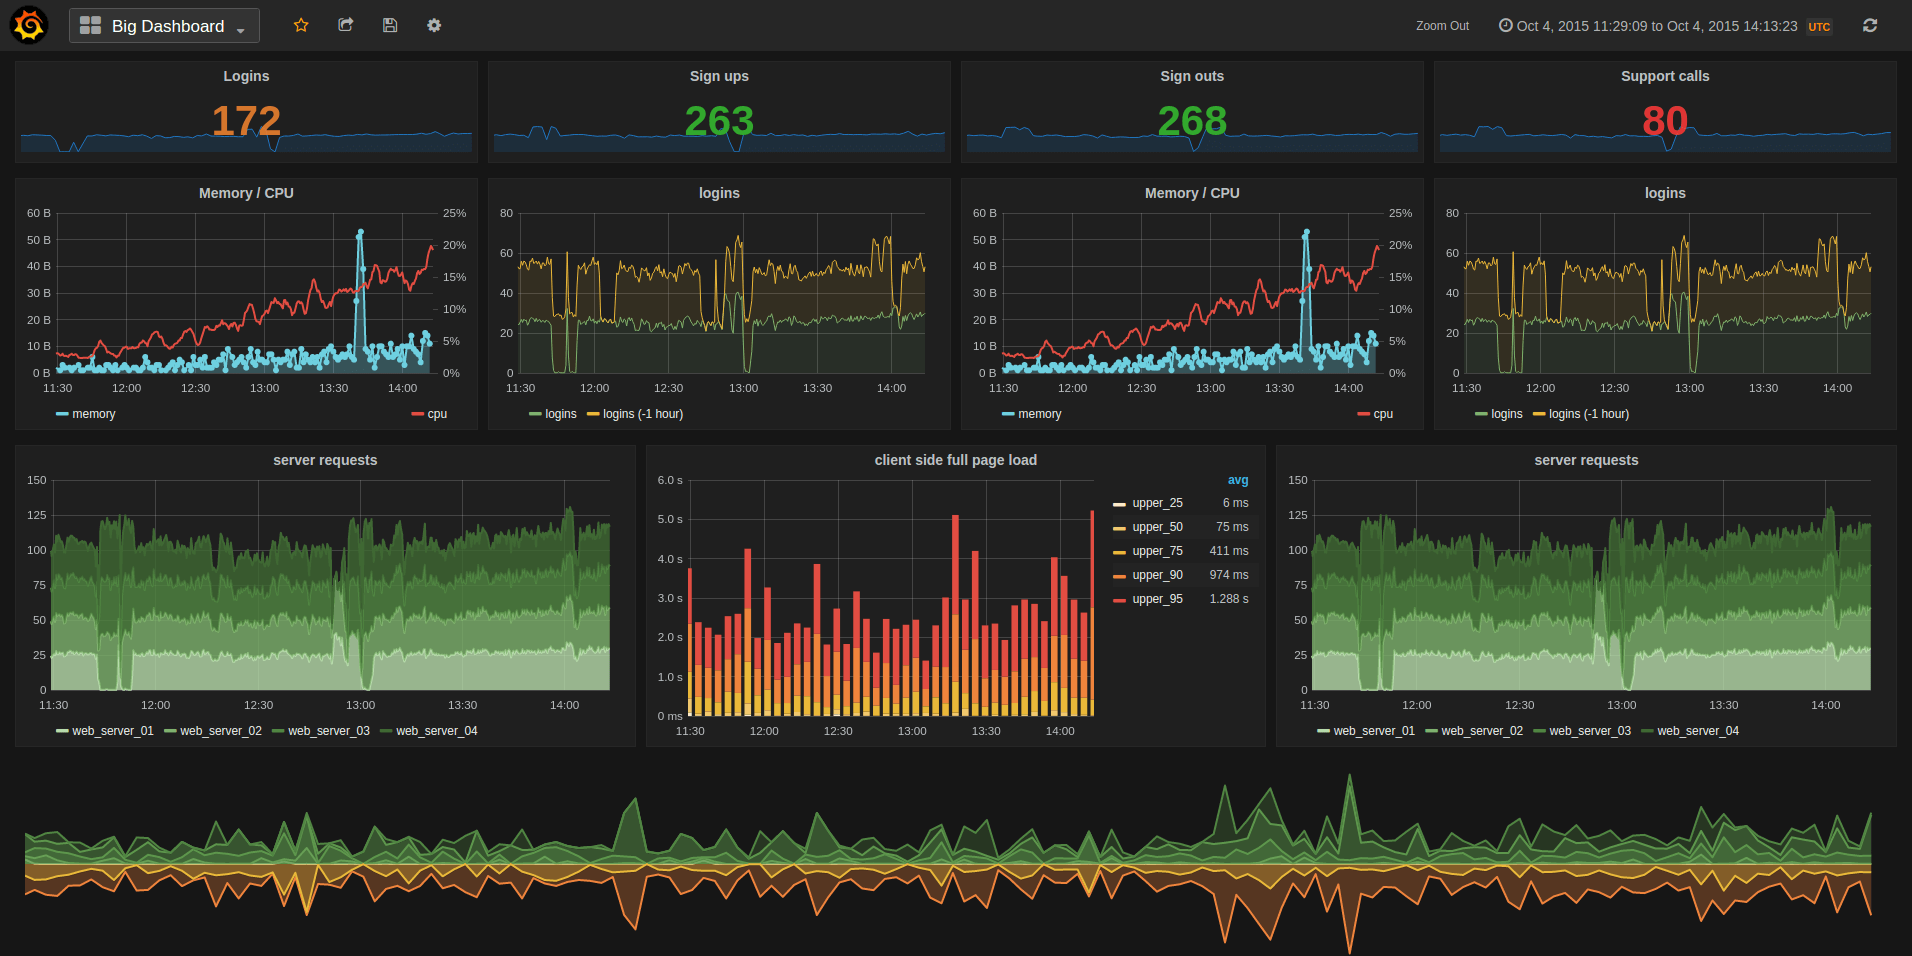
\includegraphics{source/figures/dashboard.png}
\caption{Dashboard de ejemplo de Grafana \label{dashboard}}
\end{figure}

\subsection{Monitorización}\label{monitorizaciuxf3n}

La monitorización es una parte importante para controlar la estabilidad
del sistema, sin unas herramientas adecuadas no podemos asegurar la
disponibilidad y el buen funcionamiento de nuestro software, para ello
existen diferentes herramientas, como la anteriormente mencionada
\emph{Grafana} y a nivel de procesos \emph{monit}, monit nos asegura que
nuestros servicios estarán siempre levantados, si hay alguna caída, la
herramienta los volverá a levantar.

\subsection{Alertas}\label{alertas}

En caso de caída de servicio necesitamos tener un sistema de alertas que
nos comunique el fallo correspondiente, para ello se utilizará además de
\emph{monit}, \emph{Sensu}, que es un sistema configurable de checks
para nuestros servicios, \emph{Sensu} es a su vez compatible con
sistemas de alerta a equipos de operaciones, como por ejemplo
\emph{OpsGenie}.

(Anthony Molinaro 2005)

(Abraham Silberschatz 1986)

(Erich Gamma 1994)

(Martin Fowler 2002)

(Martin Fowler 1997)

(Dennis Hutten 2016)

(Kent Beck 2003)

(Roy Greenfeld 2016)

(Mark Lutz 2013)

(Mark Lutz 2014)

(Steve McConnell 2004)

(Hunt 1999)

(J.W. Percival 2014)

(Python 2017)

(Django 2017)

\chapter{Implementación}\label{implementaciuxf3n-1}

Llegada la etapa de implementación, hay que transformar a código lo
analizado y diseñado en etapas anteriores. La idea original era hacer
una aplicación web, esta aplicación estaría separada en dos subsistemas,
uno de administración y otro de integración con aplicaciones.

\section{Subsistema de
administración}\label{subsistema-de-administraciuxf3n}

Este subsistema consiste en una aplicación web con diferentes paneles
para gestionar cada una de las partes del sistema, usuarios, empresas,
etc.

A este subsistema tendrán acceso los administradores de la empresa
principal con licencia del software, cada usuario tendrá visibilidad
limitada según sus permisos. Empresas externas clientes de la empresa
licenciada podrán tener acceso pero con visibilidad muy limitada, solo
para gestionar los usuarios propios y el acceso a las aplicaciones que
tenga contratadas.

\subsection{Lenguajes}\label{lenguajes}

Para esta sección se ha utilizado \emph{Python} como lenguaje principal,
usando \emph{Django} como framework de desarrollo web. La razón por la
que se eligen \emph{Python} y \emph{Django} es por la actual experiencia
del autor del proyecto en estos lenguajes, además de existir una
comunidad bastante grande alrededor de ellos, con una documentación
amplia disponible.

\emph{Python} es un lenguaje fácil de aprender y con parecido al
lenguaje natural, por lo que facilita la labor a la hora de hacer un
proyecto de estas características, \emph{Django} además provee de
diferentes herramientas para abstraer el desarrollo de una aplicación
web e implementar solo la lógica de negocio.

\emph{Django} sigue una variación del patrón MVC, en el cual separa la
capa de modelo de datos del resto, en esta capa está la lógica del
dominio del negocio, aunque se puede separar en más subniveles. En lugar
del clásico controlador, \emph{Django} usa el concepto de Vista, que son
funciones que reciben la petición del servidor y devuelven una respuesta
acorde utilizando la lógica de los modelos. El equivalente a la vista
del MVC sería en este caso el sistema de plantillas, plantillas que dado
el caso la View de \emph{Django} renderiza con los datos necesarios.

Para la interfaz se ha aprovechado la librería \emph{django-admin} que
autogenera formularios para los modelos implementados, además sobre esta
se utiliza una capa llamada \emph{django-suit} para mejorar el resultado
de la interfaz que se mostrará al usuario, esto ahorra trabajo de
maquetación y diseño, trabajos que escapan al alcance de este proyecto.

\section{Subsistema de integración}\label{subsistema-de-integraciuxf3n}

Este subsistema consiste en una API REST para que las aplicaciones
puedan interactuar con el sistema central, este subsistema pone a
disposición de la aplicación tokens de acceso con los cuales puede
acceder a la API y realizar diferentes labores, además de identificar al
usuario.

\subsection{Lenguajes}\label{lenguajes-1}

Para este subsistema se ha utilizado también \emph{Python} y
\emph{Django} pero con el añadido de usar \emph{django-rest-framework}
como capa por encima de \emph{Django}.

Este framework nos proporciona varias herramientas para construir una
API REST con \emph{Django}, como son los serializadores y las vistas
genéricas.

\subsection{Herramientas utilizadas}\label{herramientas-utilizadas}

Para el desarrollo del proyecto se hace necesario el uso de una serie de
herramientas, como editores de código, sistemas de control de versiones,
etc.

A continuación se detallarán todas las herramientas usadas en este
proyecto.

La herramienta principal que se ha utilizado ha sido un IDE, en este
caso \emph{PyCharm}. \emph{PyCharm} es un entorno escrito en Java y
pensado en un principio para desarrollar proyectos Python, es una
evolución de \emph{IntellijIdea}, el cual es una herramienta para
desarrollar \emph{Java}, pero conforme ha avanzado el tiempo se ha ido
ampliando a más lenguajes, como por ejemplo Python. La integración con
este último es perfecta, proporcionando útiles herramientas como el
autocompletado.

Para la detección de errores se hace casi obligado el uso de un
debugger, en este caso hemos usado el debugger integrado de PyCharm,
permitiendo utilizar puntos de ruptura en el código para comprobar el
estado del sistema en un momento dado.

Para el despliegue de la aplicación se ha utilizado un entorno compuesto
por un servidor Nginx, base de datos MySQL y el intérprete de
\emph{Python}, todo ello sobre un sistema GNU/Linux.

Otra herramienta utilizada que facilita el trabajo enormemente ha sido
Git. Git es un sistema de control de versiones que facilita el
desarrollo colaborativo y el mantenimiento de un software, versionando
todos los cambios que se vayan produciendo en el código. Esto permite
que si queremos volver a una versión anterior del sistema podamos
hacerlo sin problema alguno, además de la creación de ramas de
desarrollo, pudiendo fusionar ramas sin problema alguno.

\section{Detalles de implementación de la arquitectura del
sistema}\label{detalles-de-implementaciuxf3n-de-la-arquitectura-del-sistema}

\subsection{Capa modelo}\label{capa-modelo}

Como hemos dicho se ha utilizado \emph{Django} como framework de
desarrollo, \emph{Django} trae integrado un ORM que abstrae el acceso a
base de datos, funcionando de forma agnóstica con cualquier SGBD. Para
construir un modelo definimos sus atributos de clase, además de sus
relacione, utilizando los modelos que nos proporciona \emph{Django}.
\emph{Django} a su vez, utilizando el comando \texttt{make\ migrations}
generará las migraciones correspondientes que una vez ejecutadas con
\texttt{migrate} se aplicarán en la base de datos y crearán las tablas
necesarias.

Un ejemplo de modelo es el siguiente:

\begin{Shaded}
\begin{Highlighting}[]

\KeywordTok{class}\NormalTok{ Account(models.Model):}
\NormalTok{    objects }\OperatorTok{=}\NormalTok{ AccountManager()}

\NormalTok{    EMAIL_FIELD_MAX_LENGTH }\OperatorTok{=} \DecValTok{255}

    \BuiltInTok{id} \OperatorTok{=}\NormalTok{ models.AutoField(primary_key}\OperatorTok{=}\VariableTok{True}\NormalTok{,}
\NormalTok{                          help_text}\OperatorTok{=}\StringTok{"the account id, e.g. 1234"}\NormalTok{)}
\NormalTok{    uid }\OperatorTok{=}\NormalTok{ UUIDField(default}\OperatorTok{=}\NormalTok{get_uuid,}
\NormalTok{                    help_text}\OperatorTok{=}\StringTok{"A unique uuid string"}\NormalTok{)}
\NormalTok{    enabled }\OperatorTok{=}\NormalTok{ models.BooleanField(default}\OperatorTok{=}\VariableTok{True}\NormalTok{,}
\NormalTok{                                  help_text}\OperatorTok{=}\NormalTok{(}\StringTok{"A flag that indicates if the account is enabled or "}
                                             \StringTok{"not. A disabled account cannot log in the system and"}
                                             \StringTok{"will not receive notifications."}\NormalTok{))}
\NormalTok{    email }\OperatorTok{=}\NormalTok{ models.EmailField(max_length}\OperatorTok{=}\NormalTok{EMAIL_FIELD_MAX_LENGTH,}
\NormalTok{                              help_text}\OperatorTok{=}\StringTok{"Account email, e.g. example@gmail.com"}\NormalTok{)}
\NormalTok{    password }\OperatorTok{=}\NormalTok{ models.CharField(max_length}\OperatorTok{=}\DecValTok{56}\NormalTok{,}
\NormalTok{                                help_text}\OperatorTok{=}\StringTok{"The account holder's password."}\NormalTok{)}
\NormalTok{    name }\OperatorTok{=}\NormalTok{ models.CharField(max_length}\OperatorTok{=}\DecValTok{40}\NormalTok{,}
\NormalTok{                            help_text}\OperatorTok{=}\StringTok{"The account holder's name."}\NormalTok{)}
\end{Highlighting}
\end{Shaded}

Una capa intermedia de los modelos es la capa de Model Managers, esta
capa permite abstraer diferentes consultas a la base de datos para no
repetirlas cada vez.

Un ejemplo sería el siguiente:

\begin{Shaded}
\begin{Highlighting}[]
\KeywordTok{class}\NormalTok{ AccountManager(models.Manager):}
    \AttributeTok{@transaction.atomic}
    \KeywordTok{def}\NormalTok{ create(}\VariableTok{self}\NormalTok{, }\OperatorTok{**}\NormalTok{kwargs):}
\NormalTok{        account }\OperatorTok{=} \BuiltInTok{super}\NormalTok{(AccountManager, }\VariableTok{self}\NormalTok{).create(}\OperatorTok{**}\NormalTok{kwargs)}
\NormalTok{        account.groups.add(}\VariableTok{self}\NormalTok{.default_group)}
        \ControlFlowTok{return}\NormalTok{ account}

    \AttributeTok{@cached_property}
    \KeywordTok{def}\NormalTok{ default_group(}\VariableTok{self}\NormalTok{):}
        \ControlFlowTok{return}\NormalTok{ Group.objects.get_by_natural_key(}\StringTok{'default'}\NormalTok{)}

    \KeywordTok{def}\NormalTok{ get_by_id_or_uid(}\VariableTok{self}\NormalTok{, uid):}
        \ControlFlowTok{if} \BuiltInTok{isinstance}\NormalTok{(uid, }\BuiltInTok{int}\NormalTok{) }\KeywordTok{or}\NormalTok{ uid.isdigit():}
\NormalTok{            params }\OperatorTok{=}\NormalTok{ \{}\StringTok{'pk'}\NormalTok{: uid\}}
        \ControlFlowTok{elif} \BuiltInTok{len}\NormalTok{(uid) }\OperatorTok{==} \DecValTok{32}\NormalTok{:}
\NormalTok{            params }\OperatorTok{=}\NormalTok{ \{}\StringTok{'uid'}\NormalTok{: uid\}}
        \ControlFlowTok{else}\NormalTok{:}
            \ImportTok{from}\NormalTok{ api.models }\ImportTok{import}\NormalTok{ Account}
            \ControlFlowTok{raise}\NormalTok{ Account.DoesNotExist()}

        \ControlFlowTok{return} \VariableTok{self}\NormalTok{.get(}\OperatorTok{**}\NormalTok{params)}
\end{Highlighting}
\end{Shaded}

En cuanto a las migraciones, son sentencias que permiten versionar los
cambios en la base de datos, un ejemplo sería el siguiente:

\begin{Shaded}
\begin{Highlighting}[]

\KeywordTok{class}\NormalTok{ Migration(migrations.Migration):}

\NormalTok{    dependencies }\OperatorTok{=}\NormalTok{ [}
\NormalTok{    ]}

\NormalTok{    operations }\OperatorTok{=}\NormalTok{ [}
\NormalTok{        migrations.CreateModel(}
\NormalTok{            name}\OperatorTok{=}\StringTok{'Account'}\NormalTok{,}
\NormalTok{            fields}\OperatorTok{=}\NormalTok{[}
\NormalTok{                (}\StringTok{'id'}\NormalTok{, models.AutoField(serialize}\OperatorTok{=}\VariableTok{False}\NormalTok{, primary_key}\OperatorTok{=}\VariableTok{True}\NormalTok{, db_column}\OperatorTok{=}\NormalTok{b}\StringTok{'ac_id'}\NormalTok{)),}
\NormalTok{                (}\StringTok{'enabled'}\NormalTok{, models.BooleanField(default}\OperatorTok{=}\VariableTok{True}\NormalTok{, db_column}\OperatorTok{=}\NormalTok{b}\StringTok{'ac_enabled'}\NormalTok{)),}
\NormalTok{                (}\StringTok{'email'}\NormalTok{, models.EmailField(max_length}\OperatorTok{=}\DecValTok{255}\NormalTok{, db_column}\OperatorTok{=}\NormalTok{b}\StringTok{'ac_email'}\NormalTok{)),}
\NormalTok{                (}\StringTok{'password'}\NormalTok{, models.CharField(max_length}\OperatorTok{=}\DecValTok{56}\NormalTok{, db_column}\OperatorTok{=}\NormalTok{b}\StringTok{'ac_password'}\NormalTok{)),}
\NormalTok{                (}\StringTok{'name'}\NormalTok{, models.CharField(max_length}\OperatorTok{=}\DecValTok{40}\NormalTok{, db_column}\OperatorTok{=}\NormalTok{b}\StringTok{'ac_name'}\NormalTok{)),}
\NormalTok{                (}\StringTok{'surname'}\NormalTok{, models.CharField(default}\OperatorTok{=}\NormalTok{b}\StringTok{''}\NormalTok{, max_length}\OperatorTok{=}\DecValTok{40}\NormalTok{, db_column}\OperatorTok{=}\NormalTok{b}\StringTok{'ac_surname'}\NormalTok{, blank}\OperatorTok{=}\VariableTok{True}\NormalTok{)),}
\NormalTok{            ],}
\NormalTok{            options}\OperatorTok{=}\NormalTok{\{}
                \StringTok{'db_table'}\NormalTok{: }\StringTok{'Account'}\NormalTok{,}
\NormalTok{            \},}
\NormalTok{        ),}
\end{Highlighting}
\end{Shaded}

\subsection{Capa View (Controlador)}\label{capa-view-controlador}

La capa controlador es la que se encarga de recibir las peticiones de la
api y devolver una respuesta adecuada, es la capa de interfaz al
exterior por lo que es bastante importante.

El controlador se compone de un Router y las Vistas, el Router se
encarga de parsear las urls y pasar la petición a la vista
correspondiente, un ejemplo de router sería el siguiente:

\begin{Shaded}
\begin{Highlighting}[]
\NormalTok{urlpatterns }\OperatorTok{=}\NormalTok{ [}
\NormalTok{    url(}
\NormalTok{        regex}\OperatorTok{=}\VerbatimStringTok{r'^$'}\NormalTok{,}
\NormalTok{        view}\OperatorTok{=}\NormalTok{views.UserListView.as_view(),}
\NormalTok{        name}\OperatorTok{=}\StringTok{'list'}
\NormalTok{    ),}
\NormalTok{    url(}
\NormalTok{        regex}\OperatorTok{=}\VerbatimStringTok{r'^~redirect/$'}\NormalTok{,}
\NormalTok{        view}\OperatorTok{=}\NormalTok{views.UserRedirectView.as_view(),}
\NormalTok{        name}\OperatorTok{=}\StringTok{'redirect'}
\NormalTok{    ),}
\NormalTok{    url(}
\NormalTok{        regex}\OperatorTok{=}\VerbatimStringTok{r'^companies/(?P<slug>[\textbackslash{}w.@+-]+)/users/(?P<username>[\textbackslash{}w.@+-]+)/$'}\NormalTok{,}
\NormalTok{        view}\OperatorTok{=}\NormalTok{views.UserDetailView.as_view(),}
\NormalTok{        name}\OperatorTok{=}\StringTok{'detail'}
\NormalTok{    ),}
\NormalTok{    url(}
\NormalTok{        regex}\OperatorTok{=}\VerbatimStringTok{r'^~update/$'}\NormalTok{,}
\NormalTok{        view}\OperatorTok{=}\NormalTok{views.UserUpdateView.as_view(),}
\NormalTok{        name}\OperatorTok{=}\StringTok{'update'}
\NormalTok{    ),}
\NormalTok{]}
\end{Highlighting}
\end{Shaded}

Las vistas genéricas de \emph{django-rest-framework} se componen de
varios atributos para configurarlas, permitiendo generar una respuesta
sin escribir apenas código, un ejemplo sería el siguiente:

\begin{Shaded}
\begin{Highlighting}[]

\KeywordTok{class}\NormalTok{ AccountDetailView(generics.RetrieveUpdateDestroyAPIView):}
\NormalTok{    queryset }\OperatorTok{=}\NormalTok{ Account.objects.}\BuiltInTok{all}\NormalTok{()}
\NormalTok{    serializer_class }\OperatorTok{=}\NormalTok{ AccountSerializer}
\NormalTok{    permission_classes }\OperatorTok{=}\NormalTok{ (UserCanManagePermission,)}
\NormalTok{    lookup_field }\OperatorTok{=} \StringTok{'id'}
\NormalTok{    lookup_url_kwarg }\OperatorTok{=} \StringTok{'account_id'}
\end{Highlighting}
\end{Shaded}

La vista del ejemplo genera acciones para el GET en detalle, para el PUT
y para el DELETE, utilizando el queryset configurado.

\subsection{Capa Templates (Vista)}\label{capa-templates-vista}

Para esta capa hemos utilizado \emph{django-admin} con la capa de
\emph{django-suit}, las vistas se configuran mediante código Python y en
parte se autogeneran a partir de los modelos.

Ejemplo:

\begin{Shaded}
\begin{Highlighting}[]
\KeywordTok{class}\NormalTok{ AccountAdmin(DjangoObjectActions, admin.ModelAdmin):}
\NormalTok{    model }\OperatorTok{=}\NormalTok{ Account}
\NormalTok{    list_display }\OperatorTok{=}\NormalTok{ (}\StringTok{'id'}\NormalTok{, }\StringTok{'name'}\NormalTok{, }\StringTok{'enabled'}\NormalTok{)}
\NormalTok{    list_filter }\OperatorTok{=}\NormalTok{ [}\StringTok{'enabled'}\NormalTok{]}
\NormalTok{    search_fields }\OperatorTok{=}\NormalTok{ [}\StringTok{'name'}\NormalTok{]}

\NormalTok{    readonly_fields }\OperatorTok{=}\NormalTok{ []}

    \KeywordTok{def}\NormalTok{ get_readonly_fields(}\VariableTok{self}\NormalTok{, request, obj}\OperatorTok{=}\VariableTok{None}\NormalTok{):}
        \ControlFlowTok{return}\NormalTok{ [f.name }\ControlFlowTok{for}\NormalTok{ f }\KeywordTok{in} \VariableTok{self}\NormalTok{.model._meta.fields]}
\end{Highlighting}
\end{Shaded}

\chapter{Seguridad}\label{seguridad}

Cuando comercializamos una aplicación que contendrá datos sensibles de
usuarios y empresas como esta un aspecto importante es asegurar que
todos estos datos son accedidos solo por la gente que debe, además de
asegurar la persistencia e integridad de estos datos.

\section{Seguridad para el software}\label{seguridad-para-el-software}

Es importante poder tracear de que forma se ha accedido al sistema y
quién ha modificado cada cosa. Para ello es importante mantener un
registro de auditoría del sistema.

\subsection{Subsistema de
administración}\label{subsistema-de-administraciuxf3n-1}

Para el subsistema de administración se mantiene un log de eventos en
forma de tabla en la base de datos, este log indica cada acción
realizada, sobre que tabla y qué usuario, además se almacenan también
los intentos de acceso al sistema de administración.

\subsection{Subsistema de
integración}\label{subsistema-de-integraciuxf3n-1}

Al igual que en el otro subsistema, en este caso se hace necesario saber
qué aplicación está accediendo y en nombre de quién, para ello en la
misma tabla anterior añadimos un campo application\_id, para saber desde
qué aplicación se está realizando la modificación, siendo nulo en caso
de haberse realizado directamente desde el panel de administración.

\subsection{Logs}\label{logs}

Además de los datos anteriores, es necesario guardar logs de aplicación
en el servidor de logs correspondiente, para ello utilizamos la
herramienta \emph{syslog-ng} para redirigir los logs generados por la
aplicación al servidor correspondiente. La aplicación debe generar logs
útiles de todas las acciones que se realicen, de forma que sean
trazables.

\section{Seguridad de los datos}\label{seguridad-de-los-datos}

Al ser una aplicación multi-tenant los datos no deben ser accesibles de
un cliente a otro, ya que en principio no estarían físicamente
separados, la forma de hacerlo será por software, en forma de esquemas
diferentes de base de datos, asegurando así que no serán accedidos de un
tenant a otro.

\subsection{Copias de seguridad}\label{copias-de-seguridad}

Al no ser datos extremadamente críticos se decide hacer una copia de
seguridad al día, esta copia está gestionada por AWS, de forma que no
tenemos que preocuparnos mucho más que de configurarla.

\subsection{Mecanismos de integridad}\label{mecanismos-de-integridad}

La base de datos ayudada por el ORM mantiene en todo momento integridad
referencial, al ser una base de datos SQL con sus relaciones definidas.

\section{Seguridad para el usuario}\label{seguridad-para-el-usuario}

También se debe asegurar que cada usuario y cada aplicación solo accede
a los datos que debe, para ello se configuran permisos para cada usuario
y luego se añade la capa de OAuth, para la cual solo se otorgan permisos
limitados por token. A continuación se explicará el protocolo OAuth 2.0
en detalle.

\subsection{OAuth}\label{oauth}

OAuth 2.0 es el protocolo estándar de la industria para autorización.
OAuth 2.0 se enfoca en la simplicidad para proveer flujos de
autorizaciones para aplicaciones, ya sean de tipo web, escritorio,
móvil, etc. OAuth es una especificación desarrollada en el marco de la
IETF.

\subsubsection{Flujos de OAuth}\label{flujos-de-oauth}

OAuth dispone de varios flujos de funcionamiento, en función de si la
aplicación es pública o privada. A continuación se explicarán todos los
flujos disponibles.

\paragraph{Flujo de autorización en 3
pasos}\label{flujo-de-autorizaciuxf3n-en-3-pasos}

Este flujo está pensado para aplicaciones públicas de terceros, en las
cuales no queremos que la aplicación tenga acceso a las credenciales de
usuario, para ello en primer lugar se envía al usuario al servidor de
autorización, mostrando una interfaz para introducir sus credenciales,
estas credenciales son introducidas directamente en el servidor, por lo
que la aplicación no tiene acceso a ellas.

Una vez validadas el servidor devuelve un código temporal de
autorización a la aplicación, que debe disponer de un servidor con una
url para recoger este código.

Una vez obtenido el código este debe ser intercambiado por un token de
acceso definitivo, para ello con el código y las credenciales de
aplicación, ésta realiza una petición al servidor de autorización para
intercambiar el código por un token, el servidor devuelve el token y el
código deja de ser válido.

\paragraph{Flujo de autorización en 2
pasos}\label{flujo-de-autorizaciuxf3n-en-2-pasos}

Este flujo existe para aplicaciones públicas confiables, en principio
aplicaciones desarrolladas por el mismo proveedor de autorización pero
que funcionan de forma pública, tipo aplicaciones móvil, etc. En estas
aplicaciones conocemos que no almacenarán las credenciales del usuario
por lo que son confiables.

En primer lugar la aplicación realiza una petición al servidor con las
credenciales de aplicación y de usuario, el servidor responde
directamente con el token de acceso y la aplicación ya puede empezar a
funcionar.

\paragraph{Flujo de autorización para
aplicaciones}\label{flujo-de-autorizaciuxf3n-para-aplicaciones}

Este flujo existe para aplicaciones privadas desarrolladas por el
proveedor de autorización, que son totalmente confiables, estas
aplicaciones utilizan solamente sus credenciales de aplicación, sin
necesitar las de usuario, y en principio tendrían más privilegios que
las normales, ya que no están disponibles de forma pública.

En primer lugar la aplicación realiza una petición al servidor enviando
sus credenciales, el servidor responde con un token de acceso.

\subsection{Permisos}\label{permisos}

Cada usuario tiene unos permisos definidos con lo que puede ver en el
sistema, además de esto se pueden configurar permisos personalizados por
aplicación que serán otorgados luego al usuario.

\subsection{Scopes}\label{scopes}

Los scopes son permisos que la aplicación obtiene sobre un usuario para
actuar en su nombre.

\section{Seguridad del hardware}\label{seguridad-del-hardware}

Esta capa a pesar de ser importante está gestionada por AWS, al haber
configurado los sistemas de forma que sean fácilmente replicables no
tenemos que preocuparnos por este aspecto.

\chapter{Pruebas}\label{pruebas-1}

Todo software que se precie requiere de una suite de pruebas que asegure
la calidad del software. En muchas ocasiones se tiende a usar una
metodología de desarrollo TDD (Test Driven Development), en la cual se
escriben primero los tests para que fallen y a continuación se va
implementando el software para hacer pasar esos tests fallidos. Esta
metodología de desarrollo facilita pensar primero en la solución y el
objetivo final a implementar, además de desarrollar una solución rápida,
además permite tener una base sobre la que refactorizar luego el código
de forma segura. TDD es una metodología útil, pero no debería de ser el
único marco de desarrollo que utilizáramos para asegurar la calidad del
software. Para ello se ha de hacer primero un plan de pruebas que
asegure la calidad de todo el proceso de creación del mismo, desde el
análisis hasta la implementación final.

Este documento pretende generar un plan de pruebas acorde a la
documentación generada en las secciones anteriores, revisándo de esta
forma los pasos anteriores y actualizando lo que no tuviera sentido o lo
que faltara por contemplar. Para ello distinguiremos entre las
diferentes categorías de pruebas, desde las \emph{unitarias} hasta las
de \emph{aceptación}, entrando más en detalle en las últimas, ya que son
las que asegurarán la calidad de los diferentes casos de uso. Estas
pruebas deberán llevarse a cabo de forma automática, y lanzarse
previamente a una release de software para asegurar que esta release
cumple con los requisitos de aceptación previamente elicitados. El
resultado de este informe debería ser revisado por el equipo de calidad
(Quality Assurance) de forma que nos aseguremos que los requisitos se
cumplen. El documento de aceptación debería ser generado conjuntamente
también con este equipo, de forma que su trabajo pase por todas las
etapas del ciclo de vida del software, no solo al final como se hacía
clásicamente.

\section{Test Driven Development}\label{test-driven-development}

Test-driven development es un proceso de desarrollo de software ideado
por Kent Beck que basa el desarrollo en la repetición de un ciclo corto
del mismo. De esta forma los requisitos se transforman en casos de
prueba muy específicos, estos casos se implementan y el software se va
mejorando para pasar estos tests solamente, sin añadir ningún tipo de
lógica más. Este sistema se contrapone al clásico que permitía añadir
código sin pruebas para que estas fueran añadidas a posteriori.

Kent Beck afirmó que TDD incentiva diseños simples e inspira confianza
en el software. Esta confianza crece ya que una vez implementado un caso
de uso con unos tests que nos aseguran que funciona, podemos
refactorizar sin miedo alguno de romper nada, ya que en el momento que
algo se rompa los tests nos lo indicarán.

Esta metodología nace de los conceptos de programación extrema,
metodología que nació en 1999, adquiriendo en los últimos años entidad
propia.

\section{Pruebas unitarias}\label{pruebas-unitarias}

Una parte importante del desarrollo de software son las pruebas
unitarias, también conocidas como pruebas de caja negra, este tipo de
pruebas prueban piezas de software de forma aislada, asegurando que con
una entrada concreta recibimos la salida que queremos, en nuestro
proyecto hemos querido limitar este tipo de pruebas, ya que a pesar de
ser importantes, no aseguran el funcionamiento de forma integrada de
todas las piezas, consideramos más importantes los tests de aceptación
que prueban el software de punto a punto.

Aun así para piezas con cierta complejidad se hace casi obligatorio
escribir este tipo de tests automáticos, estos tests pueden actuar
además como documentación de esas piezas de software complejas, de forma
que otros desarrolladores comprendan mejor su funcionamiento.

\section{Pruebas de aceptación}\label{pruebas-de-aceptaciuxf3n}

La prueba de aceptación es la última de las pruebas que debe atravesar
una aplicación en un plan de QA, es la que prueba el software desde el
punto de vista del usuario y prueba la integración de todas las piezas
del sistema. Si la especificación es completa y las pruebas están
pensadas, éstas deberían ser suficientes para cubrir casi todos los
casos en los que un usuario dará uso al software.

Normalmente para las pruebas de aceptación se trabaja sobre historias de
usuario, que son casos de uso definidos desde el punto de vista del
usuario, para desarrollar este plan de pruebas partiremos de los casos
de uso elicitados en el capítulo de análisis.

\subsection{Caso de uso Añadir
usuario}\label{caso-de-uso-auxf1adir-usuario-2}

\begin{itemize}
\tightlist
\item
  Historia de usuario: \emph{Yo como usuario administrador de mi empresa
  X, quiero poder añadir un usuario en el sistema dentro de mi empresa.}
\item
  Pruebas de aceptación:

  \begin{itemize}
  \tightlist
  \item
    Si el usuario identificado no tiene rol de administrador se
    devolverá un error en el que se indique que no hay permisos.
  \item
    Si el usuario envía algún dato incorrecto se devolverá un error
    indicando de forma detallada el error.
  \item
    Si el usuario envía un email ya existente se devolverá un error
    indicándolo.
  \item
    Una vez finalizado el proceso el usuario aparece en la lista de
    usuarios inactivos de la empresa.
  \item
    Una vez finalizado el proceso el usuario recibe un email para
    terminar el registro.
  \end{itemize}
\end{itemize}

\subsection{Caso de uso Terminar configuración de
usuario}\label{caso-de-uso-terminar-configuraciuxf3n-de-usuario-1}

\begin{itemize}
\tightlist
\item
  Historia de usuario: \emph{Yo como usuario recién reigstrado quiero
  terminar el proceso de configuración para activar mi usuario}
\item
  Pruebas de aceptación:

  \begin{itemize}
  \tightlist
  \item
    Una vez finalizado el proceso el usuario aparece en el listado de
    usuarios activos de la empresa.
  \item
    Si alguno de los datos enviados es incorrectos el sistema debe
    indicar el error de forma detallada.
  \end{itemize}
\end{itemize}

\subsection{Caso de uso Editar
usuario}\label{caso-de-uso-editar-usuario-2}

\begin{itemize}
\tightlist
\item
  Historia de usuario: \emph{Yo como usuario X administrador de mi
  empresa, quiero poder editar un usuario Y diferente de mi en el
  sistema dentro de mi empresa.}
\item
  Pruebas de aceptación:

  \begin{itemize}
  \tightlist
  \item
    Si el usuario Y pertenece a una empresa diferente se devolverá un
    error en el que se indique que no hay permisos o que el usuario no
    existe dentro de la empresa.
  \item
    Si el usuario identificado no tiene rol de administrador se
    devolverá un error en el que se indique que no hay permisos.
  \item
    Si el usuario envía algún dato incorrecto se devolverá un error
    indicando de forma detallada el error.
  \item
    Si el usuario envía un email ya existente se devolverá un error
    indicándolo.
  \item
    Una vez finalizado el proceso, en la vista del usuario actualizado
    aparecerán los datos modificados actualizados.
  \end{itemize}
\item
  Historia de usuario: \emph{Yo como usuario de mi empresa X, quiero
  poder editar mi contraseña en el sistema}
\item
  Pruebas de aceptación:

  \begin{itemize}
  \tightlist
  \item
    Si la contraseña no tiene el nivel de seguridad mínimo se devolverá
    un error indicándolo.
  \item
    Una vez finalizado el proceso, la contraseña del usuario quedará
    actualizada y podrá crear tokens con la nueva contraseña, también
    sus tokens anteriores quedarán invalidados.
  \end{itemize}
\end{itemize}

\subsection{Caso de uso Ver usuario}\label{caso-de-uso-ver-usuario}

\begin{itemize}
\tightlist
\item
  Historia de usuario: \emph{Yo como usuario X administrador de mi
  empresa, quiero poder ver los datos de un usuario Y diferente de mi
  perteneciente a mi misma empresa.}
\item
  Pruebas de aceptación:

  \begin{itemize}
  \tightlist
  \item
    Si el usuario Y pertenece a una empresa diferente se devolverá un
    error en el que se indique que no hay permisos o que el usuario no
    existe dentro de la empresa.
  \item
    Si el usuario identificado no tiene rol de administrador se
    devolverá un error en el que se indique que no hay permisos.
  \item
    Si todo es correcto se devolverán los datos del usuario excluyendo
    su contraseña.
  \end{itemize}
\item
  Historia de usuario: \emph{Yo como usuario X, quiero poder ver mis
  datos.}
\item
  Pruebas de aceptación:

  \begin{itemize}
  \tightlist
  \item
    Si el usuario solicitado es diferente al identificado se devolverá
    un error en el que se indique que no hay permisos o que el usuario
    no existe dentro de la empresa.
  \item
    Si todo es correcto se devolverán los datos del usuario excluyendo
    su contraseña.
  \end{itemize}
\end{itemize}

\subsection{Caso de uso Borrar
usuario}\label{caso-de-uso-borrar-usuario-1}

\begin{itemize}
\tightlist
\item
  Historia de usuario: \emph{Yo como usuario X, administrador de mi
  empresa, quiero poder borrar un usuario Y diferente a mi.}
\item
  Pruebas de aceptación:

  \begin{itemize}
  \tightlist
  \item
    Si el usuario solicitado es X, no se permitirá continuar por
    seguridad, primero otro administrador deberá quitarle el privilegio
    de administrador y borrarle.
  \item
    Si el usuario identificado no tiene rol de administrador se
    devolverá un error en el que se indique que no hay permisos.
  \item
    Si el proceso es correcto el usuario Y dejará de aparecer en la
    lista de usuarios activos de la empresa.
  \end{itemize}
\end{itemize}

\subsection{Caso de uso Añadir
empresa}\label{caso-de-uso-auxf1adir-empresa-2}

\begin{itemize}
\tightlist
\item
  Historia de usuario: \emph{Yo como usuario administrador del sistema,
  quiero poder añadir una empresa en el sistema, de forma que aparezca
  en la lista de empresas disponibles.}
\item
  Pruebas de aceptación:

  \begin{itemize}
  \tightlist
  \item
    Si el usuario identificado no tiene rol de administrador se
    devolverá un error en el que se indique que no hay permisos.
  \item
    Si el usuario envía algún dato incorrecto se devolverá un error
    indicando de forma detallada el error.
  \item
    Si el usuario envía un nombre o código ya existente se devolverá un
    error indicándolo.
  \item
    Una vez finalizado el proceso la empresa aparecerá en la lista de
    empresas activas.
  \end{itemize}
\end{itemize}

\subsection{Caso de uso Editar
empresa}\label{caso-de-uso-editar-empresa-2}

\begin{itemize}
\tightlist
\item
  Historia de usuario: \emph{Yo como usuario administrador del sistema,
  quiero poder editar una empresa de las disponibles en el sistema, de
  forma que los datos queden actualizados.}
\item
  Pruebas de aceptación:

  \begin{itemize}
  \tightlist
  \item
    Si el usuario identificado no tiene rol de administrador se
    devolverá un error en el que se indique que no hay permisos.
  \item
    Si el usuario envía algún dato incorrecto se devolverá un error
    indicando de forma detallada el error.
  \item
    Si el usuario envía un nombre o código ya existente se devolverá un
    error indicándolo.
  \item
    Una vez finalizado el proceso los datos de la empresa quedarán
    actualizados.
  \end{itemize}
\end{itemize}

\subsection{Caso de uso Ver empresa}\label{caso-de-uso-ver-empresa}

\begin{itemize}
\tightlist
\item
  Historia de usuario: \emph{Yo como usuario administrador del sistema,
  quiero poder ver los datos de una empresa X.}
\item
  Pruebas de aceptación:

  \begin{itemize}
  \tightlist
  \item
    Si el usuario identificado no tiene rol de administrador se
    devolverá un error en el que se indique que no hay permisos.
  \item
    Una vez finalizado el proceso los datos de la empresa se devolverán
    al usuario.
  \end{itemize}
\item
  Historia de usuario: \emph{Yo como usuario administrador de la empresa
  X, quiero poder ver los datos de la empresa X.}
\item
  Pruebas de aceptación:

  \begin{itemize}
  \tightlist
  \item
    Si el usuario identificado pertenece a X pero no es administrador se
    devolverá un error indicando que no hay permisos.
  \item
    Si el usuario identificado no pertenece a X se devolverá un error
    indicando que X no existe.
  \item
    Una vez finalizado el proceso los datos de la empresa se devolverán
    al usuario.
  \end{itemize}
\end{itemize}

\subsection{Caso de uso Borrar
empresa}\label{caso-de-uso-borrar-empresa}

\begin{itemize}
\tightlist
\item
  Historia de usuario: \emph{Yo como usuario X, administrador del
  sistema quiero poder borrar una empresa Y y que esta desaparezca del
  listado de empresas disponibles.}
\item
  Pruebas de aceptación:

  \begin{itemize}
  \tightlist
  \item
    Si el usuario identificado no tiene rol de administrador se
    devolverá un error en el que se indique que no hay permisos.
  \item
    Si el proceso es correcto la empresa Y dejará de aparecer en la
    lista de empresas activas.
  \item
    Si el proceso es correcto todos los usuarios de la empresa Y dejarán
    de tener acceso y quedarán inhabilitados.
  \end{itemize}
\end{itemize}

\subsection{Caso de uso Registrar
aplicación}\label{caso-de-uso-registrar-aplicaciuxf3n-1}

\begin{itemize}
\tightlist
\item
  Historia de usuario: \emph{Yo, como usuario X, administrador del
  sistema, quiero poder registrar una aplicación en el sistema y que
  esta aparezca en el listado de aplicaciones disponibles.}
\item
  Pruebas de aceptación:

  \begin{itemize}
  \tightlist
  \item
    Si el usuario identificado no tiene rol de administrador se
    devolverá un error en el que se indique que no hay permisos.
  \item
    Una vez finalizado el proceso la aplicación aparecerá en la lista de
    aplicaciones activas.
  \item
    Si el usuario envía algún dato incorrecto se devolverá un error
    indicando de forma detallada el error.
  \item
    Si el usuario envía un nombre o código ya existente se devolverá un
    error indicándolo.
  \end{itemize}
\end{itemize}

\subsection{Caso de uso Editar
aplicación}\label{caso-de-uso-editar-aplicaciuxf3n-2}

\begin{itemize}
\tightlist
\item
  Historia de usuario: \emph{Yo, como usuario administrador del sistema,
  quiero poder editar una aplicación de las disponibles en el sistema,
  de forma que los datos queden actualizados.}
\item
  Pruebas de aceptación:

  \begin{itemize}
  \tightlist
  \item
    Si el usuario identificado no tiene rol de administrador se
    devolverá un error en el que se indique que no hay permisos.
  \item
    Si el usuario envía algún dato incorrecto se devolverá un error
    indicando de forma detallada el error.
  \item
    Si el usuario envía un nombre o código ya existente se devolverá un
    error indicándolo.
  \item
    Si el usuario selecciona una aplicación no existente, se devolverá
    un error indicándolo.
  \item
    Una vez finalizado el proceso los datos de la aplicación quedarán
    actualizados.
  \end{itemize}
\end{itemize}

\subsection{Caso de uso Ver
aplicación}\label{caso-de-uso-ver-aplicaciuxf3n}

\begin{itemize}
\tightlist
\item
  Historia de usuario: \emph{Yo, como usuario administrador del sistema,
  quiero poder ver los datos de una aplicación X.}
\item
  Pruebas de aceptación:

  \begin{itemize}
  \tightlist
  \item
    Si el usuario identificado no tiene rol de administrador se
    devolverá un error en el que se indique que no hay permisos.
  \item
    Una vez finalizado el proceso los datos de la aplicación se
    devolverán al usuario.
  \item
    Si el usuario selecciona una aplicación no existente, se devolverá
    un error indicándolo.
  \end{itemize}
\end{itemize}

\subsection{Caso de uso Borrar
aplicación}\label{caso-de-uso-borrar-aplicaciuxf3n-2}

\begin{itemize}
\tightlist
\item
  Historia de usuario: \emph{Yo como usuario X, administrador del
  sistema quiero poder borrar una empresa Y y que esta desaparezca del
  listado de empresas disponibles.}
\item
  Pruebas de aceptación:

  \begin{itemize}
  \tightlist
  \item
    Si el usuario identificado no tiene rol de administrador se
    devolverá un error en el que se indique que no hay permisos.
  \item
    Si el proceso es correcto la empresa Y dejará de aparecer en la
    lista de empresas activas.
  \item
    Si el proceso es correcto todos los usuarios de la empresa Y dejarán
    de tener acceso y quedarán inhabilitados.
  \end{itemize}
\end{itemize}

\subsection{Caso de uso Editar usuarios de empresa con acceso a
aplicación}\label{caso-de-uso-editar-usuarios-de-empresa-con-acceso-a-aplicaciuxf3n-1}

\begin{itemize}
\tightlist
\item
  Historia de usuario: \emph{Yo como usuario X, administrador de la
  empresa Y quiero poder dar acceso a un usuario U de mi empresa a una
  aplicación Z que tengo contratada.}
\item
  Pruebas de aceptación:

  \begin{itemize}
  \tightlist
  \item
    Si el usuario identificado no tiene rol de administrador se
    devolverá un error en el que se indique que no hay permisos.
  \item
    Si el usuario que quiero añadir no pertenece a mi empresa se
    mostrará un error.
  \item
    Si la aplicación Z no está contratada por mi empresa se mostrará un
    error.
  \item
    Una vez finalizado el proceso la aplicación Z podrá sacar un token
    en nombre del usuario U.
  \item
    Una vez finalizado el proceso el usuario U podrá usar la aplicación
    Z.
  \item
    Una vez finalizado el proceso el usuario U aparecerá en el listado
    de usuarios con acceso a Z.
  \end{itemize}
\end{itemize}

\subsection{Caso de uso Editar aplicaciones a las que tiene acceso una
empresa}\label{caso-de-uso-editar-aplicaciones-a-las-que-tiene-acceso-una-empresa}

\begin{itemize}
\tightlist
\item
  Historia de usuario: *Yo, como usuario X, administrador del sistema,
  quiero dar acceso a una empresa Y a una aplicación Z.
\item
  Pruebas de aceptación:

  \begin{itemize}
  \tightlist
  \item
    Si el usuario identificado no tiene rol de administrador se
    devolverá un error en el que se indique que no hay permisos.
  \item
    Si la aplicación no existe se mostrará un error.
  \item
    Si la empresa ya tiene acceso a la aplicación se mostrará un error.
  \item
    Una vez finalizado el proceso la aplicación aparecerá entre las
    disponibles para los administradores de la empresa Y.
  \end{itemize}
\end{itemize}

\subsection{Caso de uso Registrar aplicación
externa}\label{caso-de-uso-registrar-aplicaciuxf3n-externa-1}

\begin{itemize}
\tightlist
\item
  Historia de usuario: \emph{Yo, como usuario X, administrador del
  sistema, quiero poder registrar una aplicación externa en el sistema y
  que esta aparezca en el listado de aplicaciones disponibles.}
\item
  Pruebas de aceptación:

  \begin{itemize}
  \tightlist
  \item
    Si el usuario identificado no tiene rol de administrador se
    devolverá un error en el que se indique que no hay permisos.
  \item
    Una vez finalizado el proceso la aplicación aparecerá en la lista de
    aplicaciones activas.
  \item
    Si el usuario envía algún dato incorrecto se devolverá un error
    indicando de forma detallada el error.
  \item
    Si el usuario envía un nombre o código ya existente se devolverá un
    error indicándolo.
  \end{itemize}
\end{itemize}

\subsection{Caso de uso Obtener token de usuario desde
aplicación}\label{caso-de-uso-obtener-token-de-usuario-desde-aplicaciuxf3n}

\begin{itemize}
\tightlist
\item
  Historia de usuario: \emph{Yo, como usuario X, usuario de una empresa
  Y, quiero poder utilizar una aplicación registrada en el sistema a la
  que tengo acceso.}
\item
  Pruebas de aceptación:

  \begin{itemize}
  \tightlist
  \item
    Si el usuario no tiene acceso a la aplicación, el sistema devolverá
    un error que la aplicación deberá mostrar al usuario.
  \item
    Si el usuario tiene acceso a la aplicación, el sistema devolverá un
    token que la aplicación usará a partir de ese momento dando acceso
    al usuario.
  \end{itemize}
\end{itemize}

\chapter{Costes y monetización}\label{costes-y-monetizaciuxf3n}

La estimación de costes de desarrollo de un proyecto software es un
factor muy importante en el análisis de un proyecto, es parte
fundamental encontrar métricas para cuantificar el coste del mismo,
garantizando calidad y eficiencia. Por tanto podemos definir el análisis
de coste como el proceso de identificación de los recursos necesarios
para llevar a cabo el trabajo eficientemente.

\section{Estimación}\label{estimaciuxf3n}

Estimar el coste o tiempo que vamos a necesitar para desarrollar una
funcionalidad no es fácil. Hay diversos factores a tener en cuenta,
entre ellos el riesgo, la incertidumbre y la dificultad del trabajo en
sí. Cuanta más incertidumbre más complicado será dar una estimación con
precisión sobre el trabajo a realizar, ya que en muchas ocasiones se
comprende mejor el problema a medida que se avanza.

Para ello en este proyecto se ha decidido dar una estimación por días de
trabajo para cada funcionalidad, y ante la imposibilidad de dar una
estimación exacta se ha seguido la aproximación de dar un rango de
tiempo, siendo el rango de tiempo más amplio cuanta más incertidumbre
hay.

En cuanto a los costes, no tiene sentido hablar aquí de costes a
facturar cuando la aplicación está pensada para ser monetizada
ofreciéndola como servicio, no como un producto a medida. Pero de este
tema hablaremos en una sección posterior.

\subsection{Estimación por Caso de
Uso}\label{estimaciuxf3n-por-caso-de-uso}

En el caso de este proyecto se han decidido dar estimaciones por caso de
uso, ya que es la unidad más pequeña que tenemos para trabajar en el
software. Por tanto a continuación se darán estimaciones por caso de uso
en valor de días/persona de trabajo.

\begin{itemize}
\tightlist
\item
  Caso de uso Finalizar Instalación: 3-5 días

  \begin{itemize}
  \tightlist
  \item
    Crear formulario.
  \end{itemize}
\item
  Caso de uso Añadir usuario: 5-8 días

  \begin{itemize}
  \tightlist
  \item
    Requiere crear los modelos y toda la base del usuario.
  \end{itemize}
\item
  Caso de uso Terminar configuración de usuario: 2-3 días.

  \begin{itemize}
  \tightlist
  \item
    Misma base de añadir usuario.
  \end{itemize}
\item
  Caso de uso Editar usuario: 2-3 días

  \begin{itemize}
  \tightlist
  \item
    Misma base de añadir usuario.
  \end{itemize}
\item
  Caso de uso Ver usuario: 2-3 días

  \begin{itemize}
  \tightlist
  \item
    Solo interfaz.
  \end{itemize}
\item
  Caso de uso Borrar usuario: 1-2 días

  \begin{itemize}
  \tightlist
  \item
    Interfaz sencilla.
  \end{itemize}
\item
  Caso de uso Añadir empresa: 5-8 días

  \begin{itemize}
  \tightlist
  \item
    Crear modelos y base de empresa.
  \end{itemize}
\item
  Caso de uso Editar empresa: 2-3 días.

  \begin{itemize}
  \tightlist
  \item
    Misma base de añadir empresa.
  \end{itemize}
\item
  Caso de uso Ver empresa: 2-3 días.

  \begin{itemize}
  \tightlist
  \item
    Misma base.
  \end{itemize}
\item
  Caso de uso Borrar empresa: 1-2 días

  \begin{itemize}
  \tightlist
  \item
    Interfaz sencilla.
  \end{itemize}
\item
  Caso de uso Registrar aplicación: 3-5 días

  \begin{itemize}
  \tightlist
  \item
    Crear modelos.
  \end{itemize}
\item
  Caso de uso Editar aplicación: 2-3 días

  \begin{itemize}
  \tightlist
  \item
    Misma base.
  \end{itemize}
\item
  Caso de uso Borrar aplicación: 1-2 días

  \begin{itemize}
  \tightlist
  \item
    Interfaz sencilla.
  \end{itemize}
\item
  Caso de uso Ver detalle de aplicación: 2-3 días.

  \begin{itemize}
  \tightlist
  \item
    Solo interfaz.
  \end{itemize}
\item
  Caso de uso Editar usuarios de la empresa con acceso a la aplicación:
  5-8 días

  \begin{itemize}
  \tightlist
  \item
    Interfaz y modelado complejo.
  \end{itemize}
\item
  Caso de uso Registrar aplicación externa: 3-5 días

  \begin{itemize}
  \tightlist
  \item
    Modelar
  \end{itemize}
\item
  Caso de uso Obtener token de usuario desde aplicación interna: 5-8
  días

  \begin{itemize}
  \tightlist
  \item
    Montar el OAuth provider de base.
  \end{itemize}
\item
  Caso de uso Obtener token de usuario desde aplicación externa: 3-5
  días

  \begin{itemize}
  \tightlist
  \item
    Nuevo flujo de OAuth.
  \end{itemize}
\item
  Caso de uso Importar usuarios desde módulo externo: 8-13 días

  \begin{itemize}
  \tightlist
  \item
    Hace falta investigación.
  \end{itemize}
\item
  Caso de uso Sincronizar usuarios con módulo externo: 8-13 días

  \begin{itemize}
  \tightlist
  \item
    Hace falta investigación.
  \end{itemize}
\end{itemize}

Teniendo en cuenta estas estimaciones, finalmente obtenemos una
estimación total para el periodo de desarrollo del proyecto de entre 65
y 105 días de trabajo, o lo que es lo mismo entre 2 y 3.5 meses.

\section{Monetización}\label{monetizaciuxf3n}

Otro aspecto relacionado con la estimación de costes es el modelo de
monetización del software una vez que este esté desarrollado. Tener
claro este modelo antes de empezar a desarrollar es importante para
asegurar el retorno de la inversión. Este es un proyecto pequeño de tipo
académico pero viene bien para analizar este tipo de cuestiones. Es
obvio que con sin un modelo de negocio pensado de antemano asumimos el
riesgo de no recuperar la inversión inicial.

Este proyecto, al estar pensado para ser ofrecido como servicio,
necesita tener un modelo de negocio para ser monetizado, ya que no se
venderá a medida a un cliente.

Al ser un proyecto abierto a modificaciones y a estar en contacto con el
cliente, el mejor modelo para este tipo de software responde al de
licencias, es decir, vender una licencia de uso al cliente con ciertos
límites, siendo esta licencia pagada de forma periódica. La licencia a
vender responderá a las necesidades del cliente, pero básicamente hay
dos variables que se modificarán dependiendo de las necesidades y del
tamaño del cliente: número de aplicaciones y número de empresas cliente.

Así, en función de estas dos variables se cobrará más o menos al cliente
final, por tanto podríamos partir de paquetes predefinidos para tamaños
específicos de cliente y tener una opción a medida para un cliente,
siendo ofrecido un precio negociado en este caso.

\chapter{Conclusiones}\label{conclusiones}

En este capítulo se describirán las conclusiones alcanzadas por el
alumno en este proyecto, así como las posibles ampliaciones futuras que
se puedan desarrollar.

\section{Resumen y opinión
personal}\label{resumen-y-opiniuxf3n-personal}

Este es un proyecto amplio, que abarca todo el ciclo de desarrollo de
software, desde la planificación hasta la implantación, pasando por
todas las etapas, de forma que sirve para afianzar los conocimientos
obtenidos durante el estudio de la carrera, donde se enseñan todos estos
aspectos de forma teórica y práctica, pero nunca aplicados en conjunto.

Para mi supone un reto motivante el hacer un proyecto de estas
características de forma autónoma, ya me he enfrentado a otros proyectos
de magnitud en las empresas en las que he trabajado, pero nunca sin
ayuda del resto del equipo, por lo que lo considero positivo para
afianzar los conocimientos que he adquirido a lo largo de la carrera y
de mi carrera laboral.

Creo que mis conocimientos sobre metodologías ágiles han ayudado para el
desarrollo del proyecto, pero creo también que durante el desarrollo he
aprendido mejorando los conocimientos que tenía y que no había podido
aplicar hasta ahora, sobre todo en temas de planificación y gestión de
proyectos.

He tenido la oportunidad también de mejorar mis conocimientos sobre
Python y también sobre despliegue de software, ya que en este proyecto
se ha tenido en cuenta la fase de implantación.

\section{Ampliaciones futuras}\label{ampliaciones-futuras}

El proyecto, al ser código abierto y al haber sido desarrollado de forma
modular, está abierto a mejoras futuras.

Una mejora clara sería implementar extensiones para integrarlo con
sistemas y bases de datos de autenticación existentes, como por ejemplo
LDAP.

\chapter*{Appendix 1: GNU Free Documentation
License}\label{appendix-1-gnu-free-documentation-license}
\addcontentsline{toc}{chapter}{Appendix 1: GNU Free Documentation
License}

Version 1.3, 3 November 2008

Copyright (C) 2000, 2001, 2002, 2007, 2008 Free Software Foundation,
Inc. \url{https://fsf.org/} Everyone is permitted to copy and distribute
verbatim copies of this license document, but changing it is not
allowed.

\begin{enumerate}
\def\labelenumi{\arabic{enumi}.}
\setcounter{enumi}{-1}
\tightlist
\item
  PREAMBLE
\end{enumerate}

The purpose of this License is to make a manual, textbook, or other
functional and useful document ``free'' in the sense of freedom: to
assure everyone the effective freedom to copy and redistribute it, with
or without modifying it, either commercially or noncommercially.
Secondarily, this License preserves for the author and publisher a way
to get credit for their work, while not being considered responsible for
modifications made by others.

This License is a kind of ``copyleft'', which means that derivative
works of the document must themselves be free in the same sense. It
complements the GNU General Public License, which is a copyleft license
designed for free software.

We have designed this License in order to use it for manuals for free
software, because free software needs free documentation: a free program
should come with manuals providing the same freedoms that the software
does. But this License is not limited to software manuals; it can be
used for any textual work, regardless of subject matter or whether it is
published as a printed book. We recommend this License principally for
works whose purpose is instruction or reference.

\begin{enumerate}
\def\labelenumi{\arabic{enumi}.}
\tightlist
\item
  APPLICABILITY AND DEFINITIONS
\end{enumerate}

This License applies to any manual or other work, in any medium, that
contains a notice placed by the copyright holder saying it can be
distributed under the terms of this License. Such a notice grants a
world-wide, royalty-free license, unlimited in duration, to use that
work under the conditions stated herein. The ``Document'', below, refers
to any such manual or work. Any member of the public is a licensee, and
is addressed as ``you''. You accept the license if you copy, modify or
distribute the work in a way requiring permission under copyright law.

A ``Modified Version'' of the Document means any work containing the
Document or a portion of it, either copied verbatim, or with
modifications and/or translated into another language.

A ``Secondary Section'' is a named appendix or a front-matter section of
the Document that deals exclusively with the relationship of the
publishers or authors of the Document to the Document's overall subject
(or to related matters) and contains nothing that could fall directly
within that overall subject. (Thus, if the Document is in part a
textbook of mathematics, a Secondary Section may not explain any
mathematics.) The relationship could be a matter of historical
connection with the subject or with related matters, or of legal,
commercial, philosophical, ethical or political position regarding them.

The ``Invariant Sections'' are certain Secondary Sections whose titles
are designated, as being those of Invariant Sections, in the notice that
says that the Document is released under this License. If a section does
not fit the above definition of Secondary then it is not allowed to be
designated as Invariant. The Document may contain zero Invariant
Sections. If the Document does not identify any Invariant Sections then
there are none.

The ``Cover Texts'' are certain short passages of text that are listed,
as Front-Cover Texts or Back-Cover Texts, in the notice that says that
the Document is released under this License. A Front-Cover Text may be
at most 5 words, and a Back-Cover Text may be at most 25 words.

A ``Transparent'' copy of the Document means a machine-readable copy,
represented in a format whose specification is available to the general
public, that is suitable for revising the document straightforwardly
with generic text editors or (for images composed of pixels) generic
paint programs or (for drawings) some widely available drawing editor,
and that is suitable for input to text formatters or for automatic
translation to a variety of formats suitable for input to text
formatters. A copy made in an otherwise Transparent file format whose
markup, or absence of markup, has been arranged to thwart or discourage
subsequent modification by readers is not Transparent. An image format
is not Transparent if used for any substantial amount of text. A copy
that is not ``Transparent'' is called ``Opaque''.

Examples of suitable formats for Transparent copies include plain ASCII
without markup, Texinfo input format, LaTeX input format, SGML or XML
using a publicly available DTD, and standard-conforming simple HTML,
PostScript or PDF designed for human modification. Examples of
transparent image formats include PNG, XCF and JPG. Opaque formats
include proprietary formats that can be read and edited only by
proprietary word processors, SGML or XML for which the DTD and/or
processing tools are not generally available, and the machine-generated
HTML, PostScript or PDF produced by some word processors for output
purposes only.

The ``Title Page'' means, for a printed book, the title page itself,
plus such following pages as are needed to hold, legibly, the material
this License requires to appear in the title page. For works in formats
which do not have any title page as such, ``Title Page'' means the text
near the most prominent appearance of the work's title, preceding the
beginning of the body of the text.

The ``publisher'' means any person or entity that distributes copies of
the Document to the public.

A section ``Entitled XYZ'' means a named subunit of the Document whose
title either is precisely XYZ or contains XYZ in parentheses following
text that translates XYZ in another language. (Here XYZ stands for a
specific section name mentioned below, such as ``Acknowledgements'',
``Dedications'', ``Endorsements'', or ``History''.) To ``Preserve the
Title'' of such a section when you modify the Document means that it
remains a section ``Entitled XYZ'' according to this definition.

The Document may include Warranty Disclaimers next to the notice which
states that this License applies to the Document. These Warranty
Disclaimers are considered to be included by reference in this License,
but only as regards disclaiming warranties: any other implication that
these Warranty Disclaimers may have is void and has no effect on the
meaning of this License.

\begin{enumerate}
\def\labelenumi{\arabic{enumi}.}
\setcounter{enumi}{1}
\tightlist
\item
  VERBATIM COPYING
\end{enumerate}

You may copy and distribute the Document in any medium, either
commercially or noncommercially, provided that this License, the
copyright notices, and the license notice saying this License applies to
the Document are reproduced in all copies, and that you add no other
conditions whatsoever to those of this License. You may not use
technical measures to obstruct or control the reading or further copying
of the copies you make or distribute. However, you may accept
compensation in exchange for copies. If you distribute a large enough
number of copies you must also follow the conditions in section 3.

You may also lend copies, under the same conditions stated above, and
you may publicly display copies.

\begin{enumerate}
\def\labelenumi{\arabic{enumi}.}
\setcounter{enumi}{2}
\tightlist
\item
  COPYING IN QUANTITY
\end{enumerate}

If you publish printed copies (or copies in media that commonly have
printed covers) of the Document, numbering more than 100, and the
Document's license notice requires Cover Texts, you must enclose the
copies in covers that carry, clearly and legibly, all these Cover Texts:
Front-Cover Texts on the front cover, and Back-Cover Texts on the back
cover. Both covers must also clearly and legibly identify you as the
publisher of these copies. The front cover must present the full title
with all words of the title equally prominent and visible. You may add
other material on the covers in addition. Copying with changes limited
to the covers, as long as they preserve the title of the Document and
satisfy these conditions, can be treated as verbatim copying in other
respects.

If the required texts for either cover are too voluminous to fit
legibly, you should put the first ones listed (as many as fit
reasonably) on the actual cover, and continue the rest onto adjacent
pages.

If you publish or distribute Opaque copies of the Document numbering
more than 100, you must either include a machine-readable Transparent
copy along with each Opaque copy, or state in or with each Opaque copy a
computer-network location from which the general network-using public
has access to download using public-standard network protocols a
complete Transparent copy of the Document, free of added material. If
you use the latter option, you must take reasonably prudent steps, when
you begin distribution of Opaque copies in quantity, to ensure that this
Transparent copy will remain thus accessible at the stated location
until at least one year after the last time you distribute an Opaque
copy (directly or through your agents or retailers) of that edition to
the public.

It is requested, but not required, that you contact the authors of the
Document well before redistributing any large number of copies, to give
them a chance to provide you with an updated version of the Document.

\begin{enumerate}
\def\labelenumi{\arabic{enumi}.}
\setcounter{enumi}{3}
\tightlist
\item
  MODIFICATIONS
\end{enumerate}

You may copy and distribute a Modified Version of the Document under the
conditions of sections 2 and 3 above, provided that you release the
Modified Version under precisely this License, with the Modified Version
filling the role of the Document, thus licensing distribution and
modification of the Modified Version to whoever possesses a copy of it.
In addition, you must do these things in the Modified Version:

A. Use in the Title Page (and on the covers, if any) a title distinct
from that of the Document, and from those of previous versions (which
should, if there were any, be listed in the History section of the
Document). You may use the same title as a previous version if the
original publisher of that version gives permission. B. List on the
Title Page, as authors, one or more persons or entities responsible for
authorship of the modifications in the Modified Version, together with
at least five of the principal authors of the Document (all of its
principal authors, if it has fewer than five), unless they release you
from this requirement. C. State on the Title page the name of the
publisher of the Modified Version, as the publisher. D. Preserve all the
copyright notices of the Document. E. Add an appropriate copyright
notice for your modifications adjacent to the other copyright notices.
F. Include, immediately after the copyright notices, a license notice
giving the public permission to use the Modified Version under the terms
of this License, in the form shown in the Addendum below. G. Preserve in
that license notice the full lists of Invariant Sections and required
Cover Texts given in the Document's license notice. H. Include an
unaltered copy of this License. I. Preserve the section Entitled
``History'', Preserve its Title, and add to it an item stating at least
the title, year, new authors, and publisher of the Modified Version as
given on the Title Page. If there is no section Entitled ``History'' in
the Document, create one stating the title, year, authors, and publisher
of the Document as given on its Title Page, then add an item describing
the Modified Version as stated in the previous sentence. J. Preserve the
network location, if any, given in the Document for public access to a
Transparent copy of the Document, and likewise the network locations
given in the Document for previous versions it was based on. These may
be placed in the ``History'' section. You may omit a network location
for a work that was published at least four years before the Document
itself, or if the original publisher of the version it refers to gives
permission. K. For any section Entitled ``Acknowledgements'' or
``Dedications'', Preserve the Title of the section, and preserve in the
section all the substance and tone of each of the contributor
acknowledgements and/or dedications given therein. L. Preserve all the
Invariant Sections of the Document, unaltered in their text and in their
titles. Section numbers or the equivalent are not considered part of the
section titles. M. Delete any section Entitled ``Endorsements''. Such a
section may not be included in the Modified Version. N. Do not retitle
any existing section to be Entitled ``Endorsements'' or to conflict in
title with any Invariant Section. O. Preserve any Warranty Disclaimers.

If the Modified Version includes new front-matter sections or appendices
that qualify as Secondary Sections and contain no material copied from
the Document, you may at your option designate some or all of these
sections as invariant. To do this, add their titles to the list of
Invariant Sections in the Modified Version's license notice. These
titles must be distinct from any other section titles.

You may add a section Entitled ``Endorsements'', provided it contains
nothing but endorsements of your Modified Version by various
parties--for example, statements of peer review or that the text has
been approved by an organization as the authoritative definition of a
standard.

You may add a passage of up to five words as a Front-Cover Text, and a
passage of up to 25 words as a Back-Cover Text, to the end of the list
of Cover Texts in the Modified Version. Only one passage of Front-Cover
Text and one of Back-Cover Text may be added by (or through arrangements
made by) any one entity. If the Document already includes a cover text
for the same cover, previously added by you or by arrangement made by
the same entity you are acting on behalf of, you may not add another;
but you may replace the old one, on explicit permission from the
previous publisher that added the old one.

The author(s) and publisher(s) of the Document do not by this License
give permission to use their names for publicity for or to assert or
imply endorsement of any Modified Version.

\begin{enumerate}
\def\labelenumi{\arabic{enumi}.}
\setcounter{enumi}{4}
\tightlist
\item
  COMBINING DOCUMENTS
\end{enumerate}

You may combine the Document with other documents released under this
License, under the terms defined in section 4 above for modified
versions, provided that you include in the combination all of the
Invariant Sections of all of the original documents, unmodified, and
list them all as Invariant Sections of your combined work in its license
notice, and that you preserve all their Warranty Disclaimers.

The combined work need only contain one copy of this License, and
multiple identical Invariant Sections may be replaced with a single
copy. If there are multiple Invariant Sections with the same name but
different contents, make the title of each such section unique by adding
at the end of it, in parentheses, the name of the original author or
publisher of that section if known, or else a unique number. Make the
same adjustment to the section titles in the list of Invariant Sections
in the license notice of the combined work.

In the combination, you must combine any sections Entitled ``History''
in the various original documents, forming one section Entitled
``History''; likewise combine any sections Entitled
``Acknowledgements'', and any sections Entitled ``Dedications''. You
must delete all sections Entitled ``Endorsements''.

\begin{enumerate}
\def\labelenumi{\arabic{enumi}.}
\setcounter{enumi}{5}
\tightlist
\item
  COLLECTIONS OF DOCUMENTS
\end{enumerate}

You may make a collection consisting of the Document and other documents
released under this License, and replace the individual copies of this
License in the various documents with a single copy that is included in
the collection, provided that you follow the rules of this License for
verbatim copying of each of the documents in all other respects.

You may extract a single document from such a collection, and distribute
it individually under this License, provided you insert a copy of this
License into the extracted document, and follow this License in all
other respects regarding verbatim copying of that document.

\begin{enumerate}
\def\labelenumi{\arabic{enumi}.}
\setcounter{enumi}{6}
\tightlist
\item
  AGGREGATION WITH INDEPENDENT WORKS
\end{enumerate}

A compilation of the Document or its derivatives with other separate and
independent documents or works, in or on a volume of a storage or
distribution medium, is called an ``aggregate'' if the copyright
resulting from the compilation is not used to limit the legal rights of
the compilation's users beyond what the individual works permit. When
the Document is included in an aggregate, this License does not apply to
the other works in the aggregate which are not themselves derivative
works of the Document.

If the Cover Text requirement of section 3 is applicable to these copies
of the Document, then if the Document is less than one half of the
entire aggregate, the Document's Cover Texts may be placed on covers
that bracket the Document within the aggregate, or the electronic
equivalent of covers if the Document is in electronic form. Otherwise
they must appear on printed covers that bracket the whole aggregate.

\begin{enumerate}
\def\labelenumi{\arabic{enumi}.}
\setcounter{enumi}{7}
\tightlist
\item
  TRANSLATION
\end{enumerate}

Translation is considered a kind of modification, so you may distribute
translations of the Document under the terms of section 4. Replacing
Invariant Sections with translations requires special permission from
their copyright holders, but you may include translations of some or all
Invariant Sections in addition to the original versions of these
Invariant Sections. You may include a translation of this License, and
all the license notices in the Document, and any Warranty Disclaimers,
provided that you also include the original English version of this
License and the original versions of those notices and disclaimers. In
case of a disagreement between the translation and the original version
of this License or a notice or disclaimer, the original version will
prevail.

If a section in the Document is Entitled ``Acknowledgements'',
``Dedications'', or ``History'', the requirement (section 4) to Preserve
its Title (section 1) will typically require changing the actual title.

\begin{enumerate}
\def\labelenumi{\arabic{enumi}.}
\setcounter{enumi}{8}
\tightlist
\item
  TERMINATION
\end{enumerate}

You may not copy, modify, sublicense, or distribute the Document except
as expressly provided under this License. Any attempt otherwise to copy,
modify, sublicense, or distribute it is void, and will automatically
terminate your rights under this License.

However, if you cease all violation of this License, then your license
from a particular copyright holder is reinstated (a) provisionally,
unless and until the copyright holder explicitly and finally terminates
your license, and (b) permanently, if the copyright holder fails to
notify you of the violation by some reasonable means prior to 60 days
after the cessation.

Moreover, your license from a particular copyright holder is reinstated
permanently if the copyright holder notifies you of the violation by
some reasonable means, this is the first time you have received notice
of violation of this License (for any work) from that copyright holder,
and you cure the violation prior to 30 days after your receipt of the
notice.

Termination of your rights under this section does not terminate the
licenses of parties who have received copies or rights from you under
this License. If your rights have been terminated and not permanently
reinstated, receipt of a copy of some or all of the same material does
not give you any rights to use it.

\begin{enumerate}
\def\labelenumi{\arabic{enumi}.}
\setcounter{enumi}{9}
\tightlist
\item
  FUTURE REVISIONS OF THIS LICENSE
\end{enumerate}

The Free Software Foundation may publish new, revised versions of the
GNU Free Documentation License from time to time. Such new versions will
be similar in spirit to the present version, but may differ in detail to
address new problems or concerns. See https://www.gnu.org/licenses/.

Each version of the License is given a distinguishing version number. If
the Document specifies that a particular numbered version of this
License ``or any later version'' applies to it, you have the option of
following the terms and conditions either of that specified version or
of any later version that has been published (not as a draft) by the
Free Software Foundation. If the Document does not specify a version
number of this License, you may choose any version ever published (not
as a draft) by the Free Software Foundation. If the Document specifies
that a proxy can decide which future versions of this License can be
used, that proxy's public statement of acceptance of a version
permanently authorizes you to choose that version for the Document.

\begin{enumerate}
\def\labelenumi{\arabic{enumi}.}
\setcounter{enumi}{10}
\tightlist
\item
  RELICENSING
\end{enumerate}

``Massive Multiauthor Collaboration Site'' (or ``MMC Site'') means any
World Wide Web server that publishes copyrightable works and also
provides prominent facilities for anybody to edit those works. A public
wiki that anybody can edit is an example of such a server. A ``Massive
Multiauthor Collaboration'' (or ``MMC'') contained in the site means any
set of copyrightable works thus published on the MMC site.

``CC-BY-SA'' means the Creative Commons Attribution-Share Alike 3.0
license published by Creative Commons Corporation, a not-for-profit
corporation with a principal place of business in San Francisco,
California, as well as future copyleft versions of that license
published by that same organization.

``Incorporate'' means to publish or republish a Document, in whole or in
part, as part of another Document.

An MMC is ``eligible for relicensing'' if it is licensed under this
License, and if all works that were first published under this License
somewhere other than this MMC, and subsequently incorporated in whole or
in part into the MMC, (1) had no cover texts or invariant sections, and
(2) were thus incorporated prior to November 1, 2008.

The operator of an MMC Site may republish an MMC contained in the site
under CC-BY-SA on the same site at any time before August 1, 2009,
provided the MMC is eligible for relicensing.

ADDENDUM: How to use this License for your documents

To use this License in a document you have written, include a copy of
the License in the document and put the following copyright and license
notices just after the title page:

\begin{verbatim}
Copyright (c)  YEAR  YOUR NAME.
Permission is granted to copy, distribute and/or modify this document
under the terms of the GNU Free Documentation License, Version 1.3
or any later version published by the Free Software Foundation;
with no Invariant Sections, no Front-Cover Texts, and no Back-Cover Texts.
A copy of the license is included in the section entitled "GNU
Free Documentation License".
\end{verbatim}

If you have Invariant Sections, Front-Cover Texts and Back-Cover Texts,
replace the ``with\ldots{}Texts.'' line with this:

\begin{verbatim}
with the Invariant Sections being LIST THEIR TITLES, with the
Front-Cover Texts being LIST, and with the Back-Cover Texts being LIST.
\end{verbatim}

If you have Invariant Sections without Cover Texts, or some other
combination of the three, merge those two alternatives to suit the
situation.

If your document contains nontrivial examples of program code, we
recommend releasing these examples in parallel under your choice of free
software license, such as the GNU General Public License, to permit
their use in free software.

\footnotesize

\chapter*{References}\label{references}
\addcontentsline{toc}{chapter}{References}

\hypertarget{refs}{}
\hypertarget{ref-DBSConcepts}{}
Abraham Silberschatz, S., Henry F. Korth, 1986. \emph{Database System
Concepts}, McGraw-Hill Education.

\hypertarget{ref-SQLCookbook}{}
Anthony Molinaro, 2005. \emph{SQL Cookbok}, O'Reilly.

\hypertarget{ref-AWSTut}{}
Dennis Hutten, 2016. \emph{AWS: Amazon Web Services Tutorial},
Addison-Wesley.

\hypertarget{ref-STDDjango}{}
Django, 2017. \emph{Django documentation}, Django Software Foundation.

\hypertarget{ref-GoF}{}
Erich Gamma, R., John Vlissides, 1994. \emph{Design Patterns},
Addison-Wesley.

\hypertarget{ref-Pragmatic}{}
Hunt, T., 1999. \emph{The Pragmatic Programmer}, Addison-Wesley.

\hypertarget{ref-TDDPython}{}
J.W. Percival, 2014. \emph{Test-Driven Development with Python},
O'Reilly.

\hypertarget{ref-TDDExample}{}
Kent Beck, 2003. \emph{Test-Driven Development By Example},
Addison-Wesley.

\hypertarget{ref-Python}{}
Mark Lutz, 2013. \emph{Learning Python}, O'Reilly.

\hypertarget{ref-PythonPocket}{}
Mark Lutz, 2014. \emph{Python Pocket Reference}, O'Reilly.

\hypertarget{ref-EntPatterns}{}
Martin Fowler, 2002. \emph{Patterns of Enterprise Application
Architecture}, Addison-Wesley.

\hypertarget{ref-UMLDistilled}{}
Martin Fowler, 1997. \emph{UML Distilled}, Addison-Wesley.

\hypertarget{ref-STDPython}{}
Python, 2017. \emph{Python documentation}, Python Software Foundation.

\hypertarget{ref-2Scoops}{}
Roy Greenfeld, 2016. \emph{Two Scoops of Django 1.11: Best Practices for
the Django Web Framework}, Two Scoops Press.

\hypertarget{ref-CodeComplete}{}
Steve McConnell, 2004. \emph{Code Complete}, Microsoft Press.

\end{document}
